\section{Limits, colimits, and adjunctions}\label{906}
Hi! This is 18.906. I'm glad to see familiar faces, and new faces. Let me introduce the course. It's a pset based course, with 6 psets. The first one is due Feb 22. It's due every two weeks, so I can't formulate all porblems right at the beginning of the two weeks. I'll try to have the psets done a week before the psets are due. So the first couple problems are up for this pset. You'll be glad to hear that there's no final. I don't think I'll do it again, not this term.

I'll have office hours every week, but I don't know when yet. Hood's the grader and he'll have office hours. There's a course website which can be easily found. What's the course about? Really homotopy theory. 905 was homology and cohomology. Here's the table of contents.
\begin{enumerate}
    \item General homotopy theory (category theory). Because it started in algtop, I have the right to talk about it here. Homotopy groups, lexseqs, obstruction theory.
    \item Bundles. The theme of the course is using bundles to understand spaces. Brown representability, classifying spaces.
    \item Spectral sequences(!!!) The story is that it was invented as a piece of algtop. But in the last 60 years it's become a general mathematical tool.
    \item Homotopy-theoretic applications. How to relate homotopy and homology (Hurewicz, whitehead, and local versions like mod C).
    \item Characteristic classes (Thom, Euler, Chern, Steifel-Whitney class), where applications to geometry come in.
    \item Time permitting, there's a beautiful story that comes out (on cobordism, etc).
\end{enumerate}
Any questions? I try to correspond problems in the psets and lectures.
\subsection{Category theory}
I'm interested in ``construction''. In 905, I began by talking about category theory. I just won't introduce basic concepts again. Suppose $\cI$ is a small category (a set of objects), and $\cc$ another category.
\begin{definition}
    Let $X:\cI\to\cc$. A cone under $X$ is a natural transformation from $X$ to a constant functor. So for every $f:i\to j$ in $\cI$, the diagram should commute:
    \begin{equation*}
	\xymatrix{
	    X_i\ar[d]^{f_\ast}\ar[dr]^{f_i} & \\
	    X_j\ar[r]^{f_j} & Y
	    }
    \end{equation*}
    A \emph{colimit} of $X$ is an initial cone under $X$. So, for all $(Y,f_i)$, there exists a unique $h:L\to Y$ such that $h\circ g_i = f_i$.
\end{definition}
For example, we can let $\cI = \mathbf{N}$ made a category via its natural poset structure. For example, if $\cc = \mathbf{Ab}$, then you can consider $\Z\xrightarrow{2}\Z\xrightarrow{3}\Z\to\cdots$. The colimit of this is $\QQ$, where the maps are:
\begin{equation*}
    \xymatrix{
	\Z\ar[r]^2\ar[dr]^1 & \Z\ar[r]^3\ar[d]^{1/2} & \Z\ar[r]^4\ar[dl]^{1/3!} & \cdots\\
	& \QQ & &
    }
\end{equation*}
It looks pretty initial, doesn't it?

For example, if $\cI = G$ and $\cc=\Top$, then this is just a group action on a topological space. The colimit of this functor is the orbit space, i.e., $X/G$ (technically this is $G\backslash X$ because $G$ acts on the left).

How about the following $\cI$:
\begin{equation*}
    \xymatrix{
	& b\\
	a\ar[ur]\ar[dr] & \\
	& c
    }
\end{equation*}
and $\cc=\Top$. The cone of this is the pushout $B\cup_A C:= B\sqcup C/\sim$ where $f(a)\sim g(a)$ for all $a\in A$! Basically, you're gluing $B$ and $C$ along $A$. For example, attaching cells to CW-complexes. If the category is groups, then the pushout is Instead of the disjoint union, you take the free product, and then quotient out to get something known as the \emph{amalgamated free product}.

If you had the following $\cI$:
\begin{equation*}
    \begin{tikzcd}
	a\ar[r,shift left=.75ex]\ar[r,shift right=.75ex] & b
    \end{tikzcd}
\end{equation*}
The colimit of this in any category is what's called the \emph{coequalizer}.

Similarly, if $\cI$ is a discrete category (only a set, with identity maps). The colimit is the coproduct. If the category is sets, or spaces, this is the disjoint union. If the category is abelian groups, then one option would be the product. But this only works if $\cI$ is finite. A better thing is to take the (possibly infinite) direct sum.

\begin{remark}
    Analogously, you can consider \emph{cones over} $X$. While Miller defined this in class, I'll leave it you, beloved reader, to figure out this definition. It's really just a cone in the opposite category. Like the notion of a colimit, we get a limit as a terminal object in cones over $X$. I encourage you to consider limits in the examples above. For example, in the second example above, the limit of a group action is the fixed point set!
\end{remark}
So products are limits, for example. Think about this yourself, because I want to talk about one more thing, namely adjoint functors.
\subsection{Adjoint functors}
This is a very useful concept. We have an example, already. Let $\cc^\cI = \Fun(\cI,\cc)$. We've been working in this category! Ok, so what we have is a functor $\cc\to \cc^\cI$, given by the constant functor. We also have a functor $\cc^\cI\to \cc$ given by the colimit. This may not exist in general, but in our examples above, they always exist. What's the rule this colimit plays? Well:
$$\cc(\colim_{i\in \cI} X_i,Y) = \cc^\cI(X,\mathrm{const}_Y)$$
where $X:\cI\to\cc$. This is reminiscent of the adjunction operator in linear algebra. So this is an example of an adjoint functor. In fact, also:
$$\cc(W,\lim_{i\in \cI} X_i) = \cc^{\cI}(\mathrm{const}_W,X)$$
Another adjunction where the constant functor functor (yes, two ``functor''s!) appears on the left!
\begin{definition}[Invented by Dan Kan, late, of this department]
    Let $\cc,\cd$ be categories. Let $F:\cc\to \cd$ and $G:\cd\to\cc$. An \emph{adjunction} between $F$ and $G$ is an isomorphism:
    $$\cd(FX,Y) = \cc(X,GY)$$
    which is natural in $X$ and $Y$. We say that $F$ is a left adjoint of $G$ and $G$ is a right adjoint of $X$. People typically write left adjoints on the top.
\end{definition}
For example, there's a forgetful functor $\mathrm{Grp}\to\mathrm{Set}$. Any set determines a group. Hmm. What is this? Set maps $X\to u\Gamma$ should be the same as group maps $FX\to \Gamma$ where $\Gamma$ is a group and $F$ is our mysterious left adjoint. $u$ is the forgetful functor. So $FX$ is the free group! This is literally the definition of the free group.
\begin{definition}
    $\cc$ is \emph{cocomplete} if all colimits exist. It's \emph{complete} if all limits exist.
\end{definition}
Obviously I'm talking about small (co)limits. If a functor has both left and right adjoints, it's super nice! We'll reconvene on Friday.

\section{Compactly generated spaces}
A lot of the course is going to be about loop spaces, and mapping spaces. Standard topology doesn't do very well with mapping spaces. So we are going to narrate the story of compactly generated spaces. One of the good things is that you have a \emph{Cartesian-closed category}.

The first thing I want to talk about is the Yoneda lemma. We will start to do some topology pretty soon. OK, so I was proposing the notion of a colimit of a functor. It was defined in terms of maps out of the colimit. More precisely:
$$\cc(\colim_{j\in\cJ}X_j,Y) = \cc^\cJ(X_\bullet,\mathrm{const}_Y)$$
They're naturally isomorphic, and that's all you can ask for in this life. How well-defined is this object, if it exists? Whether it exists is a question of how cocomplete your category is. The question of uniqueness is more general. Let's think about that for a minute. The Yoneda lemma -- sometimes ``you-need-a-lemma''(!!) -- is:
\begin{theorem}[Yoneda lemma]
    Consider the functor $\cc(X,-):\cc\to\set$. Suppose $G:\cc\to\set$ is another functor. It turns out that:
    $$\mathrm{nt}(\cc(X,-),G)\simeq G(X)$$
\end{theorem}
\begin{proof}
    Let $x\in G(X)$. We then define a natural transformation that sends $f:X\to Y$ to $f_\ast(x)\in G(Y)$. On the other hand, suppose $\theta:C(X,-)\to G$. Send $\theta$ to $\theta_X(1_X)$. These two are so natural and beautiful that you expect that they're inverses, right? And they are.
\end{proof}
OK, so in particular if $G=\cc(Y,-)$ -- these are called \emph{corepresentable} functors -- then $\mathrm{nt}(\cc(X,-),\cc(Y,-))\simeq \cc(Y,X)$. What this means is that if you look at natural isomorphisms $\cc(X,-)\to \cc(Y,-)$, that's the same as isomorphisms $Y\to X$. This means that if you have a corepresentable functor, the object that represents is unique\footnote{at least up to isomorphism}.
\subsection{CGHW spaces}
Some constructions commute for ``categorical reasons''. Here's the example to keep in mind. Let $X\in \Top$. Then $X\times\lim_{j\in\cJ}Y_j\simeq \lim_{j\in\cJ}(X\times Y_j)$. Why? This is easily proven because both the limit and the product are defined by what maps into them are. In contrast, $X\times\colim_{j\in \cJ}Y_j$ is not $\colim_{j\in \cJ}(X\times Y_j)$ in general. Very sad :-( An example of this failure is a quotient map $Y\to Z$. Then $X\times Y\to X\times Z$, is this a quotient map? It's not true in general. It's a very sad state of affairs.
\begin{theorem}[Whitehead]
    It is if $X$ is a compact Hausdorff space.
\end{theorem}
I want to repair that problem. Why were we talking about colimits? Here's an observation. Suppose $X\to Y$ is a quotient map; then a map $Y\to Z$ is continuous iff the composite $X\to Y\to Z$ is continuous. A quotient map \emph{is} a coequalizer. What I'm saying is, I can find two maps to $X$ such that $Y$ is a coequalizer of $X$. What space are we mapping into $X$? Well, suppose $Z=X/\sim$. If we considered:
\begin{equation*}
    \begin{tikzcd}
	X\times_Z X\ar[r,shift left=.75ex,"\pi_1"]\ar[r,shift right=.75ex,swap,"\pi_2"] & X\ar[r] & Z
    \end{tikzcd}
\end{equation*}
The term here is ``regular epimorphism''.

\begin{remark}
    OK, the statement about limits and products is wrong. Think about what happens when $\cJ$ is a discrete category. We will fix this on Monday.
\end{remark}

We don't want to just restrict ourselves to compact Hausdorff spaces. So we look at topologies detected by maps from compact Hausdorff spaces.
\begin{definition}
    Let $X$ be a space. A subspace $F\subseteq X$ is called \emph{compactly closed} if for any map $k:K\to X$ from compact Hausdroff $K$, then $k^{-1}(F)\subseteq K$ is closed.
\end{definition}
If $F$ is closed, then it's clearly compactly closed. But there might be non-closed compactly closed sets.
\begin{definition}
    $X$ is a $k$-space if compactly closed implies closed.
\end{definition}
The $k$ comes from ``kompact'' and/or Kelly, an early topologist who considered this stuff.

Let $X$ be any space. It can be $k$-ified to some space denoted $kX$. You just enlarge the topology so that it includes the compactly closed sets. This is a topology, bigger than the original one. So the identity $kX\to X$ is continuous.

\begin{remark}
    $X$ is a $k$-space iff it has the property that a map $X\to Y$ is continuous iff for any compact Hausdorff $K$ and map $k:K\to X$, the composite $K\to X\to Y$ is continuous.
\end{remark}
\begin{example}
    Compact Hausdorff spaces are $k$-spaces. First countable (so metric spaces) and CW-complexes are also $k$-spaces.
\end{example}
Define $k\Top$ to be the category of $k$-spaces. There's an inclusion $i:k\Top\hookrightarrow \Top$. Now $k$-ification gives a functor $\Top\to k\Top$. This has the property that:
$$k\Top(X,kY)=\Top(iX,Y)$$
Here's an adjunction! This means that $k(iX\times iY)=X\times^{k\Top}Y$ where $X$ and $Y$ are $k$-spaces. It's true that $kiX\simeq X$.

The takeaway is that $k\Top$ has good categorical properties inherited from $\Top$, i.e. it's complete and cocomplete. I want to now talk about mapping spaces, which shows that $k\Top$ is even better!
\subsection{Mapping spaces}
Let $X$ and $Y$ be spaces. There's the compact-open topology on $\Top(X,Y)$. For $k$-spaces, I want to make a slight modification. In particular, if $X$ and $Y$ are $k$-spaces, define a topology on $k\Top(X,Y)$ generated by: $W(k:K\to X, \text{ open }U\subseteq Y)=\{f:X\to Y: f(k(K))\subseteq U\}$. We write $Y^X$ for the $k$-ification of this space.
\begin{prop}
    \begin{enumerate}
	\item $(k\Top)^{op}\times k\Top\to k\Top$ given by $(X,Y)\to Y^X$ is a functor of both variables.
	\item $e:X\times Z^X\to Z$ given by $(x,f)\mapsto f(x)$ and $i:Y\to (X\times Y)^X$ given by $y\mapsto(x\mapsto(x,y))$ are continuous.
    \end{enumerate}
\end{prop}
\begin{proof}
    Look online -- there are references on the webpage.
\end{proof}
I'm not where I wanted to be at this moment in time. Ok, here's a result of this proposition. Consider $k\Top(X\times Y,Z)$ where the product is the product in $k$-spaces. What is $k\Top(Y,Z^X)$? I want to say that:
$$k\Top(X\times Y,Z)\simeq k\Top(Y,Z^X)$$
defined by $(f:X\times Y\to Z)\mapsto (Y\xrightarrow{i}(X\times Y)^X\to Z^X)$ in one direction, and by $(f:Y\to Z^X)\mapsto(X\times Y\to X\times Z^X\xrightarrow{e} X)$. They're so natural that they have to be inverses to one another. Let me close with a definition.
\begin{definition}
    A category $\cc$ with finite products is Cartesian closed if for any $X$, the functor $X\times -:\cc\to \cc$ has a right adjoint.
\end{definition}
So $k\Top$ is Cartesian closed, but $\Top$ isn't. On Monday, I'll justify why this is important.
\section{``Cartesian closed'', Hausdorff, Basepoints}
Pset 1 is up, and there's now a number 4. My office hours are Tuesday from 12 to 1:30 in 2-478.

Remember that I wrote something that's obviously wrong; let $Y:\cI\to\cc$. I claimed that $\lim_\cI (X\times Y_i)\simeq X\times \lim_\cI Y_i$. This isn't right because if $\cI$ is a discrete category, this doesn't make sense. One way to fix this is implemented in problem 4. Another way is, let $X:\cI\to\cc$. Then I can take $\lim_\cI(X_i\times Y_i)$, and this is $\lim_\cI X_i\times \lim_\cI Y_i$. This is part of a more general picture involving a Frobenii theorem. You can find out more from MacLane's book or something.

I want to catch up with something that I had to say before but I didn't. That's the relationship between (co)limits and adjoint functors. Namely, left adjoints respect colimits and right adjoints respect limits. There's something called the adjoint functor theorem. For example, $Y\times -:\Top\to\Top$. One kind of colimit is the pushout $X/A=X\cup_A \ast$. But $Y\times X\cup_{Y\times A}\ast\simeq (Y\times X)/(Y\times A)$. But this isn't the same as $Y\times (X/A)$! There is a bijective map $Y\times X/Y\times A\to Y\times(X/A)$, but it's not a homeomorphism in general. The reason this fails is because $Y\times -$ is \emph{not} a left adjoint!

But it is a left adjoint when working with compactly generated spaces (i.e., $k$-spaces)\footnote{Compactly generated spaces are weakly Hausdorff $k$-spaces, what Professor Miller said here was incorrect.}! Recall that this means that $k\Top$ is Cartesian closed. We're gonna make a lot of use of the space $Z^X:=k(k\Top(X,Z))$. You'll check that $(X,Z)\mapsto Z^X$ is a functor. Another thing is that $Z^{X\times Y}\simeq (Z^X)^Y$ and $(Y\times Z)^X\simeq Y^X\times Z^X$. There's a composition map $Y^X\times Z^Y\to Z^X$.

When the ancients came up with the definition of a topology, they were good axioms -- but these are better! Sometimes, you want even more, e.g., points being closed. There's a further refinement of $k$-spaces. 
\subsection{``Hausdorff''}
\begin{definition}
    A space is ``weakly Hausdorff'' if the image of every map $K\to X$ from a compact Hausdorff space $K$ is closed.
\end{definition}
Another way to say this is that the map itself if closed. Clearly Hausdorff implies weakly Hausdorff. Another thing this means is that every point in $X$ is closed (eg $K=\ast$). 
\begin{prop}
    Let $X$ be a $k$-space.
    \begin{enumerate}
	\item $X$ is weakly Hausdorff iff $\Delta:X\to X\times^k X$ is closed. In algebraic geometry such a condition is called separated.
	\item Let $R\subseteq X\times X$ be an equivalence relation. If $R$ is closed, then $X/R$ is weakly Hausdorff.
    \end{enumerate}
\end{prop}
\begin{definition}
    A space is comapctly generated if it's a weakly hausdorff $k$-space. The category of such spaces is called $\CG$.
\end{definition}
We have a pair of adjoint functors $(i,k):\Top\to k\Top$. It's possible to define a functor $k\Top\to \CG$ given by $X\mapsto X/\bigcap\text{all closed equivalence relations}$. It is easy to check that if $Z$ is weakly Hausdorff, then $Z^X$ is weakly Hausdorff (where $X$ is a $k$-space). What this implies is that $\CG$ is also Cartesian closed!

I'm getting a little tired of point set stuff. Let's start talking about homotopy and all that stuff today for a bit. You know what a homotopy is. I will not worry about point-set topology anymore. So when I say $\Top$, I probably mean $\CG$. A homotopy between $f,g:X\to Y$ is a map $h:I\times X\to Y$ such that the following diagram commutes:
\begin{equation*}
    \xymatrix{
	X\ar[dr]_{i_0}\ar[drr]^f & &\\
	& I\times X\ar[r]^h & Y\\
	X\ar[ur]^{i_1}\ar[urr]_g & &
    }
\end{equation*}
We write $f\sim g$. We define $[X,Y]=\Top(X,Y)/\sim$. Well, a map $I\times X\to Y$ is the same as a map $X\to Y^I$ but also $I\to Y^X$. The latter is my favorite! It's a path of maps from $f$ to $g$. So $[X,Y]=\pi_0Y^X$.

To talk about higher homotopy groups and induct etc. we need to talk about basepoints.
\subsection{Basepoints}
A pointed space is $(X,\ast)$ with $\ast\in X$. This gives a category $\Top_\ast$ where the morphisms respect the basepoint. This has products because $(X,\ast)\times (Y,\ast)=(X\times Y,(\ast,\ast))$. How about coproducts? It has coproducts as well. This is the wedge product, defined as $X\sqcup Y/\ast_X\sim \ast_Y=:X\vee Y$. This is \verb|\vee|, not \verb|\wedge|. Is this category also Cartesian closed?

Define the space of pointed maps $Z^X_\ast\subseteq Z^X$ topologized as a subspace. Does the functor $Z\mapsto Z^X_\ast$ have a left adjoint? Well $\Top(W,Z^X)=\Top(X\times W,Z)$. What about $\Top(W,Z^X_\ast)$? This is $\{f:X\times W\to Z:f(\ast,w)=\ast\forall w\in W\}$. That's not quite what I wanted either! Thus $\Top_\ast(W,Z^X_\ast)=\{f:X\times W\to Z:f(\ast,w)=\ast=f(x,\ast)\forall x\in X, w\in W\}$. These send both ``axes'' to the basepoint. Thus, $\Top_\ast(W,Z^X_\ast)=\Top_\ast(X\wedge W,Z)$ where $X\wedge W=X\times W/X\vee W$ because $X\vee W$ are the ``axes''.

So $\Top_\ast$ is not Cartesian closed, but admits something called the smash product\footnote{Remark by Sanath: this is like the tensor product.}. What properties would you like? Here's a good property: $(X\wedge Y)\wedge Z$ and $X\wedge(Y\wedge Z)$ are bijective in pointed spaces. If you work in $k\Top$ or $\CG$, then they are homeomorphic! It also has a unit.

Oh yeah, some more things about basepoints! So there's a canonical forgetful functor $i:\Top_\ast\to \Top$. Let's see. If I have $\Top(X,iY)=\Top_\ast(??,Y)$? This is $X_+=X\sqcup \ast$. Thus we have a left adjoint $(-)_+$. It is clear that $(X\sqcup Y)_\ast = X_+ \vee Y_+$. The unit for the smash product is $\ast_+ = S^0$.

On Friday I'll talk about fibrations and fiber bundles.
\section{Fiber bundles, fibrations, cofibrations}
My office hours are Tuesday, 12 - 1:30 and Hood's are Tuesday, 12(next week). It'll probably be Mondays in the future, at 12 as well. Next Monday is a holiday, and next Tuesday is a Monday. Oh, pset 1 is due on Wednesday.

Today's gonna be about fiber bundles and fibrations and possibly cofibrations as well. This is proper homotopy theory.  You have probably seen fiber bundles before. Do you like the yellow chalk? I think it looks good.
\begin{definition}[Fiber bundles]
    A fiber (or fibre, if you're British) bundle is a map (of compactly generated spaces, \emph{always} -- although every space in nature is already a weakly Hausdorff $k$-space; it's not a big deal!) $p:E\to B$ such that for every $b\in B$, there exists an open $U\subseteq B$ such that $b\in U$, and a map $p^{-1}(U)\to p^{-1}(b)$ such that $p^{-1}(U)\to U\times p^{-1}(b)$ is a homeomorphism.
\end{definition}
So the preimage over every point looks like a product. So it's locally trivial in the base. Of course, there's an alternate way to say this. Equivalently, there is an open cover $\cU$ (called the \emph{trivializing cover}) of $B$ such that for every $U\subseteq \cU$, there is a space $F$ and a homeomorphism $p^{-1}(U)\simeq U\times F$ that's compatible with the projections down to $U$.
\begin{remark}
    We say that $E$ is the total space, $B$ is a base space, $p$ is a projection, and $F$ (which can vary) -- actually I'll write $p^{-1}(b)$ -- is called the fiber over $b$.
\end{remark}
\begin{example}
    You know of many examples. A covering space $E\to B$ is a fiber bundle with discrete fibers. Thus fiber bundles generalize covering spaces to more interesting cases.
\end{example}
\begin{example}
    The Hopf fibration. It's a fiber bundle. We have $S^3\subseteq \cc^2$. And, well, we can consider the map $S^3\to \CP^1$ that sends a vector through the complex line through $v$. Now, $\CP^1\simeq S^2$. So you have a non-nullhomotopic map $S^3\to S^2$. Here's a picture of this. (I cannot livetex this)

    The Hopf fibration is a map between smooth manifolds. This is a great way to construct fibrations.
\end{example}
\begin{theorem}[Ehresmann]
    Suppose $E$ and $B$ are smooth manifolds, and let $p:E\to B$ be a smooth (i.e., $C^\infty$) map. Then $p$ is a fiber bundle if:
    \begin{enumerate}
	\item It's a submersion (so $dp:T_e E\to T_{p(e)} B$ is a surjection)
	\item $p$ is proper, so preimages of compact sets are compact.
    \end{enumerate}
\end{theorem}
For example, I can look at the complement of a closed set in $S^3$, and then the restriction of $p$ won't be a fiber again.

The whole course is about fiber bundles, namely about its cohomological and homotopical structure.

\begin{definition}[See Peter May's \emph{Concise Course}]
   Let $X$ be a space. Say that an open cover $\cU$ is \emph{numerable} if there exists a subordinate partition of unity, i.e., for each $U\in\cU$ we're given $f_U:X\to [0,1]=I$ such that $f^{-1}((0,1]) = U$ and any $x\in X$ belonds to only finitely many $U\in\cU$.

    Say that $X$ is paracompact if any open cover admits a numerable refinement.
\end{definition}
\begin{example}
    CW-complexes are paracompact.
\end{example}
The numerable definition is technical, but you're really just restricting the class of coverings you're looking at.
\begin{definition}
    A fiber bundle is ``numerable'' if it admits a numerable trivializing cover.
\end{definition}

Fiber bundles are still too narrow. So I will now tell you what a fibration is.

\begin{definition}
    A map $p:E\to B$ is called a \emph{Hurewicz fibration} (I'll just say fibration) if it satisfies the homotopy lifting property (HLP). That says this. Suppose I have a homotopy $h:I\times W\to B$. Then there exists a lift:
    \begin{equation*}
	\xymatrix{
	    W\ar[r]^f\ar[d]_{\mathrm{in}_0} & E\ar[d]^p\\
	    I\times W\ar[r]_h\ar@{-->}[ur]^{\overline{h}} & B
	    }
    \end{equation*}
    Where the outer diagram commutes. It doesn't need to be a unique lift!
\end{definition}
This is an extremely alarming definition. This has to be checked for all spaces and all maps and all homotopies! So it took an act of genius to construct something like this. The idea of doing something like this goes back to Serre back in about 1950. It solved a problem (of defining what a fibration was).

But it's not impossible to check! Let me tell you some stuff. Hurewicz was a faculty member here, one of the first algebraic topologists here. I'm going to try to reformulate this diagram here a little bit. Let me try to adjoint the $I$. Then I have:
\begin{equation*}
    \xymatrix{
	E\ar[r]^p & B\\
	W\ar[u]^f\ar[r]_{\widehat{h}} & B^I\ar[u]_{\mathrm{ev}_0}
    }
\end{equation*}
This is just the adjoint of our diagram. Now, a diagram like this is the same as a map $W\to B^I\times_B E$ (the pullback is the set of paths and points $(\omega, e)$ such that $\omega(0) = p(e)$. But now, if our dotted map exists, we'd have a lifted homotopy $\widehat{\overline{h}}:W\to E^I$. We have a map $\widetilde{p}:E^I\to B^I\times_B E$ given by $\omega\mapsto (p\omega,\omega(0))$. Clearly $p\omega(0) = p\omega(0)$, so this lands in $B^I\times_B E$.

Thus the existence of $\overline{h}$ is the same as a lift:
\begin{equation*}
    \xymatrix{
	& E^I\ar[d]^{\widetilde{p}}\\
	W\ar[r]\ar@{-->}[ur]^{\widehat{\overline{h}}} & B^I\times_B E
    }
\end{equation*}
Obviously the universal example is $B^I\times_B E$. If $p$ is a fibration, then I can make the lift in the following diagram, and if I can lift for any $W$, I can obviously construct the lift in the following diagram:
\begin{equation*}
    \xymatrix{
	& E^I\ar[d]^{\widetilde{p}}\\
	B^I\times_B E\ar@{-->}[ur]^\lambda\ar[r]^1 & B^I\times_B E
    }
\end{equation*}
We say $\lambda$ is a \emph{lifting function}. Well, if $\omega(0) = p(e)$, then $\lambda(\omega:I\to B, e\in E):I\to E$. And in particular, $p\circ\lambda(\omega, e) = \omega$ and $\lambda(\omega,e)(0) = e$. So $\lambda$ starts with a path $\omega$ in $B$, and some point over the starting point, and produces a path in $E$ which lives over $\omega$. In other words, it's a path lifting. The key thing is that it's a continuous way to lift. So you \emph{can} check the HLP in certain cases.
\begin{theorem}[Dold]
    Let $p:E\to B$ be a map. Assume there's a numerable cover of $B$, say $\cU$, such that for every $U\in\cU$, the restriction $p|_{p^{-1}(U)}:p^{-1}U\to U$ is a fibration. (It's locally a fibration over the base). Then $p$ itself is a fibration.
\end{theorem}
Check for yourself that at least a product projection $\mathrm{pr}_1:B\times F\to B$ is a product fibration (e.g. using the universal property or something). So in particular, \emph{every numerable fiber bundle is a fibration}. I.e., numerable fiber bundles satisfy the homotopy lifting property. We'll see why this is such a good thing next week. Questions?
\section{Fibrations and cofibrations}
Recall that fibrations are maps $p:E\to B$ such that for every $W$ there is a lift:
\begin{equation*}
    \xymatrix{
	W\ar[r]\ar[d]_{in_0} & E\ar[d]^p\\
	W\times I\ar[r]\ar@{-->}[ur] & B
    }
\end{equation*}
Here is a rather simple result to show.
\begin{prop}
    \begin{enumerate}
	\item Fibrations are closed under pullbacks. In other words, if $p:E\to B$ is a fibration and $X\to B$ is any map, then the induced map $E\times_B X\to X$ is a fibration.
	\item Fibrations are closed under exponentiation and products. In other words, if $p:E\to B$ is a fibration, then $E^A\to B^A$ is another fibration.
	\item Fibrations are closed under composition.
    \end{enumerate}
\end{prop}
\subsection{Comparing fibers over different points in $B$}
OK, let's consider a path $\omega:I\to B$ with $\omega(0) = a$ and $\omega(1) = b$. Let $F_a$ be the fiber over $a$. Then we want to have a map $F_a\to F_b$, because of our considerations on liftings of paths. How do we get such a map?

Consider the diagram:
\begin{equation*}
    \xymatrix{
	F_a\ar[d]_{in_0}\ar[rr] & & E\ar[d]^p\\
	I\times F_a\ar@{-->}[ur]^{h}\ar[r]_{pr_1} & B\ar[r]_{\omega} & B
    }
\end{equation*}
Does this diagram commute? Yes, because $\omega(0) = a$. Thus, by the homotopy lifting property, the dotted arrow exists. Now, if $x\in F_a$, then $h(1,x) \in F_b$ and $h(0,x) = x$. Thus we get a map $f:F_a\to F_b$ where $f(x) = h(1,x)$.

Great! Now the question we can ask is: how unique if $f$? Namely, if we have two homotopic paths $\omega_0,\omega_1$ with $\omega_0(0) = \omega_1(0) = a$ and $\omega_0(1) = \omega_1(1) = b$, with a given homotopy $g:I\times I\to B$, how do $f_0$ and $f_1$ relate?

We have a diagram of the form:
\begin{equation*}
    \xymatrix{
	((\partial I\times I)\cup (I\times 0))\times F_a\ar[d]_{in_0}\ar[rr] & & E\ar[d]^p\\
	I\times I\times F_a\ar[r]_{pr_1}\ar@{-->}[urr] & I\times I\ar[r]_g & B
    }
\end{equation*}
Think of the space $(\partial I\times I)\cup (I\times 0)$ as follows:
\begin{equation*}
\begin{tikzpicture}
    \draw (2,2) -- (0,2) -- (0,0) -- (2,0);
    \node [above] at (1,2) {$h_1$};
    \node [below] at (1,0) {$h_0$};
    \node [left] at (0,1) {$in_0$};
\end{tikzpicture}
\end{equation*}
and $I\times I$ looks like:
\begin{equation*}
    \begin{tikzpicture}
	\draw (0,0) -- (0,2) -- (2,2) -- (2,0) -- (0,0);
	\draw[fill] (2,2) circle [radius=0.05];
	\draw[fill] (2,0) circle [radius=0.05];
	\node [left] at (0,1) {$a$};
	\node [above] at (1,2) {$\omega_1$};
	\node [below] at (1,0) {$\omega_0$};
	\node [right] at (2,1) {$b$};
	\node [above right] at (2,2) {$f_1$};
	\node [below right] at (2,0) {$f_0$};
    \end{tikzpicture}
\end{equation*}

Does the dotted map exist? Clearly this is crying out for us to use the homotopy lifting property. But what should our space $W$ be? Well the following pair:
\begin{equation*}
    \begin{tikzpicture}
	\draw (2,2) -- (0,2) -- (0,0) -- (2,0);
    \end{tikzpicture}\subseteq
    \begin{tikzpicture}
	\draw (0,0) -- (0,2) -- (2,2) -- (2,0) -- (0,0);
    \end{tikzpicture}
\end{equation*}
is homotopy equivalent to $(0\subseteq I)\times I$. Hence in our diagram we now have:
\begin{equation*}
    \xymatrix{
	I\times F_a\ar[r]|{\simeq} & ((\partial I\times I)\cup (I\times 0))\times F_a\ar[d]_{in_0}\ar[rr] & & E\ar[d]^p\\
	I\times I\times F_a\ar[r]_{\simeq} & I\times I\times F_a\ar[r]_{pr_1}\ar@{-->}[urr] & I\times I\ar[r]_g & B
    }
\end{equation*}
This whole diagram commutes; letting $W=I\times F_a$ thus gives us the desired lift. Restricting to the right side of the C-shaped region (which the HLP says can be completed to a square) gives a homotopy $f_0\simeq f_1$. Thus liftings of homotopic paths are unique up to homotopy. How do we express this functorially?
\subsection{Fundamental groupoid}
\begin{definition}
    Given a space $X$, the fundamental groupoid is a category (in fact, groupoid) denoted $\Pi_1(X)$, whose objects are points of $X$ and maps are homotopy classes of paths in $X$. Composition of compatible $\sigma$ and $\omega$ is the path:
    \begin{equation*}
	(\sigma\cdot\omega)(t) = \begin{cases}
	    \omega(2t) & 0\leq t\leq 1/2\\
	    \sigma(2t - 1) & 1/2\leq t\leq 1
	\end{cases}
    \end{equation*}
\end{definition}
What we've therefore showed is:
\begin{prop}
    Any fibration $p:E\to B$ gives a functor $\Pi_1(B)\to \Top$.
\end{prop}
This is the beginning of a beautiful story involving fibrations. If you're interested, look up ``Grothendieck construction''.
\subsection{Cofibrations}
Let's turn to a different question. Let $i:A\to X$. When is $Y^X\to Y^A$ a fibration? Well, we want a lifting:
\begin{equation*}
    \xymatrix{
	W\ar[r]\ar[d]_{in_0} & Y^X\ar[d]\\
	I\times W\ar@{-->}[ur]\ar[r] & Y^A
    }
\end{equation*}
This can be adjointed over to get:
\begin{equation*}
    \xymatrix{
	A\times W\ar[r]^{i\times 1}\ar[d]_{1\times in_0} & X\times W\ar[d]\ar[ddr]& \\
	A\times W\times I \ar[r]\ar[drr] & X\times I\times W\ar@{-->}[dr] & \\
	& & Y
    }
\end{equation*}
Adjointing over again:
\begin{equation*}
    \xymatrix{
	A\ar[r]\ar[d] & X\ar[d]\ar[ddr] & \\
	A\times I\ar[r]\ar[drr] & X\times I\ar@{-->}[dr] & \\
	& & Y^W
    }
\end{equation*}
This motivates the following definition of something that's \emph{dual} to the notion of fibration:
\begin{definition}
    $i:A\to X$ is a \emph{cofibration} if it satisfies the \emph{homotopy extension property}, i.e. for all solid arrow diagrams, the following diagram commutes for any $Y$:
    \begin{equation*}
    \xymatrix{
	A\ar[r]\ar[d] & X\ar[d]\ar[ddr] & \\
	A\times I\ar[r]\ar[drr] & X\times I\ar@{-->}[dr] & \\
	& & Y
    }
    \end{equation*}
\end{definition}
The universal example is the pushout $X\cup_A (A\times I)$. So, equivalently, we're asking for the existence of a dotted arrow:

\begin{equation*}
    \xymatrix{
	X\cup_A (A\times I)\ar[r]\ar[dr] & X\times I\ar@{-->}[d]\\
	& Z
    }
\end{equation*}
for any $Z$. But this is equivalent to the existence of a dotted arrow in the following diagram:
\begin{equation*}
    \xymatrix{
	X\cup_A (A\times I)\ar[r]\ar[dr] & X\times I\ar@{-->}[d]\\
	& X\cup_A(A\times I)\ar[d]\\
	& Z
    }
\end{equation*}
This is in turn equivalent to asking that $X\cup_A (A\times I)$ is a retract of $X\times I$.

\begin{example}
    $S^{n-1}\hookrightarrow D^n$ is a cofibration.
    \begin{figure}[H]
	\centering
	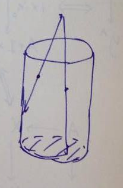
\includegraphics[scale=0.75]{retract-cofibration}
	\caption{Drawing by John Ni.}
    \end{figure}
\end{example}
In particular, $\{0,1\}\hookrightarrow I$ is a cofibration.
\section{Homotopy fibers, the Barratt-Puppe sequence}
Yesterday, I showed this:
\begin{prop}
    If $A\to X$ is a cofibration, then for any $Y$, the map $Y^X\to Y^A$ is a fibration.
\end{prop}
We did this by reverse-engineering.
\begin{example}
    $S^{n-1}\hookrightarrow D^n$ is a cofibration.
\end{example}
Let me point out properties of cofibrations.
\begin{itemize}
    \item It's closed under cobase change. What this means is if I have a cofibration $A\to X$ and any $A\to B$, then $B\to X\cup_A B$ is a cofibration.
    \item It's closed under finite products. This is surprising.
    \item It's closed under composition.
    \item Any cofibration is a closed inclusion. This is not so obvious, so check out May's book.
\end{itemize}
By the way, the dual statement would be something like: $p:E\to B$ a quotient map? No! Fibrations don't have to be surjective at all. It is surjective on path components though, because of the path-lifting stuff. But, for example, $\emptyset\to B$ is a fibration.

Another fact on fibrations is that $X\to \ast$ is a fibration, because the dotted map can be taken to the map $(t,w)\mapsto f(w)$:
\begin{equation*}
    \xymatrix{
    W\ar[d]\ar[r]^f & X\ar[d]\\
    I\times W\ar@{-->}[ur]\ar[r] & \ast
}
\end{equation*}
Model category folks get excited about this, because this says that all objects in the model structure on topological spaces is fibrant. 
\begin{definition}
Now, the inclusion $\ast\hookrightarrow X$ is not always a cofibration (see your pset!), but if it is, say that $\ast$ is a nondegenerate basepoint in $X$.
\end{definition}
Eg if $\ast$ has a neighborhood that contracts to $\ast$ then $\ast\hookrightarrow X$ is a cofibration. If $\ast$ is a nondegenerate basepoint, then $X^A\xrightarrow{ev} X$ is a fibration where $A$ is pointed. The fiber is the space of pointed maps $A\to X$.

Because $S^{n-1}\hookrightarrow D^n$ is a cofibration, we find that $\{0,1\}\hookrightarrow I$ is a cofibration. This means that the map $Y^I\to Y\times Y$ given by $\omega\mapsto (\omega(0),\omega(1))$ is a fibration. This gets into the story of path spaces.
\subsection{''Fibrant replacements''}
Don't worry about the title of this section. If you've seen model categories, this'll make sense.
\begin{theorem}
    Any map is $\simeq$ to a fibration. What does this mean? This means that for any map $f:X\to Y$ we can find a space $T(f)$ such that:
    \begin{equation*}
	\xymatrix{
	    X\ar[dr]^{\simeq}\ar[d]_f & T(f)\ar[d]^p\\
	    & Y
	    }
    \end{equation*}
    where $p$ is a fibration and $X\xrightarrow{\simeq} T(f)$ is a homotopy equivalence.
\end{theorem}
\begin{proof}
    Consider the map $Y^I\xrightarrow{\begin{pmatrix} ev_0 \\ ev_1\end{pmatrix}}Y\times Y$. Define $T(f)$ as the pullback:
	\begin{equation*}
	    \xymatrix{
		T(f)\ar[r]\ar[d] & Y^I\ar[d]^{\begin{pmatrix}ev_0 \\ ev_1\end{pmatrix}}\\
		    X\times Y\ar[r]_{f\times 1} & Y\times Y
		}
	\end{equation*}
	In other words, $T(f)=\{(x,\omega)\in X\times Y^I|f(x) = \omega(0)\}$. Let's start checking the conditions. First of all, the map $Y^I\to Y\times Y$ is a fibration. So $T(f)\to X\times Y$ is a fibration. Since $X\times Y\to Y$ is a fibration, we can consider the composite $T(f)\to X\times Y\to Y$, which is now a fibration. On elements, $T(f)\to Y$ sends $(x,\omega)\to \omega(1)$.

	To get a map $X\to T(f)$, I need to give maps $X\to X\times Y$ and $X\to Y^I$ that have compatible images in $Y\times Y$. Define $X\to X\times Y$ as $X\xrightarrow{\begin{pmatrix} 1 \\ f\end{pmatrix}}X\times Y$, and define $X\to Y^I$ as the map sending $x$ to the constant loop at $f(x)$. Clearly both composite $X\to X\times Y\\to Y\times Y$ and $X\to Y^I\to Y\times Y$ are the same, so we have a map $X\to T(f)$.

	    Is it true that the composite $X\to T(f)\xrightarrow{p} Y$ is our original map? Yes! So we only have to check that $X\to T(f)$ is a homotopy equivalence. Let me begin by constructing a homotopy inverse. I.e., a map $T(f)\to X$. We can define a map $T(f)\to X$ via $T(f)\to X\times Y\xrightarrow{pr_1} X$. Clearly the composite $X\to T(f)\to X\times Y\to X$ is the identity. This means we need to study $T(f)\to X\to T(f)$. This composite sends $(x,\omega)\mapsto x\mapsto (x,c_{f(x)})$ where $c_{f(x)}$ is the constant path at $x$. I need a homotopy between this map and the identity on $T(f)$.

	    This is what I call the spaghetti move. We know that there's no constraint on $\omega(1)$, so I can just suck it back in to get the constant loop. I guess I can define $\omega_s(t) = \omega(st)$. At $s=1$ I have $\omega$ and when $s=0$ I have $c_{f(x)} = c_{\omega(0)}$. Thus, define $I\times T(f)\to T(f)$ via $(s,(x,\omega))\mapsto (x,\omega_s)$.

	    If you want to work through the diagram, this is how it looks.
	    \begin{equation*}
		\xymatrix{
		    X\ar@{-->}[dr]\ar[drr]^{x\mapsto c_{f(x)}}\ar[ddr]_{\begin{pmatrix}1 \\ f\end{pmatrix}} & & \\
			& T(f)\ar[d]\ar[r]\ar[dr] & Y^I\ar[d]^{\begin{pmatrix}ev_0 \\ ev_1\end{pmatrix}}\\
			    X & X\times Y\ar[l]^{pr_1}\ar[d]^{pr_2}\ar[r] & Y\times Y\\
		    & Y
		    }
	    \end{equation*}
\end{proof}
Here's a really stupid example. 
\begin{example}[Path-loop fibration]
Suppose $X=\ast$. What is $T(f)$? Well it's just paths $\omega(0)$ in $Y$ such that $\omega(0)=\ast$. I.e., $T(f) = Y^I_\ast$. This is also called the path space of $Y$, denoted $P(Y,\ast)$. It's contractible by the spaghetti move. What it's fiber? The map $PY\to Y$ sends $\omega\mapsto \omega(1)$. So the fiber is the points that begin at $\ast$ and end at $\ast$. The fiber of $PY\to Y$ is denoted $\Omega Y$, which is the space of loops at $\ast$. This is called the path loop fibration. 
\end{example}
\subsection{Homotopy fibers over $\ast$}
The ordinary fiber is the pullback
\begin{equation*}
    \xymatrix{
	f^{-1}(\ast)\ar[r]\ar[d] & X\ar[d]^f\\
	\ast\ar[r] & Y
    }
\end{equation*}
\begin{definition}[Homotopy fiber]
    The homotopy fiber is the pullback:
    \begin{equation*}
	\xymatrix{
	    F(f,\ast)\ar[r]\ar[d] & T(f)\ar[r]\ar[d]^p & X\ar[dl]^f\\
	    \ast \ar[r] & Y &
	    }
    \end{equation*}
\end{definition}
As a set it's $F(f,\ast) = \{(x,\omega)\in X\times Y^I| f(x) = \omega(0), \omega(1) = \ast\}$. The ordinary fiber and the homotopy fiber are definitely not generally the same. If $W\to X\to Y$ is nullhomotopic, then it factors through $F(f,\ast)$, i.e., the composite factors as $W\to F(f,\ast)\to X\to Y$.
\begin{prop}
    Suppose $p:X\to Y$ is a fibration. Let $\ast\in Y$. Then $p^{-1}(\ast)\to F(p,\ast)$ is a homotopy equivalence.
\end{prop}
I'm not going to prove that, but you will for homework.

A different way to construct the homotopy fiber is to replace $f:X\to Y$ by a fibration. But what if I replace $\ast\to Y$ by a fibration? Namely, we now have:
\begin{equation*}
    \xymatrix{
	??\ar[r]\ar[d] & P(Y,\ast)\ar[r]^{\simeq} & \ast\ar[dl]\\
	X\ar[r] & Y & 
    }
\end{equation*}
This space $??$ consists of $(x,\omega)\in X\times Y^I$ such that $\omega(0) = \ast$ and $\omega(1) = f(x)$. Now, $F(f,\ast) = \{(x,\omega):\omega(0) = f(x), \omega(1) = \ast\}$. So $??$ is homeomorphic to $F(f,\ast)$ by reversing directions of paths. There's two ways you can produce a homotopy fiber, and all of these are homeomorphic. You could also replace both of these maps $f$ and $\ast\to Y$ by a fibration, and you'll get something that's also homeomorphic. Note that when I say $F(f,\ast)$, I'll mean $??$.

Here's what you'll prove for homework.
\begin{theorem}
    Suppose you have two fibrations $p$ and $p^\prime$ such that the following diagram commutes, where $f$ is a homotopy equivalence.
    \begin{equation*}
	\xymatrix{
	    E\ar[r]^p\ar[dr]^p & E^\prime\ar[d]^{p^\prime}\\
	    & B
	    }
    \end{equation*}
    Then $f$ is a fiber homotopy equivalence. That means that it's a homotopy equivalence in $\Top_{/B}$. What this means is that there is a map $g:E^\prime\to E$ over $B$ compatible with the fibrations and homotopies $I\times E\to E$ over $B$ and $I\times E^\prime\to E^\prime$ over $B$. I.e., the following three diagrams commute:
    \begin{equation*}
	\xymatrix{
	    E^\prime\ar[r]^g\ar[dr]^{p^\prime} & E\ar[d]^p\\
	    & B
	    }
    \end{equation*}
    and 
    \begin{equation*}
	\xymatrix{
	    I\times E\ar[r]^{1\sim gf}\ar[dr] & E\ar[d]^p\\
	    & B
	    }
    \end{equation*}
    and
    \begin{equation*}
	\xymatrix{
	    I\times E^\prime\ar[r]^{1\sim fg}\ar[dr] & E^\prime\ar[d]^{p^\prime}\\
	    & B
	    }
    \end{equation*}
\end{theorem}
So we find that for all $b$, $p^{-1}(b)\xrightarrow{\simeq} (p^\prime)^{-1}(b)$. So in particular, the fiber $F(f,\ast)$, i.e., the homotopy fiber, of $T(f)\to B$ and the fiber $f^{-1}(\ast)$ of $f:E\to B$ are homotopy equivalent if $f$ is a fibration.
\section{Barratt-Puppe sequence, $\pi_\ast$}
Hood's office hours are from 12 to 1:30 on Mondays in 2-390. Mine are from 4-5 on Tuesday in 2-478. Hood's graded the homework already.
\subsection{Fiber sequences}
Recall we have a pullback diagram:
\begin{equation*}
    \xymatrix{
	& F(f,\ast)\ar[r]\ar[d]^p & PY\ar[d]^p\ar[dr]^{\simeq} & \\
	f^{-1}(\ast)\ar[ur]\ar[r] & X\ar[r]_f & Y & \ast\ar[l]
    }
\end{equation*}
The homotopy fiber $F(f,\ast)$ thus has elements $\{(x,\sigma)\in X\times PY| f(x) = \sigma(1)\}$. We also have the ordinary fiber $f^{-1}(\ast)$. If $f$ is a fibration, the canonical map $f^{-1}(\ast)\to F(f,\ast)$ sending $x\mapsto(x,c_{f(x)})$ is a homotopy equivalence.
\begin{remark}
Consider a pointed map\footnote{Some people say ``based maps'', but it sounds like chemistry ... or evil, so I can't bring myself to say it} $f:X\to Y$, i.e., $f(\ast) = \ast$. Then I'll write $Ff$ for $F(f,\ast)$.
\end{remark}
Ok, what's the fiber of $p:Ff\to X$? The fiber over the basepoint in $X$ is precisely the space of loops in $Y$! I.e., $p^{-1}(\ast_X) = \Omega Y$, which is the space of loops in $Y$ based at $\ast_Y$. Note that this is also the homotopy fiber because $p$ is a fibration (fibrations are closed under pullbacks). So the diagram we now have is:
\begin{equation*}
\xymatrix{\\
    & \Omega Y=p^{-1}(\ast)\ar[d] & & &\\
    & F(f,\ast)\ar[r]\ar[d]^p & PY\ar[d]^p\ar[dr]^{\simeq} & \\
    f^{-1}(\ast)\ar[ur]\ar[r] & X\ar[r]_f & Y & \ast\ar[l]
}
\end{equation*}
The composite $Ff\to X\to Y$ sends $(x,\omega)\mapsto f(x)$. This is a pointed map, but not equal to the constant map. What does this even mean? Like, what is the basepoint we're choosing for $Ff$? Well, choose the basepoint to be the image of the basepoint in $f^{-1}(\ast)$ under $f^{-1}(\ast)\hookrightarrow Ff$.

We also have a (pointed!) homotopy between $Ff\to X\to Y$ and the constant map, eg via $h:Ff\times I\to Y$ defined by $h(t,(x,\omega)) = \omega(t)$. We say that the composite is \emph{nullhomotopic}. In fact, suppose $W\to X\to Y$ is nullhomotopic, with a chosen nullhomotopy -- this is the same as a map $W\to Ff$. This is a question on your homework.

Let's write $[W,X]_\ast = \pi_0(X^W_\ast)$, i.e., the pointed homotopy classes of maps $W\to X$. This is a pointed set, whose basepoint is the constant map. Ok, I can consider $[W,Ff]_\ast\to [W,X]_\ast\to [W,Y]_\ast$. This composite is nullhomotopic. But I want to say that this sequence is exact. What that means is here (because we just have pointed sets). So the preimage of the basepoint in $[W,Y]_\ast$ equals the image of $[W,Ff]_\ast\to [W,X]_\ast$. This is exactly what I said before, about nullhomotopies $W\to X\to Y$ as maps $W\to Ff$. We say that $Ff\to X\xrightarrow{f}Y$ is a \emph{fiber sequence}.

\subsection{Iterating fiber sequences}
I have $Ff\xrightarrow{p} X\xrightarrow{f} Y$. The strict fiber is $\Omega Y$, but the homotopy fiber is $Fp$. These are homotopy equivalent because $p$ is a fibration. Denote the map $i:\Omega Y\to Ff$. This sits inside:
\begin{equation*}
    \xymatrix{
	\cdots\ar[r] & Fp_3 \ar[r] & Fp_2\ar[r] & Fp_1\ar[r]^{p_2} & Ff\ar[r]^{p_1} & X\ar[r]^{f} & Y\\
	& \Omega Fp_0\ar[u]_{\simeq}\ar[ur]|{i(p_2)}\ar@{-->}[r] & \Omega X\ar@{-->}[r]\ar[u]_{\simeq}\ar[ur]|{i(p_1)} & \Omega Y\ar[u]_\simeq \ar[ur]|{i(p_0)} & &
    }
\end{equation*}
All the $p_i$s are fibrations (think about why). The dotted maps seem to be missing; I can fill them in up to homotopy, and there's one map I can think of putting there: $\Omega X\xrightarrow{\Omega f}\Omega Y$. But \emph{that's the wrong map}! The right map is $\Omega X\xrightarrow{\overline{\Omega f}}\Omega Y$ (see below for explanation). Here's a lemma.
\begin{lemma}
    The following diagram commutes to homotopy:
    \begin{equation*}
	\xymatrix{
	    & Fp\\
	    \Omega X\ar[r]_{\overline{\Omega f}}\ar[ur]^{i(p)} & \Omega Y\ar[u]
	    }
    \end{equation*}
    where $\overline{\Omega f}$ is the diagonal in:
    \begin{equation*}
	\xymatrix{
	    \Omega X\ar[r]^{-}\ar[dr]|{\Omega f} \ar[d]_{\Omega f} & \Omega X\ar[d]^{\Omega f}\\
	    \Omega Y\ar[r]_{-} & \Omega Y
	    }
    \end{equation*}
    where $-:\Omega X\to \Omega X$ sends $\omega\mapsto\overline{\omega}$.
\end{lemma}
\begin{proof}
    There is a beautiful proof of this. But it's in pictures, and I can't type it. The main point is that the proof wouldn't work unless you moved backwards. See this image:
\begin{figure}[H]
\centering
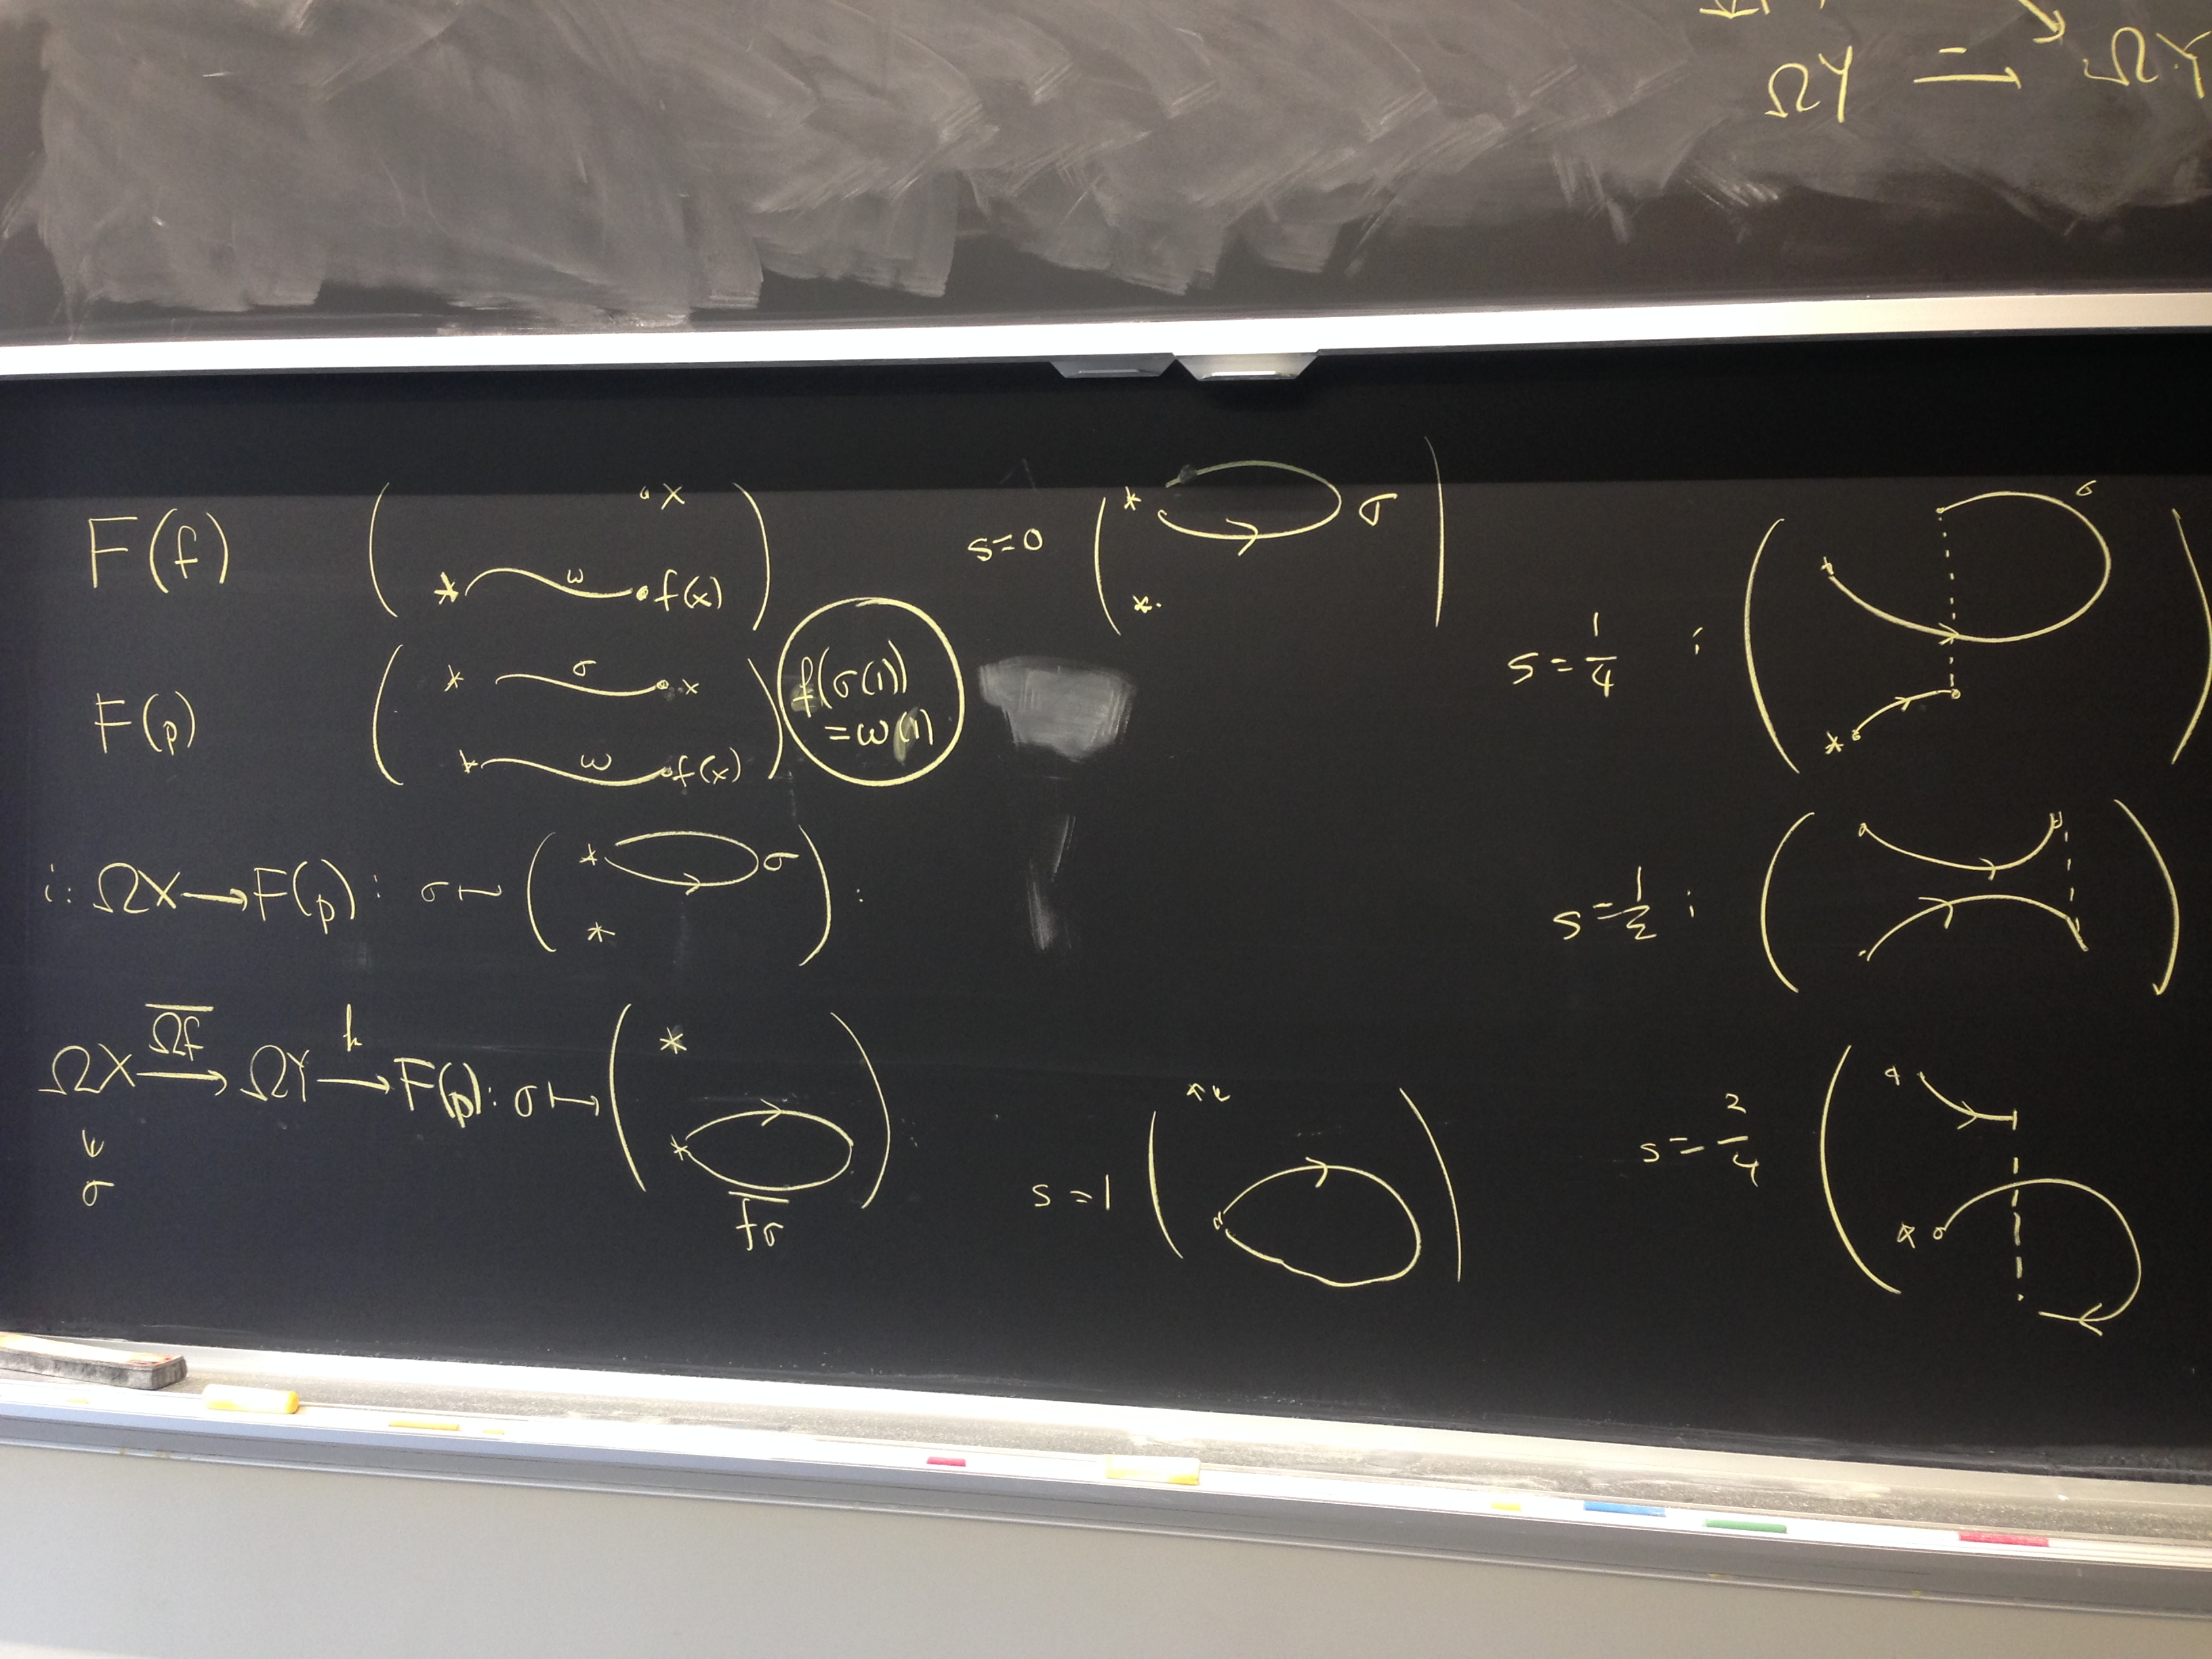
\includegraphics[width=\textwidth]{barratt-puppe}
\caption{A proof of this lemma.}
\end{figure}
\end{proof}
\begin{lemma}
    The following diagram commutes:
    \begin{equation*}
	\xymatrix{
	    & F(\overline{\Omega p_0})\ar@{=}[dd]\ar[dr] & \\
	    \Omega^2 Y\ar[ur]^{i(\Omega p_0)}\ar[dr]_{\overline{\Omega i(p_0)}} & & \Omega X\\
	    & \Omega Fp_0\ar[ur]_{\overline{\Omega p_1}} & 
	    }
    \end{equation*}
\end{lemma}
What is the map $F\overline{\Omega p_0}\to \Omega X$?? We spent some time figuring this out. But you can now apply $[W,-]_\ast$ to the following diagram to get a long exact sequence:
\begin{equation*}
    \xymatrix{
	\cdots\ar[r] & Fp_4\ar[r] & Fp_3 \ar[r] & Fp_2\ar[r] & Fp_1\ar[r]^{p_2} & Ff\ar[r]^{p_1} & X\ar[r]^{f} & Y\\
    \cdots\ar[r] & \Omega Fp_1\ar[r]|{\overline{\Omega p_2}}\ar[u]_{\simeq} & \Omega Fp_0\ar[u]_{\simeq}\ar[ur]|{i(p_2)}\ar[r]|{\overline{\Omega p}} & \Omega X\ar[r]|{\overline{\Omega f}}\ar[u]_{\simeq}\ar[ur]|{i(p_1)} & \Omega Y\ar[u]_\simeq \ar[ur]|{i(p_0)} & &\\
	\Omega^2 X\ar[u]_{\simeq}\ar[r]_{\Omega f} & \Omega Y\ar[u]_{\simeq}\ar[ur]_{\overline{\Omega i(p_0)}} & & &
    }
\end{equation*}

For example, $S^0=\{\pm 1\}$. We get terms like $\pi_0(\Omega^n X)$, because $[S^0,X] = \pi_0 X$. What is $\pi_0(\Omega^n X)$? This is $[S^0,\Omega^n X]_\ast$. Is it clear to you that this is $[S^n,X]_\ast$?

Ok, well, $\Omega^2 X = (\Omega X)^{S^1}$. Because $(S^1)^{\wedge n} = S^n$. So we find that $(\Omega X)^{S^1} = (X^{S^1}_\ast)^{S^1}_\ast = X_\ast^{S^1\wedge S^1} = X_\ast^{S^2}$.

Well, $\Omega X$ is a homotopy group by concatenation. It's a group, but where the axioms hold up to homotopy. It's a group in the homotopy category. Therefore, $\pi_0 \Omega X$ is a group! It's exactly $\pi_1 X$, which you know to be a group. And then, there's this other thing that happens.

You can think of $\pi_n(X) = [S^n,X]_\ast$ as $[(D^n,S^{n-1}),(X,\ast)] = [(I^n,\partial I^n),(X,\ast)]$. If I take $n=2$, for example, how do I take the product of $\alpha,\beta\in \pi_2(X)$? You just literally put them together (when you think of $\pi_2(X) = [(I^2,\partial I^2),(X,\ast)]$. You can play this game; up to homotopy, you can shrink $\alpha$ and $\beta$ to make them as small I want, and then reverse their position and expand them again\footnote{This probably makes no sense without a picture}\todo{Add a picture}. Thus $\pi_2(X)$ is an abelian group.

Thus, when you apply $\pi_0$ to our sequence $\cdots\to\Omega^2 X\to\Omega^2 Y\to \Omega Fp_0\to \Omega X\to \Omega Y\to Fp_0\to \Omega X\to \Omega Y$, you get an exact sequence (of groups when the homotopy groups are $>0$, and of pointed sets when you have $\pi_0$):
$$\cdots\to \pi_2 X\to \pi_2 Y\to \pi_1 Ff\to \pi_1 X\to\pi_1 Y\to\pi_0 Ff\to\pi_0 X\to \pi_0 X$$
\section{Relative homotopy, $\pi_1$ action}
Pset 2 has question 8; there's still one more to go. Hood has office hours today 12 -- 1 in 2-390, and I have office hours today tomorrow 4-5 in 2-478.
\subsection{Spheres and homotopy groups}
Let's talk about spheres, first of all. The $n$-sphere is $S^n=I^n/\partial I^n$. Agreed? It's a standard choice. By the way, $S^1 = I/0\sim 1$. What about $S^0$? This is $\ast/\emptyset = \ast_+$. This is the usual way to think of the zero sphere. The point that you just added is the basepoint.

We have this looping thing going on; we know that $\Omega X$ (I'm always working in $\Top_\ast$ these days) is $X^{S^1}_\ast$. Thus the adjunction says that $\Top_\ast(W,\Omega X) = \Top_\ast(S^1\wedge W,X)$.
\begin{definition}
    The \emph{reduced suspension} $\Sigma W$ is $S^1\wedge W$.
\end{definition}
If I have $A\subseteq X$, then $X/A\wedge Y/B = (X\times Y)/((A\times Y)\cup_{A\times B}(X\times B))$. Thus $\Sigma X = S^1\wedge X$ is $I\times X/(\partial I \times X\cup I\times \ast)$. I collapse the top and bottom of a cylinder to a point, and also the line along a basepoint gets collapsed.

Similarly, $\Sigma^n X$ is the left adjoint of the $n$-fold loop space. Hence $\Sigma^n X = (S^1)^{\wedge n}\wedge X$. What is $S^1\wedge S^n$? This is $I/\partial I\wedge I^n\wedge \partial I^n = (I\times I^n)/(\partial I\times I^n\cup I\times \partial I^n)$. This denominator is exactly $\partial I^{n+1}$; hence $S^1\wedge S^n\simeq S^{1+n}$. In fact, $S^k\wedge S^n\simeq S^{k+n}$.
\begin{definition}
    The $n$th homotopy group of $X$ is $\pi_n X = \pi_0(\Omega^n X)$.
\end{definition}
This is $[S^0,\Omega^n X]_\ast = [S^n, X]_\ast = [(I^n,\partial I^n),(X,\ast)]$.
\subsection{The homotopy category}
We have the \emph{homotopy category of spaces} $\Ho(\Top)$ whose objects are spaces and whose mapping spaces are $\pi_0$ of mapping spaces. I have to check that if $f_0,f_1:X\to Y$ and $g:Y\to Z$, then $gf_0\simeq gf_1$. Of course, it is, just by composing with $g$. Similarly $f_0h\simeq f_1h$. This guarantees that you can define composition of maps in $\Ho(\Top)$. I can also think about $\Ho(\Top_\ast)$, with pointed homotopies. A lot of what we've been doing has been taking place in $\Ho(\Top_\ast)$.

Fix $W$. We need to check that $X\mapsto X^W_\ast$ is a homotopy functor. It defines a functor $\Top_\ast\to\Top_\ast$. Namely, I want to complete:
\begin{equation*}
    \xymatrix{
	\Top_\ast\ar[d]\ar[r]^{X\mapsto X^W_\ast} & \Top_\ast\ar[d]\\
	\Ho(\Top_\ast)\ar@{-->}[r] & \Ho(\Top_\ast)
    }
\end{equation*}
So I'd better check that if I have a homotopy $f_0\sim f_1:X\to Y$. Is that a map $I\wedge X\to Y$? This really tells you that there's a nullhomotopy if the basepoint of $I$ is one of the endpoints. I really want to consider $I\times X/I\times\ast$. Aha, but this is just $I_+\wedge X$. So a homotopy $f_0\sim f_1:X\to Y$ is a map $I_+\wedge X\to Y$.

Suppose I have a homotopy like this; then I get $(I_+\wedge X)^W\to Y^W_\ast$. I wanted $I_+\wedge X^W_\ast\to Y^W_\ast$, so that's not quite what I wanted. I can get this if I can construct a map $I_+\wedge X^W_\ast\to (I_+\wedge X)^W_\ast$. In fact, I want to construct $A\wedge X^W_\ast\to (A\wedge X)^W_\ast$. One thing I can do is $A\wedge X^W_\ast\to A^W_\ast\wedge X^W_\ast$ by sending $a\mapsto c_a$, and then the exponential law gives a homotop $A^W_\ast\wedge X^W_\ast\to (A\wedge X)^W_\ast$. This gives me a map $I_+\wedge X^W_\ast\to (I_+\wedge X)^W_\ast\to Y^W_\ast$ making $X\mapsto X^W_\ast$ a homotopy functor. In particular, $\Omega^n$ is a homotopy functor.

Let's continue with this homotopical localization of things.
\begin{definition}
    A fiber sequence in $\Ho(\Top_\ast)$ is a composite $X\to Y\to Z$ that is isomorphic in $\Ho(\Top_\ast)$ to some $Ff\xrightarrow{p} E\xrightarrow{f}B$. Namely we want some (possibly zig-zag of) maps that are homotopy equivalences:
    \begin{equation*}
	\xymatrix{
	    X\ar[r]\ar[d] & Y\ar[r]\ar[d] & Z\ar[d]\\
	    Ff\ar[r]_p & E\ar[r]_f & B
	    }
    \end{equation*}
\end{definition}
We've seen examples in our elaborate story. Recall our diagram:
\begin{equation*}
    \xymatrix{
	\cdots\ar[r] & Fp_4\ar[r] & Fp_3 \ar[r] & Fp_2\ar[r] & Fp_1\ar[r]^{p_2} & Ff\ar[r]^{p_1} & X\ar[r]^{f} & Y\\
    \cdots\ar[r] & \Omega Fp_1\ar[r]|{\overline{\Omega p_2}}\ar[u]_{\simeq} & \Omega Fp_0\ar[u]_{\simeq}\ar[ur]|{i(p_2)}\ar[r]|{\overline{\Omega p}} & \Omega X\ar[r]|{\overline{\Omega f}}\ar[u]_{\simeq}\ar[ur]|{i(p_1)} & \Omega Y\ar[u]_\simeq \ar[ur]|{i(p_0)} & &\\
	\Omega^2 X\ar[u]_{\simeq}\ar[r]_{\Omega f} & \Omega Y\ar[u]_{\simeq}\ar[ur]_{\overline{\Omega i(p_0)}} & & &
    }
\end{equation*}
So look, $Ff\to X\to Y$ is a fiber sequence. And $\Omega Y\to F\xrightarrow{p}X$ is another fiber sequence because it's isomorphic to $Fp\to F\to X$ in $\Ho(\Top_\ast)$. I also have $\Omega X\xrightarrow{\overline{\Omega f}}\Omega Y\to F$ is another fiber sequence. This means that $\Omega X\xrightarrow{\Omega f}\Omega Y\to F$ is another fiber sequence because these two fiber sequences differ by an automorphism of $\Omega X$ because in general, if $A^\prime\xrightarrow{\sim} A$ and $A\to B\to C$ is a fiber sequence, so is $A^\prime\xrightarrow{\sim} A\to B\to C$.

I can apply $\Omega$ again, so I get $\Omega F\xrightarrow{\Omega p} \Omega X\xrightarrow{\Omega f} \Omega Y$. I claim this is a fiber sequence, because this is a loop of a fiber sequence, and taking loops takes fiber sequences to fiber sequences. This is called the \emph{Barratt-Puppe sequence}. I carefully explained that this makes some sense, because it firstly makes sense to ask that $\Omega$ is a homotopy functor. I haven't said this yet. So in particular:
\begin{enumerate}
    \item $\Omega$ takes fiber sequences to fiber sequences.
    \item $\Omega Ff\simeq F\Omega f$. Check this!
\end{enumerate}
You can now \emph{loop back} to get $\Omega^2 Y\xrightarrow{\Omega i} \Omega F\xrightarrow{\Omega p}\Omega X$. This is an unstable version of a triangulated category. It wants to be a triangulated category, but it isn't.
\begin{remark}
    If $f:X\to Y$, I can form $Ff$. I might have a homotopy commuting diagram like:
    \begin{equation*}
	\xymatrix{
	    \Omega Y\ar[d]_{\Omega g}\ar[r] & Ff\ar@{-->}[d]\ar[r] & X\ar[d]_{h}\ar[r]^f & Y\ar[d]^g\\
	    \Omega Y^\prime\ar[r] & Ff^\prime\ar[r] & X^\prime\ar[r]_{f^\prime} & Y
	    }
    \end{equation*}
    The dotted map exists, but \emph{this map depends on the homotopy} $f^\prime h\simeq gf$. That's an important subtlety.
\end{remark}
\subsection{Lexseq of a fiber sequence}
Applying $\pi_0 = [S^0,-]_\ast$ to the Barratt-Puppe sequence gives a lexseq:
\begin{equation*}
    \xymatrix{
	& \cdots\ar[r] & \pi_2 Y\ar[dll]\\
	\pi_1 F\ar[r] & \pi_1 X\ar[r] & \pi_1 Y\ar[dll]\\
	\pi_0 F\ar[r] & \pi_0 X\ar[r] & \pi_1 X
    }
\end{equation*}
of pointed sets. But this is even better, ,because $\Omega X$ is a group object in $\Ho(\Top_\ast)$.
\begin{remark}
    $\Ho(\Top)$ and $\Ho(\Top_\ast)$ has products and coproducts, but very few other limits or colimits. So as a category, it is \emph{horrible}.
\end{remark}
I showed you an argument that $\Omega^2 X$ is an \emph{abelian} group object, i.e., multiplication is commutative up to homotopy. Thus $\pi_1$ is a group and $\pi_k$ is an abelian group for $k\geq 2$; hence in our diagram above, all maps (except on $\pi_0$) are group homomorphisms!

What if $X\to Y$ is the inclusion $i:A\hookrightarrow X$ of a subspace? Then $Fi=\{(a,\omega)\in A\times X^I_\ast|\omega(1) = a\}$. This is just the collection of all paths that begin at $\ast\in A$ and ends in $A$.
\begin{definition}
    $\pi_n(X,A,\ast) = \pi_n(X,A)$ is $\pi_{n-1}Fi = [(I^n,\partial I^n,(\partial I^n\times I)\cup (I^{n-1}\times 0)),(X,A,\ast)]$.
\end{definition}
Inside $I^n$ is $\partial I^n$, and also including in it is $\partial I^n\times I\cup I^{n-1}\times 0$. Then you can check that $\pi_{n-1}Fi = [(I^n,\partial I^n,(\partial I^n\times I)\cup (I^{n-1}\times 0)),(X,A,\ast)]$. In this case, you have a lexseq: 
\begin{equation*}
    \xymatrix{
	& \cdots\ar[r] & \pi_2 (X,a)\ar[dll]\\
	\pi_1 A\ar[r] & \pi_1 X\ar[r] & \pi_1 (X,A)\ar[dll]\\
	\pi_0 A\ar[r] & \pi_0 X\ar[r] & 
    }
\end{equation*}
\section{Action of $\pi_1$, simple spaces, and the Hurewicz theorem}
Recall that $\pi_n(X,A,\ast) = [(I^n,\partial I^n,\partial I^{n-1}\times I\cup I^{n-1}\times 0),(X,A,\ast)]$. You have a lexseq of the form:
\begin{equation*}
    \xymatrix{
	& \cdots\ar[r] & \pi_2 (X,a)\ar[dll]\\
	\pi_1 A\ar[r] & \pi_1 X\ar[r] & \pi_1 (X,A)\ar[dll]\\
	\pi_0 A\ar[r] & \pi_0 X\ar[r] & 
    }
\end{equation*}
This looks very similar to the lexseq for homology. How does this actually relate?
\begin{lemma}[Excision]
    If $A\subseteq X$ is a cofibration, then there is an isomorphism $H_\ast(X,A)\xrightarrow{\simeq}\widetilde{H}_\ast(X/A)$. Under this hypothesis, $X/A\simeq\text{Mapping cone of }i:A\to X$. The mapping cone is the dual to the homotopy fiber, i.e., the homotopy quotient, which is defined by the pushout:
    \begin{equation*}
	\xymatrix{
	    A\ar[r]^i\ar[d]^{in_1} & X\ar[d]\\
	    CA\ar[r] & X\cup_A CA
	    }
    \end{equation*}
    where $CA$ is the cone on $A$ defined as $CA = A\times I/A\times 0$ (this is a contractible space).
\end{lemma}
This is dual to saying that $Ff\simeq f^{-1}(\ast)$ if $f$ is a fibration.

But $\pi_\ast(X,A)$ is definitely not $\pi_\ast(X/A)$! For example, $S^1\to D^2\to S^2$ is a cofibration sequence, but $\pi_\ast S^1$ is just $\Z$ in dimension $1$. We don't know the homotopy groups of $S^2$, though. In fact:
\begin{theorem}[Now]
    If $X$ is a simply connected finite complex, and $X\not\simeq \ast$, then we do not know $\pi_\ast(X)$. And we'll probably never be able to know them.
\end{theorem}
These groups \emph{are} computable (a theorem by Edgar Brown), but it's super-exponential. This is discouraging. We'll never know what, eg., $\pi_{10000}(S^2)$ is.

Anyway, I said there was $\partial:\pi_n(X,A,\ast)\to \pi_{n-1}(A,\ast)$. How does this look? Well you just look at the restriction of $I^n\to X$ to $1\times I^{n-1}\to A$. And the composite $\pi_n(X,A,\ast)\xrightarrow{\partial}\pi_{n-1}(A,\ast)\to \pi_{n-1}(X,\ast)$ is trivial by definition!
\subsection{$\pi_1$-action}
There's a little more structure about this sequence. That's the following thing: $\pi_1(X)$ acts on $\pi_n(X)$ from the left by group homomorphisms. There was a picture, but I didn't understand it. Let me write this out (as I understand it). Suppose $x,y\in X$, and let $\omega:I\to X$ with $\omega(0) = x$ and $\omega(1) = y$. Then we have a map $f_\omega:\pi_n(X,x)\to \pi_n(X,y)$, so $\pi_1(X,\ast)$ acts on $\pi_n(X,\ast)$.

When $n=1$, $\pi_1(X)$ acts by conjugation. In fact, $\pi_1(A)$ acts on $\pi_n(X,A,\ast)$ as well. It then follows that all maps in the lexseq are equivariant for this action of $\pi_1(A)$. We also have the Peiffer identity:
\begin{prop}[Peiffer identity]
    let $\alpha,\beta\in \pi_2(X,A)$. Then $(\partial \alpha)\cdot\beta = \alpha\beta\alpha^{-1}$.
\end{prop}
For example, if $j:\pi_2(X)\to \pi_2(X,A)$, and $\alpha = j(\gamma)$, $\partial\alpha = 1$: $\img(k)\subseteq\coker \pi_2(X,A)$. (I did not follow this)

\begin{definition}
    $X$ is simply connected if it's path connected and $\pi_1(X,\ast) = 1$.
\end{definition}
Sometimes you have nontrivial $\pi_1$, and so:
\begin{definition}
    $X$ is \emph{simple} if it is path-connected and $\pi_1(X)$ acts trivially on $\pi_n(X)$ for $n\geq 1$.
\end{definition}
(In particular, $\pi_1(X)$ is abelian.) What does being simple do for you?
\begin{itemize}
    \item Being simple is independent of the choice of basepoint. If $\omega:x\to x^\prime$, then $\omega_\sharp:\pi_n(X,x)\to \pi_n(X,x^\prime)$ is a group isomorphism. I have $\pi_1(X,x)$ acting on $\pi_n(X,x)$ and $\pi_1(X,x^\prime)$ acting on $\pi_n(X,x^\prime)$. These actions are compatible, and if $\pi_1(X,x)$ acts trivially then so does $\pi_1(X,x^\prime)$.
    \item Say $X$ is path-connected. Then there's a map $\pi_n(X,\ast)\to [S^n,X]$. It's pretty obvious that this map is surjective because I can always choose a basepoint in $X$ as the image of a basepoint in $S^n$. Thus you'd expect a factorization:
	\begin{equation*}
	    \xymatrix{
		\pi_n(X,\ast)\ar@{->>}[r]\ar[dr] & [S^n,X]\\
		& \pi_1(X,\ast)\backslash \pi_n(X,\ast)\ar[u]_{\cong,\text{homework}}
		}
	\end{equation*}
	If $X$ is simple, then $\pi_1(X,\ast)\backslash \pi_n(X,\ast)$ is trivial, and so $\pi_n(X,\ast)\cong [S^n,X]$ that's independent of the basepoint. I.e., these groups are canonically the same, i.e., two paths $\omega,\omega^\prime:x\to y$ give the same map $\omega_\sharp = \omega^\prime_\sharp:\pi_n(X,x)\to \pi_n(X,y)$.
\end{itemize}
\subsection{Hurewicz theorem}
I talked about homotopy, and I talked about homology. Now it's time to compare the two. This is the story of the Hurewicz theorem. You should think of homology of being computable, while homotopy is a big mystery.
\begin{definition}
The Hurewicz map is a map $h:\pi_n(X,\ast)\to H_n(X)$, where $X$ is a path connected space. How does this map go? An element in $\pi_n(X,\ast)$ is represented by $\alpha:S^n\to X$. Pick a generator $\sigma:H_n(S^n)$; then $\alpha_\ast(\sigma)\in H_n(X)$.
\end{definition}
This is a homomorphism, as I'll show in a bit.

What happens when $n=0$? What map $\pi_0(X)\to H_0(X)$ do we have? A point is like a $0$-cycle, and that's the map! In fact, we have an isomorphism $H_0(X)\simeq \Z[\pi_0(X)]$. This is an example of the Hurewicz theorem.

How about $n=1$? Now, we have $h:\pi_1(X,\ast)\to H_1(X)$. This factors as $\pi_1(X,\ast)\to \pi_1(X,\ast)^{ab}\to H_1(X)$. And the Hurewicz theorem says that $\pi_1(X,\ast)^{ab}\xrightarrow{\simeq} H_1(X)$. I'm not going to prove this; it's not very hard but it's annoying. It's pretty clear why it's true: for example, it's onto. $1$-cycles just look like a bunch of circles, so just concatenate loops from the basepoint to these $1$-cycles.

Let me show you that the Hurewicz map is a homomorphism. Before that, here's the Hurewicz theorem.
\begin{theorem}[Hurewicz]
    Suppose $\pi_i(X) = 0$ for $i<n$ where $n\geq 2$. Then $\pi_n(X)\xrightarrow{\simeq}H_n(X)$.
\end{theorem}
We can't compute homotopy in general, but we can at least make a start.

OK, why is $h$ a homomorphism? Let $\alpha,\beta:S^n\to X$ be pointed maps. What is the product in $\pi_n(X)$? It's just the composite:
$$\alpha\beta:S^n\xrightarrow{\delta\text{, pinching along the equator}} S^n\vee S^n\xrightarrow{\beta\vee\alpha}X\vee X\xrightarrow{\nabla\text{, the fold map}}X$$
where $\nabla:X\vee X\to X$ is defined by:
\begin{equation*}
    \xymatrix{
	X\ar[dr]^1\ar[d] & \\
	X\vee X\ar[r]|\nabla & X\\
	X\ar[u]\ar[ur]_1 & 
    }
\end{equation*}
We have two inclusions $in_1,in_2$ of $S^n$ to $S^n\vee S^n$. Now, we have:
$$\sigma\mapsto {in_1}_\ast\sigma + {in_2}_\ast\sigma\mapsto {in_1}_\ast h(\alpha) + {in_2}_\ast h(\beta)\mapsto h(\alpha) + h(\beta)$$
As desired. It's possible to give an elementary proof of Hurewicz's theorem. But I'll prove this as a consequence of the Serre spectral sequence, which gives a more genral theorem. It'll be an inductive proof that'll use Poincare's result.

One more thing to say is that $\pi_i(S^n) = 0$ if $i<n$. I won't prove this, but it's also kind of obvious, isn't it? By Hurewicz, it follows that $\pi_n(S^n)\simeq H_n(S^n)\simeq \Z$. We actually have one more example: $\pi_3(S^2)\simeq \Z$ generated by the Hopf fibration $S^3\to S^2$. It's not obvious that this isn't nullhomotopic, but it's true. But now, for example, I can suspend $\eta$ (the Hopf fibration) and get $\eta\circ\Sigma\eta$. We thought for a long time that there were the only things we could compute in $\pi_\ast S^n$; but this is not true! It's a lot more chaotic.
\section{Some examples; CW complexes}
\subsection{Examples}
\begin{enumerate}
    \item Let $E\to B$ be a covering space with $E$ and $B$ connected. The fibers are discrete, so they don't have any higher homotopy. There's only $\pi_0$. The lexseq says that $\pi_n(E)\to \pi_n(B)$ is an isomorphism for $n>1$, and $\pi_1(E)\hookrightarrow \pi_1(B)$, and the subgroup $\pi_1(E)$ classifies the covering space. In general, we know that $\Omega B$ acts on the homotopy fiber $F$. Because $F$ here is discrete, this action factors through $\pi_0(\Omega B)\simeq \pi_1(B)$.

	In particular, $\pi_q(S^n)\simeq \pi_q(\RP^n)$ for $q>1$. Of course, $\pi_1(\RP^n)\simeq \Z/2\Z$. This creates a ton of homology in $\RP^n$ that's not present in the homology of $S^n$. Here's a piece of language.

	\begin{definition}
	    A space is \emph{$n$-connected} if $\pi_i(X) = 0$ for $i\leq n$.
	\end{definition}
	This is not a nonsense definition, although it seems like we need to pick a basepoint -- but $0$-connected means path connected, so we're good. For instance, $1$-connected means simply connected.

	Suppose $E\to B$ is a covering space where $E$ is $n$-connected. Then $\pi_1(B)$ determines the homology $H_i(B)$ in dimensions $i<n$. In particular, $H_i(B) = H_i(\pi_1(B))$, which is the group homology. This is due to Heinz Hopf.
    \item What's a nontrivial action of $\pi_1$ on higher homotopy? For example, $\pi_1$ acting on $\pi_2$. Consider the space $S^1\vee S^2$. What does the universal cover $E$ look like? This just $\RR$, where at every integer point I put a $2$-sphere $S^2$. The universal cover is simply connected, so Hurewicz says that $\pi_2(E)\simeq H_2(E)$. Up to homotopy type, I can collapse the line to a point, so I get a countable bouquet of $2$-spheres. Thus $\pi_2(E)\simeq H_2(E) = \bigoplus^\infty\Z$. But I can say more!

	There's an action of $\pi_1(S^1\vee S^2)$ on $E$. Certainly $\pi_1(S^1\vee S^2) = \Z$. There's an induced action on $E$. All the action does is shift the $2$-spheres on the integer points of $\RR$ (on $E$) to the right by $1$. Thus $\bigoplus^\infty\Z=\Z[\pi_1(B)]$ as a $\Z[\pi_1(B)]$-module (i.e., as a $\Z[\Z]$-module). That's actually the same action of $\pi_1(E)$ on $\pi_2(E)$.	This tells something horrifying. $S^1\vee S^2$ is a very simple $3$-complex, but its homotopy is huge.
    \item $\pi_\ast(X)=?$. Recall our Hopf fibration $S^1\to S^3\to S^2$. This gives a lexseq on homotopy groups. Thus I get $\pi_i(S^3)\xrightarrow{\simeq}\pi_i(S^2)$ for $i>2$ given by $\alpha\mapsto\eta\alpha$. Of course, $\pi_2(S^2) = \Z$. The higher homotopy groups of $S^2$ are exactly the same as the higher homotopy groups of $S^3$! In particular, $\pi_3(S^3)=\Z$ by Hurewicz, so $\pi_3(S^2)\simeq \Z$ generated by $\eta$. There are some low-dimensional calculations that you can make like this.

	Here's another way of thinking of the Hopf fibration. Think of $S^3 = SU(2)$. Then there's the subgroup of $\begin{pmatrix}\lambda & \\ & \lambda^{-1}\end{pmatrix}$, which is $S^1$. This acts on $S^3$ by translation, and the orbit space is $S^2$.

	We'll show later that $\pi_{4n-1}(S^{2n})\otimes\QQ\simeq \QQ$. Other than $\pi_n(S^n)$, a theorem of Serre says that these are the only non-torsion homotopy groups of spheres.
\end{enumerate}
\subsection{Bringing you up-to-speed on CW-complexes}
I want to study a fairly rich example of CW-complexes.
\begin{definition}
    A \emph{relative} CW-complex is a pair $(X,A)$ together with a fitration $A=X_{-1}\subseteq X_0\subseteq X_1\subseteq\cdots\subseteq X$, such that for all $n$, I can build $X_n$ as the pushout:
    $$
    \xymatrix{
	\coprod_{\alpha\in \Sigma_n}S^{n-1}\ar[r]\ar[d]_{\text{attaching maps}} & \coprod_{\alpha\in \Sigma_n}D^n\ar[d]^{\text{characteristic maps}}\\
	X_{n-1}\ar[r] & X_n
    }
    $$
    ($X_n$ is called the $n$-skeleton), and $X=\varinjlim X_n$.
\end{definition}
If $A=\emptyset$, it's not relative anymore -- it's just a CW-complex. (Here $S^{-1} = \emptyset$.) Often, $X$ will be a CW-complex, and $A$ will be a subcomplex.
\begin{enumerate}
    \item If $A$ is Hausdorff, then so is $X$. Actually, last semester I discovered a proof of this in Hatcher.
    \item $A=\emptyset$: then $X$ is compactly generated. This is one of the reasons I wanted to define compactly generated spaces.
    \item If $X$ and $Y$ are both CW-complexes. Then define $(X\times^k Y)_n = \bigcup_{i+j = n}X_i\times Y_j$. This gives a CW-structure on the product $X\times^k Y$.
    \item Any closed smooth manifold admits a CW-structure. 
\end{enumerate}
The fun example is $\CP^n$.
\begin{example}
    $\CP^n$ is a CW-complex, with skeleta $\CP^0\subseteq\CP^1\subseteq\cdots\subseteq \CP^n$. The assertion is that there's a pushout diagram:
    \begin{equation*}
	\xymatrix{
	    \coprod S^{2n-1}\ar[r]\ar[d] & \coprod D^{2n}\ar[d]\\
	    \CP^{n-1}\ar[r] & \CP^n
	    }
    \end{equation*}
    Any complex line through the origin meets the hemisphere defined by $\begin{pmatrix}z_0\\\vdots\\z_n\end{pmatrix}$ with $||z||=1$ and $\Im(z_n) = 0$ and $\Re(z_n)\geq 0$. It meets this hemisphere (which is $D^{2n}$) at one point, unless it's on the equator, in which case we find that the pushout diagram is really:
    \begin{equation*}
	\xymatrix{
	    S^{2n-1}\ar[r]\ar[d] & D^{2n}\ar[d]\\
	    \CP^{n-1}\ar[r] & \CP^n
	    }
    \end{equation*}
\end{example}
I want to give you a more complicated example that's fun and that will come up later.
\begin{example}[Grassmannians]
    Let $V=\RR^n$ or $\cc^n$ or $\HH^n$. Let's suppose $V=\RR^n$ for now. Then $\Gra_k(\RR^n)$ is the collection of $k$-dimensional subspaces of $\RR^n$. One way to do this is by giving a $k\times n$ rank $k$ matrix. Here's some linear algebra.

    The span of rows of $A$ is the row space $V_A$. This is the span of the rows of the reduced reduced echelon form of $A$. An entry is a \emph{pivot} if its leftmost nonzero is in its row. A column is \emph{pivotal} if it contains a pivot. Any matrix is reduced echelon if the $i$th pivotal column is $e_i$.

    For instance, $\Gra_2(\RR^4)$ is as a set the disjoint union of:
    \begin{equation*}
	\begin{pmatrix}& 1 & \\ & & 1\end{pmatrix},\begin{pmatrix}&1&\ast\\&&1\end{pmatrix},\begin{pmatrix}1&\ast&\ast\\&&1\end{pmatrix},\begin{pmatrix}&1&\ast\\&1&\ast\end{pmatrix},\begin{pmatrix}1&\ast&\ast\\&1&\ast\end{pmatrix},\begin{pmatrix}1&\ast&\ast\\1&\ast&\ast\end{pmatrix}
    \end{equation*}
    So, define:
    \begin{definition}
	$\mathrm{sk}_j\Gra_k(\RR^n)$ is $\{V:\text{row ech rep with $\leq j$ free entries}\}$.
    \end{definition}
    The claim is that it's a CW-structure. See Milnor-Stasheff. They don't know it in 18.06, but they're constructing a CW-structure for the Grassmannian.
\end{example}
    The complex Grassmannian has cells in only even dimensions. We now know what the homology of the Grassmannian is, so we actually find Poincare duality if we count the number of cells in this case. (This is visible, for instance, in $\Gra_2(\RR^4)$). By the way, the top-dimensional cell tells us that $\dim\Gra_k(\RR^n) = k(n-k)$.
\section{Relative Hurewicz and J.~H.~C.~Whitehead}
I find what I'm talking about today very confusing, because there's this number, this $n$. I'm going to essentially read from my notes, because I'll get confused otherwise.
\begin{definition}
    Let $n\geq 0$. Say that $X$ is $(n-1)$-connected if for all $0\leq k\leq n$, and any $f:S^{k-1}\to X$ extends:
    \begin{equation*}
	\xymatrix{
	S^{k-1}\ar[d]\ar[r] & X\\
	D^k\ar@{-->}[ur] & 
	}
    \end{equation*}
\end{definition}
    Let's see what happens in low dimensions. When $n=0$, we know that $S^{-1} = \emptyset$, and $D^0 = \ast$. Saying that you're $(-1)$-connected is just saying that you're nonempty. If $n=1$, then this is saying that you're path connected, i.e., $0$-connected iff path connected. You can check that this is exactly the same as what we said before, using homotopy groups.

\begin{definition}
    Let $n\geq 0$. Say that $(X,A)$ is $n$-connected if for all $0\leq k\leq n$, there's a lift:
    \begin{equation*}
	\xymatrix{
	    (D^k,S^{k-1})\ar[r]^f\ar@{-->}[d] & (X,A)\\
	    (A,A)\ar[ur] & 
	    }
    \end{equation*}
    up to homotopy. In other words, you can homotope $f$ to a map with image in $A$, without moving $f|_{S^{k-1}}$.
\end{definition}
What does this mean for small values? When $n=0$, we find that $0$-connected means that $A$ meets every path component of $X$.

Equivalently, we can state:
    \begin{definition}
	$(X,A)$ is $n$-connected if:
	\begin{itemize}
	    \item $n=0$: then $\pi_0(A)\to \pi_0(X)$ surjects.
	    \item $n>0$: then $\pi_0(A)\xrightarrow{\simeq}\pi_0(X)$, and for all $a\in A$, $\pi_k(X,A,a) = 0$ for $1\leq k\leq n$. Equivalently, $\pi_0(A)\xrightarrow{\simeq}\pi_0(X)$ and $\pi_k(A,a)\to\pi_k(X,A)$ is an isomorphism for $1\leq k<n$ and is onto for $k=n$.
	\end{itemize}
    \end{definition}
    So ``$\pi_0(X,A) = 0$'' makes sense, because it means $\pi_0(A)\to \pi_0(X)$ surjects. I can't define $\pi_0(X,A)$, but you should think of it this way.

Let's try to write down what the relative Hurewicz theorem might be.
\subsection{Relative Hurewicz}
    Assume that $\pi_0(A) = \ast = \pi_0(X)$, and pick $a\in A$, which I won't bother about any more. We have:
    \begin{equation*}
	\xymatrix{
	    \cdots\ar[r] & \pi_2(X,A)\ar[r]\ar[d]^h & \pi_1(A)\ar[r]\ar[d]^h & \pi_1(X)\ar[r]\ar[d]^h & \pi_1(X,A)\ar[r]\ar[d]^h & \pi_0(A)\ar[r]\ar[d]^h & \pi_0(X)\ar[d]^h & \\
	    \cdots\ar[r] & H_2(X,A)\ar[r] & H_1(A)\ar[r] & H_1(X)\ar[r] & H_1(X,A)\ar[r] & H_0(A)\ar[r] & H_0(X)\ar[r] & H_0(X,A)
	    }
    \end{equation*}
How do we define the relative Hurewicz map? Let $\alpha\in \pi_n(X,A)$; then $\alpha:(D^n,S^{n-1})\to (X,A)$. So we pick a generator in $\Z\in H_n(D^n,S^{n-1})$, and send it to something in $H_n(X,A)$ under the induced $\alpha^\ast:H_n(D^n,S^{n-1})\to H_n(X,A)$.

Because $H_n(X,A)$ is abelian, we find that $\pi_1(A)$ acts trivially on $H_n(X,A)$, i.e., $h(\omega(\alpha)) = h(\alpha)$. Thus the relative Hurewicz map factors through $\pi_n^\dagger(X,A)$, which is $\pi_n(X,A)$ quotiented out by the normal subgroup generated by $(\omega\alpha)\alpha^{-1}$ where $\omega\in\pi_1(A)$ and $\alpha\in \pi_n(X,A)$. Thus you get a map $\pi_n^\dagger(X,A)\to H_n(X,A)$, that's more likely to be an isomorphism.
\begin{theorem}[Relative Hurewicz]
    Let $n\geq 1$. Assume $(X,A)$ is $n$-connected. Then $H_k(X,A) = 0$ for $0\leq k\leq n$, and $\pi_{n+1}^\dagger(X,A)\to H_{n+1}(X,A)$ is an isomorphism.
\end{theorem}
\begin{proof}
I won't prove this now; with any luck, we'll come back and prove this once we have the Serre spectral sequence in our toolkit.
\end{proof}
This is an extremely useful result. Now, that's it! That's all I wanted to say about the relative Hurewicz theorem. Let's apply this to get surprising results.
\subsection{J.~H.~C.~Whitehead theorems}
He was an interesting character. He raised pigs. He's interested in a continuous map $f:X\to Y$, and when that's an isomorphism in homology or homotopy, and relate them.
\begin{definition}
    Let $f:X\to Y$ and $n\geq 0$. Say that $f$ is an $n$-equivalence (some would say $n$-connected, but I won't say that here) if for every $\ast\in Y$, the homotopy fiber $F(f,\ast)$ is $(n-1)$-connected.
\end{definition}
A $0$-equivalence means that $\pi_0(X)$ surjects onto $\pi_0(Y)$. For $n>0$, this is saying that $\pi_0(X)\xrightarrow{\simeq}\pi_0(Y)$, and for every $\ast\in X$:
\begin{equation*}
    \pi_k(X,\ast)\to\pi_k(Y,f(\ast)) \text{ is }\begin{cases}
	\text{iso } & 1\leq k<n\\
	\text{epi, i.e., onto } & k = n
    \end{cases}
\end{equation*}
Would you like me to tell you about how to replace a map by a cofibration? Never mind -- this is the first problem! So, using the ``mapping cylinder'', we can always assume $f:X\hookrightarrow Y$, and then $f:X\to Y$ is an $n$-equivalence iff $(Y,X)$ is $n$-connected.
\begin{theorem}[J.~H.~C.~Whitehead 1]
    Suppose $n\geq 0$, and $f:X\to Y$ is $n$-connected. Then:
\begin{equation*}
H_k(X)\to H_k(Y) \text{ is }\begin{cases}
\text{iso } & 1\leq k<n\\
\text{epi, i.e., onto } & k = n
\end{cases}
\end{equation*}
\end{theorem}
\begin{proof}
    When $n=0$, because $\pi_0(X)\to \pi_0(Y)$ is surjective, $H_0(X)\simeq \Z[\pi_0(X)]\to \Z[\pi_0(Y)]\simeq H_0(Y)$ is surjective. The relative Hurewicz theorem gives the rest. Note that the relative Hurewicz dealt with $\pi_n^\dagger(X,A)$, but $\pi_n(X,A)\to\pi_n^\dagger(X,A)$ is surjective.
\end{proof}
Let me call out what happens when $n=\infty$.
\begin{definition}
    $f$ is a \emph{weak equivalence} (or an $\infty$-equivalence, to make it sound more impressive) if it's an $n$-equivalence for all $n$, i.e., it's a $\pi_\ast$-isomorphism.
\end{definition}
Putting everything together, we obtain:
\begin{corollary}
    A weak equivalence induces an isomorphism in integral homology.
\end{corollary}
Let's try to go in the other direction.

If $H_0(X)\to H_0(Y)$ surjects, then $\pi_0(X)\to \pi_0(Y)$ surjects also. Good start! Assume $X$ and $Y$ path connected. Suppose $H_1(X)$ surjects onto $H_1(Y)$. I'd like to know that $\pi_1(X)\to\pi_1(Y)$ surjects. It's hard to know this, though, because $H_1(X)$ is the abelianization. Let's give up and assume that $\pi_1(X)\to \pi_1(Y)$ is surjective.

Assume $\pi_1(X)$ surjects onto $\pi_1(Y)$. Assume $H_2(X)\to H_2(Y)$ surjects, and $H_1(X)\xrightarrow{\simeq}H_1(Y)$ surjects. We know that $H_2(Y,X) = 0$. On the level of the Hurewicz maps, I still don't know what to do because I only know about $\pi_2^\dagger$. What to do? Let's assume that $\pi_1(X)$ is trivial. That's a pretty radical assumption. It'd be enough to ask that $\pi_1(X)$ acts trivially on $\pi_2(Y,X)$. That's \emph{technically} what you want to assume. That's basically impossible to check. Anyway, if $\pi_1(X) = 0$, then $\pi_1(Y) = 0$. So $\pi_2(Y,X)$ is trivial, and we can go up the ladder.
\begin{theorem}[J.~H.~C.~Whitehead 2]
    Let $n\geq 2$. Assume that $\pi_1(X) = 0 = \pi_1(Y)$, and I have $f:X\to Y$ such that:
\begin{equation*}
H_k(X)\to H_k(Y) \text{ is }\begin{cases}
\text{iso } & 1\leq k<n\\
\text{epi, i.e., onto } & k = n
\end{cases}
\end{equation*}
then $f$ is an $n$-equivalence.
\end{theorem}
\begin{corollary}
    Let $X$ and $Y$ be simply-connected. If $f$ induces an isomorphism in homology, then it's a weak equivalence.
\end{corollary}
That's an \emph{incredibly} useful theorem, because we can actually compute homology! Let's complete this with a further theorem we'll prove on Wednesday.
\begin{theorem}
    If $Y$ is a CW-complex, a weak equivalence $f:X\to Y$ is in fact a homotopy equivalence!
\end{theorem}
\section{Cellular approximation, cellular homology, obstruction theory}
pset 3 is up in part. Today I'm going to tell you how to think about CW-complexes and work with them, and I won't give a lot of details. Some good sources are lecture notes by Davis-Kirk, and a beautiful book by Glen Bredon, as well as Hatcher.
\subsection{Cellular approximation}
\begin{theorem}
    Let $X$ and $Y$ be CW-complexes and $A\subseteq X$ a subcomplex. Let $f:X\to Y$ be a continuous map, and that $f|_{A}$ is skeletal\footnote{Some people would say cellular.}, i.e., $f(\Sigma_n)\subseteq Y_n$. It might not take cells in $A$ to cells in $Y$, but it takes $n$-skeleta to $n$-skeleta. Then $f$ is homotopic to some other $f^\prime:X\to Y$ relative to $A$ with $f^\prime$ skeletal on all of $X$.
\end{theorem}
This is kind of amazing.
\begin{lemma}[Key lemma]
    Any $(D^n,S^{n-1})\to (Y,Y_{n-1})$ compresses through:
    \begin{equation*}
	\xymatrix{
	(D^n,S^{n-1})\ar[r]\ar@{-->}[dr] & (Y,Y_{n-1})\\
	& (Y_n,Y_{n-1})\ar[u]
	}
    \end{equation*}
\end{lemma}
\begin{proof}[``Proof.'']
    I take this as obvious, but here's something. Since $D^n$ is compact, we know that $f(D^n)$ must lie in some finite subcomplex $K$ of $Y$. Now the map $D^n\to K$ might hit some top-dimensional cell $e^m\subseteq K$, which doesn't have anything attached to it, so I can poke a hole in it (namely the approximate this so that you miss a point) and it contracts onto a lower-dimensional cell. Iterating this process gives the desired result.
\end{proof}
Let's see why the theorem is true based on this lemma.
\begin{proof}[``Proof'' of the cellular approximation theorem]
    I'm going to make this homotopy $f\simeq f^\prime$ one cell at a time. I might as well replace $A$ by whatever I've extended the homotopy to. So I have a single cell attachment $A\to A\cup D^m$. We have:
    \begin{equation*}
	\xymatrix{
	A\ar[d]_{\text{skeletal}}\ar[r] & A\cup D^m\ar[dl]^{\text{may not be skeletal}}\\
	Y &
	}
    \end{equation*}
    Now we're to use the compression lemma to get $A\cup D^m\to Y_m$. I'm not satisfied, because I have to do something about the rest of $X$. Here's a wonderful fact: the inclusion of a subcomplex is a cofibration. Thus we can extend this to a map from $X$, and iterate to get what we want.

    Why's the wonderful fact true? We have a cofibration $S^{n-1}\to D^n$, so any coproduct of these is a cofibration, and the pushout of a cofibration is a cofibration.
\end{proof}
\begin{corollary}[Homework]
    The pair $(X,X_n)$ is $n$-connected.
\end{corollary}
\subsection{Cellular homology}
Let $(X,A)$ be a relative CW-complex with $A\subseteq X_{n-1}\subseteq X_n\subseteq\cdots\subseteq X$. We showed last fall that $H_\ast(X_n,X_{n-1})\simeq \widetilde{H}_\ast(X_n/X_{n-1})$. More generally, if $B\to Y$ is a cofibration, then $H_\ast(Y,B)\simeq\widetilde{H}_\ast(Y/B)$. You can find a precise proof in Bredon, page 433. Anyway, $X_n/X_{n-1} = \bigvee_{\alpha\in \Sigma_n}S^n_\alpha$, so that $H_\ast(X_n,X_{n-1})\simeq \Z[\Sigma_n] = C_n(X,A)$. The composite $S^{n-1}\to X_{n-1}\to X_{n-1}/X_{n-2}$ is called a relative attaching map.

There's a boundary map $d:C_n = H_n(X_n,X_{n-1})\xrightarrow{\partial}H_{n-1}(X_{n-1})\to H_{n-1}(X_{n-1},X_{n-2}) = C_{n-1}$. You can check that $d^2 = 0$. The beautiful theorem is that $H_n(X,A)\simeq H_n(C_\ast(X,A))$. We showed this last fall, but not for relative CW-complexes. Cellular approximation tells us that you can compute the effect of maps on homology.

I could do the same thing of course for cohomology, to get $C^n(X,A;\pi) = \Hom(C_n(X,A),\pi) = \Map(\Sigma_n,\pi)$. Here $\pi$ is any abelian group. I use $\pi$ because it's gonna be a homotopy group in just a minute.
\subsection{Obstruction theory}
The question is: can we extend:
\begin{equation*}
    \xymatrix{
	X\ar@{-->}[dr] & \\
	A\ar@{^(->}[u]\ar[r]_f & Y
    }
\end{equation*}
We can work out the lower level obstructions
\begin{equation*}
    \xymatrix{
	A\ar[d]\ar@{^(->}[r] & X_0\ar@{-->}[dl]\ar@{^(->}[r] & X_1\ar@{-->}[dll]\\
	\emptyset\neq Y & &
    }
\end{equation*}
for instance if two points in $X_0$ get connected in $X_1$ we've to check that they're connected in $Y$.

For $n\geq 2$, we can form the diagram:
\begin{equation*}
    \xymatrix{
	\coprod_{\alpha\in\Sigma_n}S^{n-1}_\alpha\ar[r]^f\ar@{^(->}[d] & X_{n-1}\ar[r]^g\ar[d] & Y\\
	\coprod_{\Sigma_n}D^n_\alpha\ar[r] & X_n\ar@{-->}[ur] & 
    }
\end{equation*}
If the composite $S^{n-1}_\alpha\to X_{n-1}\to Y$ is nullhomotopic, the extension exists.

We find that $g\circ f_\alpha\in [S^{n-1},Y]$. Let's assume that $Y$ is simple (it's path connected and the action of $\pi_1$ is trivial, so all homotopy groups are abelian). Then $[S^{n-1},Y] = \pi_{n-1}(Y)$. I've given you a map $\Sigma_n\xrightarrow{\theta}\pi_{n-1}(Y)$, which is now a cochain in $C^n(X,A;\pi_{n-1}(Y))$, and it has the property that $\theta = 0$ if and only if $g$ extends to $X_n\to Y$.
\begin{prop}
    $\theta$ is a cocycle, called the ``obstruction cocycle''.
\end{prop}
\begin{proof}
    $\theta$ gives a map $H_n(X_n,X_{n-1})\to \pi_{n-1}(Y)$, and I want to see that this composite $H_{n+1}(X_{n+1},X_n)\xrightarrow{\partial}H_n(X_n)\to H_n(X_n,X_{n-1})\xrightarrow{\theta}\pi_{n-1}(Y)$ is zero. OK, we know that $\pi_n(X_n,X_{n-1})\to H_n(X_n,X_{n-1})$ is surjective. This relative homotopy group holds the characteristic maps, doesn't it? So picking a representative back there is no problem; now I have the lexseq of a pair, which gives:
    \begin{equation*}
	\xymatrix{
	    \pi_{n+1}(X_{n+1},X_n)\ar[d]\ar@{->>}[r] & H_{n+1}(X_{n+1},X_n)\ar[d]^\partial\\
	    \pi_n(X_n)\ar[r]\ar[d] & H_n(X_n)\ar[d]\\
	    \pi_n(X_n,X_{n-1})\ar@{->>}[r] \ar[d]_\partial & H_n(X_n,X_{n-1})\ar[d]^\theta\\
	    \pi_{n-1}(X_{n-1})\ar[r]_{g_\ast} & \pi_{n-1}(Y)
	    }
    \end{equation*}
    This diagram commutes, so $\theta$ is indeed a cocycle.
\end{proof}
\begin{theorem}
    Let $(X,A)$ be a CW-complex and $Y$ a simple space. Suppose I have $g:X_{n-1}\to Y$. Then $g|_{X_{n-2}}$ extends to $X_n$ iff $[\theta(g)]\in H^n(X,A;\pi_{n-1}(Y))$ is zero.
\end{theorem}
This is a dream come true because it's a cohomological condition for extensions!
\begin{corollary}
    If $H^n(X,A;\pi_{n-1}(Y)) = 0$ for all $n>2$, then any:
    \begin{equation*}
	\xymatrix{
	A\ar[r]\ar[d] & Y\\
	X\ar@{-->}[ur] & 
	}
    \end{equation*}
    extends up to homotopy (and thus strictly because $A\to X$ is a cofibration).
\end{corollary}
\begin{example}
    If $X = CA$, does every map $A\to Y$ factor through the cone? The condition is that $H^n(CA,A;\pi_{n-1}(Y)) \simeq \widetilde{H}^{n-1}(A;\pi_{n-1}(Y)) = 0$.
\end{example}
It doesn't make it any easier to compute what the homotopy groups of $Y$ are, but often times you can obtain some information.
\begin{remark}
    Fix a prime $p$. Later we'll see (I hope) that $Y$ is simply connected (maybe even simple?), and suppose that $\widetilde{H}_\ast(Y;\Z_{(p)}) = 0$ (i.e., no $\Z$-summands and no $\Z/p^k$-summands). Then $\pi_\ast(Y)\otimes\Z_{(p)} = 0$ too. So if $H_\ast(A;\Z/\ell\Z) = 0$ for $\ell\neq p$, then $[A,Y]\simeq \ast$.
\end{remark}
\section{... and all the rest}
I'm going to state a few corollaries of the obstruction theory stuff. Davis-Kirk is a great book, and so is Hatcher -- but although it seems to be a chatty book, the proofs are very very dense.
\begin{theorem}[Obstruction theory]
    Let $(X,A)$ be a relative CW-complex, and $Y$ a simple space. The map $[X,Y]\to [A,Y]$ is:
    \begin{enumerate}
	\item is onto if $H^n(X,A;\pi_{n-1}(Y)) = 0$ for all $n\geq 2$.
	\item is one-to-one if $H^n(X,A;\pi_n(Y)) = 0$ for all $n\geq 1$.
    \end{enumerate}
\end{theorem}
I think (1) implies (2), because suppose I have $g_0,g_1:X\to Y$ and a homotopy $h:g_0|_{A}\simeq g_0|_{A}$. Let's apply (1) to $(X\times I,A\times I\cup X\times\partial I)$. Because $A$ is a relative CW-complex, $A\hookrightarrow X$ is a cofibration, as is $A\times I\cup X\times\partial I\to X\times I$. Thus $H^n(X\times I,A\times I\cup X\times\partial I;\pi)\simeq \widetilde{H}^n(X\times I/(A\times I\cup X\times\partial I);\pi) = H^n(\Sigma X/A;\pi)\simeq \widetilde{H}^{n-1}(X/A;\pi)$.

More precisely, if I have $X_{n-1}\to Y$, we get $\theta\in Z^n(X,A;\pi_{n-1}(Y))$, constructed by looking at the attaching map $f_\alpha$ of some $\alpha\in\Sigma_n$, to define $\theta(g)$ via $\theta(g)(\alpha) = [g\circ f_\alpha]$. This captures the obstruction to extending $g$ over $\alpha$. We found that $d\theta = 0$.

\begin{prop}
    Suppose $g:X_{n-1}\to Y$. Then $g|_{X_{n-2}}$ extends to $X_n\to Y$ iff $[\theta(g)] = 0$ in $H^n(X,A;\pi_{n-1}(Y))$.
\end{prop}
Here are some consequences.
\begin{enumerate}
    \item This is called \emph{CW approximation}.
	\begin{theorem}
	    Any space admits a weak equivalence from a CW-complex.
	\end{theorem}
	If you're willing to work up to weak equivalences, then CW-complexes are everything.
    \item If $W$ is a CW-complex and $f:X\to Y$ is a weak equivalence, then $[W,X]\xrightarrow{\simeq}[W,Y]$. This is actually an if and only if statement.
	\begin{corollary}
	    If $X$ and $Y$ are CW-complexes, then a weak equivalence $f:X\to Y$ is a homotopy equivalence.
	\end{corollary}
    \item Let $X$ be path connected. Then there's a space $X_{\leq n}$ and a map $X\to X_{\leq n}$ such that $\pi_i(X_{\geq n}) = 0$ for $i>n$, and $\pi_i(X)\xrightarrow{\simeq}\pi_i(X_{\leq n})$ for $i\leq n$. The pair $(X,X_{\leq n})$ is essentially unique up to homotopy. This space $X_{\leq n}$ is called a \emph{Postnikov section}.
\end{enumerate}
Suppose $A$ is some abelian group. Then there is a space $M(A,n)$ with homology given by:
	\begin{equation*}
	    \widetilde{H}_i(M(A,n)) = \begin{cases}
		A & i = n\\
		0 & i\neq n
	    \end{cases}
	\end{equation*}
	We made this by looking at a free resolution $0\to F_1\to F_0\to A\to 0$ of $A$. Well, $\bigvee S^n\to \bigvee S^n$ realizes the first two maps, and then cone this off to get $M(A,n)$.

	Suppose I apply this ``truncation'' construction to this example; namely, let's look at $M(A,n)_{\leq n}$. What is the $n$-dimensional homotopy of $M(A,n)$? Well, by Hurewicz:
	\begin{equation*}
	    \pi_i(M(A,n)) = \begin{cases}
		0 & i<n\\
		A & i = n\\
		?? & i>n
	    \end{cases}
	\end{equation*}
	Thus when we truncate, we obtain:
	\begin{equation*}
	    \pi_i(M(A,n)_{\leq n}) = \begin{cases}
		A & i = n\\
		0 & i\neq n
	    \end{cases}
	\end{equation*}
	This is a ``designer homotopy type''. This space $M(A,n)_{\leq n}$ is called an \emph{Eilenberg-Maclane space}.

	When $n=1$, $\pi_1$ doesn't have to be abelian. But you can still construct $K(G,1)$. This is called the classifying space of $G$. Next week, I'll talk a bit about classifying spaces. You know examples of this; for instance, if $\Sigma$ is a closed surface not $S^2$ or $\RR^2$, then $\Sigma \simeq K(\pi_1(\Sigma),1)$. Another example is that $S^1\simeq K(\Z,1)$.
	
	Also, $K(\Z,2)\simeq \CP^\infty$. Why's that? We have a fiber sequence $S^1\to S^{2n+1}\to \CP^n$. So the lexseq in homotopy tells us that the homotopy groups of $\CP^n$ are the same as the homotopy groups of $S^1$ until $S^{2n+1}$ starts to interfere. But as $n$ grows, namely, if we take the limit, there's a fibration $S^1\to S^\infty\to \CP^\infty$. But $S^\infty$ is weakly contractible (it has no nonzero homotopy groups), which proves the result. Another example is $K(\Z/2\Z,1)$, which is $\RP^\infty$.

$K(A,n)$ is automatically a simple space. Thus if $k>0$, then $[S^k,K(A,n)] = \pi_k(K(A,n)) = H^n(S^k,A)$. So in fact:
\begin{theorem}[Brown representability]
    If $X$ is a CW-complex, then $[X,K(A,n)] = H^n(X;A)$. 
\end{theorem}
I won't prove this, but they aren't that hard to prove. This puts a different perspective on what cohomology is. We have it captured completely on $K(A,n)$. For instance, any one-dimensional cohomology class determines a map to a circle.

If $X$ is a CW-complex, then $X_{\leq n}$ is a CW-complex also. If it isn't, use cellular approximation and then kill homotopy groups. OK, so let $X$ be path connected. Then $X_{\leq 1} = K(\pi_1(X),1)$. I can then form a tower, which commutes (by uniqueness):
\begin{equation*}
    \xymatrix{
	& \vdots\ar[d] & \cdots\ar[l]\\
	& X_{\leq 3}\ar[d]& K(\pi_3(X),3)\ar[l]\\
	& X_{\leq 2}\ar[d]& K(\pi_2(X),2)\ar[l]\\
	X\ar[r]\ar[ur]\ar[uur]\ar[uuur]& X_{\leq 1}\ar@{=}[r] & K(\pi_1(X),1)
    }
\end{equation*}
Where $K(\pi_n(X),n)\to X_{\leq n}\to X_{\leq n-1}$ is a fiber sequence. This is called a \emph{Postnikov tower}.

Aha, but now I can also do the following.
\begin{equation*}
    \xymatrix{
	\cdots\ar[r]\ar[d] & \cdots\ar[r]\ar@{=}[r] & \vdots\ar[d] & \cdots\ar[l]\\
	X_{>3}\ar[r]\ar[d] & X\ar[r]\ar@{=}[r] & X_{\leq 3}\ar[d]& K(\pi_3(X),3)\ar[l]\\
	X_{>2}\ar[r]\ar[d] & X\ar[r]\ar@{=}[r] & X_{\leq 2}\ar[d]& K(\pi_2(X),2)\ar[l]\\
	X_{>1}\ar[r]\ar[d] & X\ar[r]\ar@{=}[r] & X_{\leq 1}\ar@{=}[r]\ar[d] & K(\pi_1(X),1)\\
	X\ar@{=}[r] & X\ar[r] & \ast
    }
\end{equation*}
Where $X_{>n}\to X\to X_{\leq n}$ is a fiber sequence. See, $X_{>1}$ is the universal cover of $X$. I now have a tower that maps into $X$. The left hand tower is called the \emph{Whitehead tower}, named for George Whitehead.

I can take the fiber of $X_{>1}\to X$, and I get $K(\pi_1(X),0)$. We can continue this to get:
\begin{equation*}
    \xymatrix{
	\cdots\ar[r] & \cdots\ar[r]\ar[d] & \cdots\ar[r]\ar@{=}[d] & \vdots\ar[d] & \cdots\ar[l]\\
	K(\pi_3(X),2)\ar[r] & X_{>3}\ar[r]\ar[d] & X\ar[r]\ar@{=}[d] & X_{\leq 3}\ar[d]& K(\pi_3(X),3)\ar[l]\\
	K(\pi_2(X),1)\ar[r] & X_{>2}\ar[r]\ar[d] & X\ar[r]\ar@{=}[d] & X_{\leq 2}\ar[d]& K(\pi_2(X),2)\ar[l]\\
	K(\pi_1(X),0)\ar[r] & X_{>1}\ar[r]\ar[d] & X\ar[r]\ar@{=}[d] & X_{\leq 1}\ar@{=}[r]\ar[d] & K(\pi_1(X),1)\\
	& X\ar@{=}[r] & X\ar[r] & \ast
    }
\end{equation*}
By the fiber sequence $\Omega X\to PX\to X$ with $PX\simeq \ast$, we find that $\Omega K(\pi,n)\simeq K(\pi,n-1)$. Note that these Eilenberg-Maclane spaces are unique up to homotopy.

I've laid out the rest of this basic homotopy theory story, and the proofs from a cellular point of view are annoying, but they're not difficult. It's kind of implicit, though, so you can't really use attaching cells to compute, say the cohomology of Eilenberg-Maclane spaces. That's a harder problem.

These constructions go back to the 50's, and they had voluminous computations in low dimensions. One day in 1950, they got a postcard from Serre, who said, ``here's a computation you might be interested in: $H^{23}(K(\Z,14)) = ...$''. Of course, Serre and Cartan had a different approach, that was much more effective. They observed that the fact $\Omega K(\pi,n)\simeq K(\pi,n-1)$ wasn't perceived to be useful by Eilenberg and Maclane. They didn't think about fiber sequences. Serre and Cartan did this by means of a spectral sequence. We'll do that later in the course.
\section{Vector bundles, principle bundles}
I was late because there was a fire at my dorm. From what I gather, a point is a map from the terminal object; this is also known as the cross section. A vector space over $B$ is a space $E\to B$ over $B$ with the following structures:
\begin{equation*}
    \xymatrix{
	E\times_B E\ar[d]\ar[r]^\mu & E\ar[dl] & B\ar[l]_{zero}\ar[dll]\\
	B
    }
\end{equation*}
And an inverse:
\begin{equation*}
    \xymatrix{
	E\ar[d]\ar[r]^\chi & E\ar[dl]\\
	B &
    }
\end{equation*}
And an action of $\RR$:
\begin{equation*}
    \xymatrix{
	\RR\times E\ar[dr]^{p\circ pr_2}\ar@{=}[r] & (B\times\RR)\times_B E\ar[r]\ar[d] & E\ar[dl]^p\\
	& B &
    }
\end{equation*}
Because $\RR$ is a field, we know that $p^{-1}(b)$ is a $\RR$-vector space over $b\in B$.

A stupid example is the projection $B\times V\to B$ where $V$ is a (always finite-dimensional) vector space.
\begin{example}
    The map $\RR\times\RR\xrightarrow{(s,t)\mapsto(s,st)}\RR\times\RR$ over $\RR$ (with projection onto the first factor) is an isomorphism on all fibers, but is zero everywhere else. Taking the kernel only has $0$ everywhere except for over $0\in\RR$. I guess you can call this the ``skyscraper'' vector bundle over $B$.
\end{example}
There's a subject called sheaf theory to accomodate examples like this. Anyway, there's only so far you can go with this ``vector space'' over $B$. So we can refine this:
\begin{definition}
    A \emph{vector bundle} over $B$ is a vector space over $B$ that is locally trivial. (We'll always assume numerable as well, and that the fiber dimensions are always finite.)
\end{definition}
If $p:E\to B$ is a vector bundle, then $E$ is called the \emph{total space}, $p$ is called the projection, and $B$ is called a base space. We denote $\xi$ or $\zeta$ or something for a vector bundle, and we write $E(\xi)\to B(\xi)$ for the actual map.
\begin{example}
\begin{enumerate}
    \item The trivial bundle $B\times\RR^n\to B$. We denote this by $n\epsilon$. That's a pretty stupid example.
    \item The most interesting possible example come from the Grassmannians $\Gra_K(\RR^n)$, $\Gra_k(\cc^n)$, and $\Gra_k(\HH^n)$. Over this Grassmannian is the \emph{tautological bundle} $\gamma$. This is a sub-bundle of $n\epsilon$. (I'll just define it for $\Gra_K(\RR^n)$, you can do it for the others.) The total space of $\gamma$ is defined as:
	\begin{equation*}
	    E(\gamma) = \{(V,x)\in\Gra_k(\RR^n)\times\RR^n:x\in V\}
	\end{equation*}
	This maps down to the Grassmannian via $(V,x)\mapsto V$. I'll leave it to you to determine why this is locally trivial.

	\begin{example}
	    When $k=1$, we have $\Gra_1(\RR^n) = \RP^{n-1}$. Then $\gamma$ is one-dimensional, and it's called a line bundle. It's the canonical line bundle over $\RP^{n-1}$.
	\end{example}
    \item $M$ is a smooth manifold, then $\tau_M$ is the tangent bundle $TM\to M$ over $M$. This is a super important and useful vector bundle. I'll give some examples in a minute. Let's do one example right now! $S^{n-1}$ for example; I can identify $TS^{n-1} = \{(x,v)\in S^{n-1}\times\RR^n:v\cdot x = 0\}$.
\end{enumerate}
\end{example}
\subsection{Constructions}
You can't take kernels of maps of vector bundles, but just about anything you can do for vector spaces you can do for bundles.
\begin{enumerate}
    \item You can take pullbacks: if $p^\prime:E^\prime\to B^\prime$, then the leftmost map in the diagram below is a vector bundle also.
	\begin{equation*}
	    \xymatrix{
		E\ar[r]\ar[d] & E^\prime\ar[d]^{p^\prime}\\
		B\ar[r]_f & B^\prime
		}
	\end{equation*}
	For instance, if $B=\ast$, you're just looking at the fiber over that point. If $\xi$ is the bundle $E^\prime\to B^\prime$, we denote $E\to B$ as $f^\ast \xi$.
    \item If $p:E\to B$ and $p^\prime:E^\prime\to B^\prime$, then I can take the product $E\times E^\prime\xrightarrow{p\times p^\prime}B\times B^\prime$. 
    \item If I take $B=B^\prime$, I can take the pullback:
	\begin{equation*}
	    \xymatrix{
		E\oplus E^\prime\ar[r]\ar[d] & E\times E^\prime\ar[d]\\
		B\ar[r]_{\Delta} & B\times B
		}
	\end{equation*}
	This $E\oplus E^\prime$ thing is called the \emph{Whitney sum}. For instance, $n\epsilon = \epsilon\oplus\cdots\oplus\epsilon$.
    \item If $E,E^\prime\to B$, I can form another vector bundle $E\otimes_\RR E^\prime\to B$ (fiberwise tensor product). I can also take the fiberwise Hom to get $\Hom_\RR(E,E^\prime)\to B$.
\end{enumerate}
\begin{example}
    We know that there's the tautologous bundle $\gamma$ over $\RP^{n-1}$, denoted $L\to\RP^{n-1}$. This is the canonical line bundle. That's one bundle I have, but I also have the tangent bundle $T(\RP^{n-1})\to \RP^{n-1}$, denoted $\tau$. What's the relationship between these things? The map from $S^{n-1}\to\RP^{n-1}$ is a covering map, so locally it's a diffeomorphism. Thus I can identify the map on the tangent spaces as an isomorphism.
    
    It looks like $T_{\pm x}\RP^{n-1}=\{(x,v)\in S^{n-1}\times\RR^n: x\cdot v = 0\}/(x,v)\sim-(x,v)$. I'm saying that $T\RP^{n-1} = L^\perp$. Do you buy that? I don't. Because look, a point in $L^\perp$ is a point in that orthogonal complement, because I can't tell if I take $v$ or $-v$. That isn't what $L^\perp$ is!

    Instead, what I think is that $T\RP^{n-1} = \Hom(L,L^\perp)$. This is because a tangent line to a point is given by a map from a line through $x\to -x$ to some nearby line, also through the origin. The closer I am to the origin, the less I have to move along the tangent line to get to the nearby line, and the farther I am from the origin, the more I have to move to get to the nearby line. Thus we find:
    $$\boxed{T\RP^{n-1} = \Hom(L,L^\perp)}$$
\end{example}
\subsection{Metrics}
A \emph{metric} on a vector bundle is a continuous choice of inner products on fibers.
\begin{lemma}
    Any vector bundle admits a metric.
\end{lemma}
Why is this true? If $g,g^\prime$ are both inner products on $V$, then $tg+(1-t)g^\prime$ is another. The space of metrics forms a real affine space. 
\begin{proof}
    Pick a trivializing open cover, and a subordinate partition of unity. So $\phi_U:U\to [0,1)$ so that the preimage of the complement of $0$ is $U$, and they're locally finite, and they sum to $1$. Over each one of these trivial pieces, pick a $g_U$ on $E|_{U}$. Using the principle mentioned above, just take $\sum_{U}\phi_U g_U=:g$.
\end{proof}
The word vector bundle occurs all over mathematics, but you can't pick metrics in, e.g., algebraic geometry.
\begin{corollary}
    If $0\to E^\prime\to E\to E^{\prime\prime}\to 0$ is an exact sequence of vector bundles (over the same base), then it splits.
\end{corollary}
This is because I can pick a metric for $E$, and then look at ${E^\prime}^\perp\subseteq E\to E^{\prime\prime}$, which is an isomorphism; the dimensions are the same. Thus $E\cong E^\prime\oplus {E^\prime}^{\perp}\cong E^\prime\oplus E^{\prime\prime}$. Note that this splitting isn't natural!
\section{Principal bundles, associated bundles}
Since Tuesday didn't exist, I'll have office hours on Thursday from 4 to 5 in 2-478.
\begin{definition}
    Suppose $E,E^\prime\to B$ are vector bundles over $B$. An \emph{isomorphism} is a map $\alpha:E\to E^\prime$ over $b$ that's a linear isomorphism on each fiber.
\end{definition}
This implies it's invertible.
\begin{notation}
    Denote by $\Vect(B)$ the set of isomorphism classes of vector bundles over $B$.
\end{notation}
Why's that a set? I'll let you think about that.

Suppose $\xi\downarrow B$. If $f:B^\prime\to B$, taking the pullback gives a vector bundle denoted $f^\ast\xi$. This operation descends to a map $f^\ast:\Vect(B)\to \Vect(B^\prime)$. This operation certainly is functorial, and we get $\Vect:\Top^{op}\to \Set$.
\begin{warning}
In order to say anything meaningful about vector bundles, you've to assume that the vector bundles are numerable. If $B$ is paracompact (eg a CW-complex), this is automatic.
\end{warning}
We'd like to understand this functor $\Vect$.
\begin{theorem}
    $\Vect$ is $I$-invariant (here $I = \Delta^1$), i.e. the projection $X\times I\to X$ induces an isomorphism $\Vect(X)\to \Vect(X\times I)$.
\end{theorem}
This is a basic theorem, and we'll prove this. Let me point out a corollary of this.
\begin{corollary}
    $\Vect$ is a homotopy functor.
\end{corollary}
\begin{proof}
    Suppose $f,g:B\to B^\prime$ with $f\simeq g$. Then I have $H:B^\prime\times I\to B$. If $\xi\downarrow B$, I'd like to see that $f^\ast_0\xi\simeq f_1^\ast\xi$. This is far from obvious. Well, we have:
    \begin{equation*}
	\xymatrix{
	    B^\prime\times I\ar[r]\ar[d]_{pr} & B\\
	    B^\prime & 
	    }
    \end{equation*}
    The left map is an isomorphism under $\Vect$. Suppose $\eta\downarrow B$ such that $pr^\ast\eta \simeq f^\ast\xi$.
    For any $t\in I$, we know that:
    $$f_t^\ast\xi \simeq in_t^\ast f^\ast\xi \simeq in_t^\ast pr^\ast\eta \simeq (pr\circ in_t)^\ast\eta \simeq \eta$$
    where $in_t:B^\prime\to B^\prime\times I$ sends $x\mapsto(x,t)$. That's the proof.
\end{proof}
OK, note that $\Vect(X)\to \Vect(X\times I)$ being injective is obvious. I'll prove surjectivity on Friday. I'll prove something more general, in fact.
\subsection{Principal bundles}
There's a famous video of J.-P.~Serre talking about mathematics. He says you have to know the difference between ``principle'' and ``principal''. He contemplated ``bundles of principles'' (like politics, or society, or something).
\begin{definition}
    Let $G$ be a topological group\footnote{Really, I only care about discrete groups and Lie groups.}. A \emph{principal $G$-bundle} is a right action of $G$ on $P$ such that:
    \begin{itemize}
	\item $G$ acts freely.
	\item The orbit projection $P\to P/G$ is a fiber bundle.
    \end{itemize}
\end{definition}
\begin{example}
    Suppose $G$ is discrete. The fibers are discrete, so the condition that $P\to P/G$ is a fiber bundle \emph{is} that it's a covering projection, i.e., the action is ``properly discontinuous''.
    As a special case, suppose $X$ is a space with universal cover $\widetilde{X}\downarrow X$. Then $\pi_1(X)$ acts freely on $\widetilde{X}$, and $\widetilde{X}\downarrow X$ is the orbit projection.
    So this is a principal bundle; for instance, $S^{n-1}\downarrow\RP^{n-1}$ is a principal $\Z/2\Z$-bundle. The Hopf fibration $S^{2n-1}\downarrow \CP^{n-1}$ is a principle $S^1$-bundle.
\end{example}
So this is \emph{not} an unfamiliar object.

By looking at the universal cover, we can classify covering spaces of $X$. Remember how that goes: let $F$ be a set with left $\pi_1(X)$-action. Then you have the dotted map, which is the desired covering space:
\begin{equation*}
    \xymatrix{
	\widetilde{X}\times F\ar[r]\ar[d]_{p\circ pr_1} & \widetilde{X}\times F/\sim\ar[dl]^q\\
	X & 
    }
\end{equation*}
where $(y,gz)\sim (yg,z)$ where $y\in\widetilde{X}$, $z\in F$, and $g\in\pi_1(X)$.

Fix $y_0\in\widetilde{X}$ over $\ast\in X$, I claim that $F\xrightarrow{\simeq}q^{-1}(\ast)$ via $z\mapsto (y_0,z)$.
I'll let you check that that's a bijection -- that's supposed to be clear.
\begin{theorem}[Covering spaces]
    There's an equivalence of categories:
    $$\{\text{Left $\pi_1(X)$-sets}\}\xrightarrow{\simeq}\{\text{Covering spaces of }X\}$$
    with inverse functor given by taking the fiber over the basepoint and lifting a loop in $X$ to get a map from the fiber to itself.
\end{theorem}
How about a more general picture?
\begin{construction}
If $P\downarrow B$ is a principal $G$-bundle, and $F$ is a left $G$-space, we get a new fiber bundle via:
\begin{equation*}
    \xymatrix{
	P\times F\ar[r]\ar[d] & P\times F/\sim\ar[dl]^q\\
	B & 
    }
\end{equation*}
    This gives a new fiber bundle with fiber $F$, for the following reason. Let $x\in B$, and let $y\in P$ over $x$. We get $F\xrightarrow{\simeq} q^{-1}(\ast)$ via $z\mapsto[y,z]$. Define $q^{-1}(\ast)\to F$ via $[y^\prime,z^\prime]=[y,gz^\prime]\mapsto gz^\prime$ where $y^\prime = yg$ for some unique $g$. You can check that these two maps are inverse homeomorphisms.
    This is called an ``associated bundle'', and it's denoted $P\times_G F$.
\end{construction}
Let $\xi\downarrow B$ be an $n$-plane bundle (all the fiber dimensions are the same, say $n$). We can construct a principal $\GL_n(\RR)$-bundle $P(\xi)$. Define $P(\xi)_b = \text{set of bases for }E(\xi)_b = \mathrm{Iso}(\RR^n, E(\xi)_b)$. What's the topology?
Well, $P(B\times \RR^n) = B\times \mathrm{Iso}(\RR^n,\RR^n)$, topologically, where $\mathrm{Iso}(\RR^n,\RR^n) = \GL_n(\RR)$ is given the usual topology as a subspace of $\RR^{n^2}$.
There's an obvious right action of $\GL_n(\RR)$ on $P(\xi)\downarrow B$, given by precomposition. Obviously the action is free, and it's simply transitive, so you actually have a \emph{principal action} of $\GL_n(\RR)$ on $P(\xi)$. This is called the \emph{principalization} of $\xi$. 

Look at the associated bundle with fiber $F = \RR^n$, where $\GL_n(\RR)$ acts on $\RR^n$ from the left, as it usually does. So I can form $P(\xi)\times_{\GL_n(\RR)}\RR^n$. Because this is a linear action, it's a vector bundle, and $P(\xi)\times_{\GL_n(\RR)}\RR^n\simeq E(\xi)$.

Fix a topological group $G$. Define $\Bun_G(B)$ as the set of isomorphism classes of $G$-bundles over $B$. An isomorphism is a $G$-equivariant homeomorphism over the base.
We've established that there's a natural isomorphism of functors:
$$\Bun_{\GL_n(\RR)}(B) \simeq \Vect(B)$$
The $I$-invariance theorem will follow immediately from:
\begin{theorem}
    $\Bun_G$ is $I$-invariant.
\end{theorem}
There's a lot more that I wanted to say, but let me say one additional thing.

Principal bundles allow a description of geometric structures on $\xi$. By that I mean: suppose for instance that I have a metric on $\xi$. Then instead of all ordered bases, I can look at all ordered orthonormal bases in each fiber. This give the \emph{frame bundle} $\mathrm{Fr}(B) = \text{ordered orthonormal bases of }E(\xi)_b$, i.e., isometric isomorphisms $\RR^n\to E(\xi)_b$. Again, I have an action of the orthogonal group on $\mathrm{Fr}(B)$, so you have a principal $O(n)$-bundle. More examples: consistent orientations give an $SO(n)$-bundle. Trivializations give principal bundles as well. This is called ``reduction of the structure group''.
\section{$I$-invariant of $\Bun_G$, and $G$-CW-complexes}
Everybody happy with principal bundles now?
Let $G$ be a topological group. Then $\Bun_G:\Top^{op}\to\Set$.
I want to show that this is $I$-invariant, i.e., given $X\xrightarrow{pr}X\times I$, we have $\Bun_G(X)\xrightarrow{\simeq}\Bun_G(X\times I)$.
This map is injective, for sure, because the composite $X\xrightarrow{in_0} X\times I\xrightarrow{pr}X$ gives you a splitting $\Bun_G(X)\xrightarrow{pr_\ast}\Bun_G(X\times I)\xrightarrow{in_0}\Bun_G(X)$ whose composite is the identity.

Suppose I have principal $G$-bundles $P\to X$ and $Q\to Y$, with a map $f:X\to Y$. Then I want to think about maps $P\to f^\ast Q$ over $X$. Equivalently, I want to think of $G$-equivariant dotted maps that make the following diagram commute.
\begin{equation*}
    \xymatrix{
	P\ar@{-->}[r]^g\ar[d] & Q\ar[d]\\
	X\ar[r]_f & Y
    }
\end{equation*}
Suppose I have $P\to X\times I$; then we get $in_0^\ast P\to X$. This has to be what you get when you ---. All we have to do is construct a map $P\to in_0^\ast P$ like in the diagram above.

We'll do this for $X$ a CW-complex. I'll refer you to Husemoller for a different argument -- he does the general case.
\subsection{$G$-CW-complexes}
What's a ``$G$-cell''? The answer is $D^n\times H\backslash G$, for closed subgroups $H<G$. The space $H\backslash G$ is a right $G$-space. It's an orbit.
The boundary of $D^n\times H\backslash G$ is just $\partial D^n\times H\backslash G$. We can build up $G$-CW-complexes exactly as we build up CW-complexes.
\begin{definition}
    A $G$-CW-complex is a (right) $G$-space $X$ with a filtration $0=X_{-1}\subseteq X_0\subseteq \cdots\subseteq X$ such that for all $n$, there exists a pushout square:
    \begin{equation*}
	\xymatrix{
	    \coprod\partial D^n_\alpha\times H_\alpha\backslash G\ar[r]\ar[d] & \coprod D^n_\alpha\times H_\alpha\backslash G\ar[d]\\
	    X_{n-1}\ar[r] & X_n
	    }
    \end{equation*}
    and $X$ has the direct limit topology.
\end{definition}
So a CW-complex is a $G$-CW-complex for the trivial group $G$.
\begin{theorem}
    If $G$ is a compact Lie group and $M$ a compact smooth $G$-manifold. Then $M$ admits a $G$-CW-structure.
\end{theorem}
This is a hard theorem.
Note that if $G$ acts principally\footnote{The action that you have when you say you have a principal $G$-bundle.} on $P$, then every $G$-CW-structure on $P$ is ``free'', i.e., $H_\alpha = 0$.
\begin{enumerate}
    \item If $X$ is a $G$-CW-complex, then $X/G$ inherits a CW-structure where $(X/G)_n = X_n/G$.
    \item If $P\to X$ is principal, then a CW-structure on $X$ lifts to a $G$-CW-structure on $P$.
\end{enumerate}
This equivariant stuff is very popular these days.
\subsection{Proof of $I$-invariance}
First thing to notice is that if $X\simeq\ast$, then any principal $G$-bundle over $X$ is trivial, i.e., $P\simeq X\times G$ as a $G$-bundle. That iso isn't unique. How do we prove this? This is a case of the general theorem.
Here's the thing to notice. If $P\downarrow X$ has a section, then it's trivial. That's worth contemplating. Why is that?
Suppose I have a section $s:X\to P$. This $P$ has an action of the group on it, so I can extend this to $X\times G\to P$ via $(x,g)\mapsto gs(x)$.
This is a map of $G$-bundles over $X$, so it's an isomorphism.
So, to show the general result, we have to construct a section. Let's take any map $X\to P$. Say the constant map!
Then the following diagram commutes up to homotopy, and hence there's an \emph{actual} section of $P\to X$, as desired.
\begin{equation*}
    \xymatrix{
	& P\ar[d]\\
	X\ar[ur]^{const}\ar[r] & X
    }
\end{equation*}
OK, for the general case, let's assume $X$ is a CW-complex. For notational convenience, let's write $Y=X\times I$.
Filter $Y$ by subcomplexes: define $Y_0 = X\times 0$.
In general, define $Y_n = X\times 0\cup X_{n-1}\times I$.
Thus, I can construct $Y_n$ out of $Y_{n-1}$ via a pushout:
\begin{equation*}
    \xymatrix{
	\coprod_{\alpha\in\Sigma_{n-1}}(\partial D^{n-1}\times I \cup D^{n-1}_\alpha\times 0) \ar[r]\ar[d]_{\coprod_{\alpha\in\Sigma_{n-1}} f_\alpha\times 1_I\cup\phi_\alpha\times 0} & \coprod_\alpha(D^{n-1}_\alpha\times I) \ar[d]\\
	Y_{n-1}\ar[r] & Y_n
    }
\end{equation*}
where the maps $f_\alpha$ and $\psi_\alpha$ are defined as:
\begin{equation*}
    \xymatrix{
	\partial D^{n-1}_\alpha\ar[r]^{f_\alpha}\ar[d] & X_{n-2}\ar[d]\\
	D^{n-1}_\alpha\ar[r]_{\phi_\alpha} & X_{n-1}
    }
\end{equation*}
Remember I have $P\xrightarrow{p}Y = X\times I$. Define $P_n = p^{-1}(Y_n)$.
We can build $P_n$ from $P_{n-1}$ in a similar way:
\begin{equation*}
    \xymatrix{
	\coprod_\alpha(\partial D^{n-1}_\alpha\times I\cup D^{n-1}_\alpha\times 0)\times G\ar[r]\ar[d] & \coprod_\alpha (D^{n-1}_\alpha\times I)\times G\ar[d]\\
	P_{n-1}\ar[r] & P_n
    }
\end{equation*}
This makes sense since $D^n_\alpha\times I$ is a contractible space, and same thing for the other factor.
Note that this isn't \emph{quite} a $G$-CW-structure.
Remember that what I'm trying to do is fill in a dotted map:
\begin{equation*}
    \xymatrix{
	P\ar[r]\ar[d] & P_0\ar[d]\\
	Y\ar[r]_{pr} & P_0
    }
\end{equation*}
I'm constructing this inductively-- we have $P_{n-1}\to P_0$. So I want to define $\coprod_\alpha(D^{n-1}_\alpha\times I)\times G\to P_0$ that's equivariant. That's the same thing as a map $\coprod_\alpha (D^{n-1}_\alpha\times I)\to P_0$ that's compatible with the map from $\coprod(\partial D^{n-1}_\alpha\times I\cup D^{n-1}_\alpha\times 0)$. Namely, I want to fill in:
\begin{equation}\label{finally}
    \xymatrix{
	\coprod_\alpha (\partial D^{n-1}_\alpha\times I\cup D^{n-1}_\alpha\times 0)\ar[r]\ar[d] & \coprod_\alpha(D^{n-1}_\alpha\times I)\ar@{-->}[dddr]\ar[d] & \\
	\coprod_\alpha(\partial D^{n-1}_\alpha\times I\cup D^{n-1}_\alpha\times 0)\times G\ar[r]\ar[d] & \coprod_\alpha (D^{n-1}_\alpha\times I)\times G\ar@{-->}[ddr]\ar[d] & \\
	P_{n-1}\ar[drr]_{\mathrm{induction}}\ar[r] & P_n\ar[dr] & \\
	& & P_0\ar[d]\\
	& & X
    }
\end{equation}
Now, I know that $(D^{n-1}\times I,\partial D^{n-1}\times I\cup D^{n-1}\times 0)\simeq (D^{n-1}\times I,D^{n-1}\times 0)$. So what I have is:
\begin{equation*}
    \xymatrix{
	D^{n-1}\times 0\ar[d]\ar[r]^{\mathrm{induction}} & P_0\ar[d]\\
	D^{n-1}\times I\ar[r]_{\phi\circ pr}\ar@{-->}[ur] & X
    }
\end{equation*}
So the dotted map exists, since $P_0\to X$ is a fibration!

OK, so note that I haven't checked that the outer diagram in Equation \ref{finally} commutes, because otherwise we wouldn't get $P_n\to P_0$.
\begin{exercise}
    Check my question above.
    
    Turns out this is easy, because you have a factorization:
\begin{equation*}
    \xymatrix{
	D^{n-1}\times 0\ar[d]\ar[r] & P_{n-1}\ar[r]^{\mathrm{induction}} & P_0\ar[d]\\
	D^{n-1}\times I\ar[rr]_{\phi\circ pr}\ar@{-->}[urr] & & X
    }
\end{equation*}
\end{exercise}
Oh my god, look what time it is! Oh well, at least we got the proof done.
\section{Classifying spaces: the Grassmann model}
Office hours:Hood from 12 in 2-390, and me from 4-5 on Tuesday in 2-478.

I want to talk about classifying spaces for principal bundles and for vector bundles. I'm going to do this in two ways, one via the Grassmann model and via simplicial methods.
\begin{lemma}
    Over a compact Hausdorff space, any $n$-plane bundle embeds in a trivial bundle.
\end{lemma}
\begin{proof}
    Let $\cU$ be a trivializing open cover; since it's compact, we might as well assume that it's finite with $k$ elements.
    There's no numerability issue, so there's a subordinate partition of unity $\phi_i$.
    My bundle is $E\to X$. By trivialization, there is a fiberwise isomorphism $p^{-1}(U_i)\xrightarrow{f_i}\RR^n$.
    Note that a map to a trivial bundle is the same thing as a bundle map:
    \begin{equation*}
	\xymatrix{
	    E\ar[r]\ar[d] & \RR^?\ar[d]\\
	    B\ar[r] & \ast
	    }
    \end{equation*}
    Define $E\to (\RR^n)^k$ via $e\mapsto (\phi_i(p(e))f_i(e))_{i=1,\cdots,k}$. This is a fiberwise linear embedding, generally called a ``Gauss map''.
    You have to observe that this thing has no kernel on every fiber, so this is an embedding.
\end{proof}
\begin{corollary}
    Over a compact Hausdorff space, any $n$-plane bundle has a complement (i.e. a $\xi^\perp$ such that $\xi\oplus\xi^\perp = \mathrm{trivial}$), because the trivial bundle has a metric on it, so I just choose the orthogonal complement of the embedding.
\end{corollary}
Another way to say this is that if $X$ is compact Hausdorff (henceforth called CHS) with an $n$-plane bundle $\xi$, I've constructed a map $f:X\to\Gra_n(\RR^{kn})$; this is exactly the Gauss map.
It has the property that I can take the pullback $f^\ast\gamma^n$ of the tautologous bundle over $\Gra_n(\RR^{kn})$, then I get back $\xi$.
I don't have control over $k$, but in fact I can just consider $\gamma^n$ over $\Gra_n(\RR^\infty)$, topologized as the union of $\Gra_n(\RR^m)$, where $\RR^\infty = \bigoplus^\infty\RR$. This is a CW-complex of finite type (i.e. finitely many cells in each dimension)! Note that $\Gra_n(\RR^m)$ are not the $m$-skeleta of $\Gra_n(\RR^\infty)$.
It's more universal -- any $n$-plane bundle $\xi$ over $X$ can be obtained as the pull back $f^\ast\gamma^n$ for the Gauss map $f:X\to\Gra_n(\RR^{kn})\to\Gra_n(\RR^\infty)$.
\begin{lemma}\label{universal}
    Any (numerable) $n$-plane bundle is pulled back from $\gamma^n\downarrow \Gra_n(\RR^\infty)$.
\end{lemma}
This is a little bit tricky, since the covering can be wildly uncountable. To show this, let's use:
\begin{lemma}\label{sublemma}
    Let $\cU$ be a numerable cover of $X$. Then there's another numerable cover $\cU^\prime$ such that:
    \begin{enumerate}
	\item the number of open sets in $\cU^\prime$ is countable.
	\item Each element of $\cU^\prime$ is a disjoint union of elements of $\cU$.
    \end{enumerate}
\end{lemma}
If $\cU$ is a trivializing cover, then $\cU^\prime$ is also a trivializing cover.
\begin{proof}
    If you don't want to work it out you can refer to Husemoller's book, p.28. I'll put a link on the website.
\end{proof}
I think that basically proves Lemma \ref{universal}. Don't be deceived! Beware that you can't necessarily expect a complementary bundle.
\begin{theorem}
    The map $[X,\Gra_n(\RR^\infty)]\to \Vect_n(X)$ via $[f]\mapsto [f^\ast\gamma^n]$ is bijective, where $[f]$ is the homotopy class and $[f^\ast\gamma^n]$ is the iso class.
\end{theorem}
That's why $\Gra_n(\RR^\infty)$ is called the \emph{classifying space} for $n$-plane bundles.

This is a very explicit geometric description of classifying spaces. There's an abstract way to produce a classifying space for principal $G$-bundles, which we'll talk about on Wednesday. This is the special case of $\GL_n(\RR)$.
\begin{proof}
    I've already shown surjectivity; we need to show injectivity. Suppose $f_0,f_1:X\to \Gra_n(\RR^\infty)$ such that $f_0^\ast\gamma^n\simeq f_1^\ast\gamma^n$ over $X$.
    I'd like to see that $f_0\simeq f_1$.
    I might as well identify $f_0^\ast\gamma^n$ and $f_1^\ast\gamma_n$ with each other; call it $\xi:E\downarrow X$. What do I have?

    Giving $f_i$ is the same thing as giving a map $g_i:E\to\RR^\infty$ that's a fiberwise linear embedding.
    The $g$ is for Gauss.
    This homotopy $f_0\simeq f_1$ is created by saying that we have a homotopy from $g_0$ to $g_1$ through Gauss maps, i.e., through other fiberwise linear embeddings.
    I'm going to do this without any reference from where $g_0$ came from. I'm saying that \emph{any two} Gauss maps are homotopic through Gauss maps -- that's what I'm claiming! I mean, from this given vector bundle $E$.
    This is very far from true if I didn't have a $\RR^\infty$ on the RHS there.

    In fact, let's try for an affine homotopy. Think about $tg_0 + (1-t)g_1$ for $0\leq t\leq 1$. Now, wouldn't it be great if that works? I guess it can't.
    We need that for all $t$, if $tg_0(v) + (1-t)g_1(v) = 0\in\RR^\infty$, then $v=0$ (where $v\in E$). I.e., on each fiber, this map is injective, i.e., has zero kernel. Of course, I can't guarantee that just from $g_0$ and $g_1$ are injective!
    So we fail.

    We should use the fact that this is an infinite-dimensional Euclidean space. I'll give you two linear isometries:
    \begin{equation*}
	\xymatrix{
	    & \RR^\infty = \langle e_0,e_1,\cdots\rangle\ar[dl]^\alpha_{e_i\mapsto e_{2i}}\ar[dr]_\beta^{e_i\mapsto e_{2i+1}} & \\
	    \RR^\infty & & \RR^\infty
	    }
    \end{equation*}
    We have four Gauss maps: $g_0$, $\alpha\circ g_0$, $\beta\circ g_1$, and $g_1$.
    I claim that each of these are homotopic, i.e., $g_0\simeq \alpha \circ g_0\simeq \beta\circ g_1\simeq g_1$ via affine homotopies through Gauss maps.

    Shall we do just one case of that? I'll do the middle case. In the middle case, you'll never have cancelation.

    Let's try $g_0\simeq\alpha\circ g_0$. Suppose $t,v$ are such that $tg_0(v) + (1-t)\alpha g_0(v) = 0$. What's the argument I'll make here? So $\alpha g_0(v)$ has only even coordinates. So I might as well suppose that $0<t<1$. Anyway, since $\alpha g_0(v)$ has only even coordinates, $g_0(v)$ itself must have only even coordinates. But then that means that the nonzero coordinates only for $0\mod 4$. But this equation says that $g_0(v)\neq 0$ only for $i\equiv 0\mod 4$. So I repeat this and find that the coordinates are zero for powers of two.
\end{proof}
Maybe that's all I want to say today. I'll just stop today nuless people have questions.
\section{Simplicial sets}
pset 3 is now due Friday, corrected on Wednesday.

Simplicial sets arose first in algebraic topology, and now they're everywhere.
Really I should be saying ``simplicial things'', or actually simplicial objects.
Folks in 905 know about this, because I forced you through this in the beginning of the course.
\subsection{Review}
$[n]$ is the set $\{0,1,\cdots,n\}$ as a totally ordered set.
I define a category $\Deltab = \{[n]:n\geq 0\}$ with morphisms order preserving maps.
We can define a functor $\Delta:\Deltab\to\Top$ defined via $[n]\mapsto\Delta^n$ which is the convex hull of $\{e_0,\cdots,e_n\}\subseteq \RR^{n+1}$.
This is extremely familiar from simplicial homology.
I have the vertices of these things indexed by elements of $[n]$, so I just extend as an affine map. Namely, $\phi:[m]\to [n]$ gives $\phi:\Delta^m\to\Delta^n$, an affine extension. 
Sometimes $\Delta^n$ is called the standard simplex.

The next thing we did was to take some space $X$ and think about the set of singular $n$-simplices $\Top(\Delta^n,X)$, which gives a contravariant functor $\Deltab^{op}\to\Set$ via $[n]\mapsto\Top(\Delta^n,X)$. This gives the singular simplicial set $\Sin$.
\begin{definition}
    Let $\cc$ be a category. Denote by $s\cc$ the category of simplicial objects in $\cc$, i.e., the category $\Fun(\Deltab^{op},\cc)$.
    Typically we write $X_n = X([n])$, called the $n$-simplices.
\end{definition}
Expanding this out, for all $n\geq 0$, there is $X_n\in\cc$ and maps given by the following. There are maps $d^i:[n]\to [n+1]$ given by omitting $i$ (called coface maps)
and codegeneracy maps $s^i:[n]\to[n-1]$ that's the surjection which repeats $i$.
Any order-preserving map can be written as the composite of these maps, and there are famous relations that these things satisfy.
They generate the category $\Deltab$.
Hence they give maps $d_i:X_{n+1}\to X_n$ and $s_i:X_{n-1}\to X_n$. These are the face and degeneracy maps.
They're called that for a good reason, because in $\Sin(X)$, the face map $d_i\sigma = \sigma\circ d^i$, i.e., the simplex composed with the inclusion of a face.
\begin{example}
    Suppose $\cc$ is a small category, for instance, a group.
    Notice that $[n]$ is a small category, with:
    $$
    [n](i,j) = \begin{cases}
	\{\leq\} & \text{if }i\leq j\\
	\emptyset & \text{else}
    \end{cases}
    $$
    So, I'm entitled to think about $\Fun([n],\cc)$.
    I thus have a simplicial set $N\cc$ whose $n$-simplices are $(N\cc)_n = \Fun([n],\cc)$.
    This is called the \emph{nerve} of $\cc$.
    Interestingly enough $N$ defines a functor $\Cat\to\Set$.
    Thus an $n$-simplex in the nerve is $(n+1)$-objects in $\cc$ (possibly with repetitions) and a chain of $n$ composable morphisms.
    The face maps in the nerve are truncating (at the end) or composing.
    The degeneracy maps just compose with the identity at that vertex.

    For example, $(NG)_n = G^n$ where $G$ is a group regarded as a category.
\end{example}
\subsection{Realization}
We went from spaces to simplicial sets. There's a way to go back.
This was thanks to Milnor. Lucky guy to be able to spell out this construction.

Suppose I have a simplicial set $X$. I'll define $|X|$ as follows:
$$
|X| = \left(\coprod_{n\geq 0}\Delta^n\times X_n\right)/\sim
$$
where $\sim$ is defined as:
$$
\Delta^m\times X_m\ni (v,\phi^\ast x)\sim (\phi_\ast v, x)\in \Delta^n\times X
$$
for all $v\in \Delta^m$ and $x\in X_n$, where $\phi:[m]\to [n]$.
Let's spell this out a little bit.
\begin{example}
    Let's look at $\phi^\ast = d_i:X_{n+1}\to X_n$ and $\phi_\ast = d^i:\Delta^n\to \Delta^{n+1}$.
    The equivalence relation is then saying that if I have $(v,d_ix)\in \Delta^n\times X_n$, that's supposed to be equivalent to $(d^i v, x)\in \Delta^{n+1}\times X_{n+1}$.
    So it's saying: I have the copy of $\Delta^{n+1}$ indexed by $x\in X_{n+1}$, and I have a copy of $\Delta^n$ indexed by $d_i x$. I'm taking the $n$-simplex indexed by $d_i x$ and identifying it with the $i$th face of the $(n+1)$-simplex indexed by $x$.
    It's sticking together simplices as dictated by the simplicial structure on $X$.
\end{example}
There's a similar picture for the degeneracies $s^i$.
For this, $\sim$ is saying that every element of the form $(v,s_ix)$ is already represented by a simplex of lower dimension.
Maybe we should do an example of this.
\begin{example}
    Pick an $n\geq 0$. I'll look at $\Deltab(-,[n])$. This is a simplicial set.
    It's like the most canonical simplicial set of all.
    Let's call $\Deltab(-,[n])$ the ``simplicial $n$-simplex'', sorry about that. This is denoted $\Deltab^n$.
    What's $|\Deltab^n|$?
    This is gonna be:
    $$
    |\Deltab^n| = \coprod_{\text{nondegenerate $k$-simplices in }\Deltab^n}\Delta^k/\sim
    $$
    What are these nondegenerate $k$-simplices in $\Deltab^n$? These are exactly injective order preserving maps $[k]\to[n]$.
    And then these are going to glue them together.

    Suppose $n=3$; what are the injective maps $[k]\to [n]$? First $k\leq 3$. I have the identity.
    Injective maps $[2]\to [3]$ just omit one vertex, so I can put in a face. There are four of them.
    We can do the same thing with $1$-simplices.
    Those are the edges, and same thing for $0$-simplices.
    
    What I've tried to prove is that $|\Deltab^n| \simeq \Delta^n$.
    I've also tried to show that $|X|$ is naturally a CW-complex, with $\mathrm{sk}_n|X| = \left(\coprod_{k\leq n}\Delta^k\times X_k\right)/\sim$.
    These face maps give you the attaching maps.
    This is a very combinatorial way to produce CW-complexes.
\end{example}
Now, we have two functors going back and forth between spaces and simplicial sets?
Do they form an adjoint pair?
Actually this is one of the motivating examples of the theory of adjoint pairs. Namely, I have:
$$
|-|:s\Set\stackrel{\rightarrow}{\leftarrow} \Top:\Sin
$$
Let $X$ be a space.
We have a map $\Delta^n\times\Sin_n(X)\to X$ given by $(v,\sigma)\mapsto \sigma(v)$.
This is a continuous map.
This equivalence relation defining $|\Sin(X)|$ says that the map factors as:
\begin{equation*}
    \xymatrix{
	|\Sin(X)|\ar@{-->}[r] & X\\
	\coprod\Delta^n\times\Sin_n(X)\ar[ur]\ar@{->>}[u] &
    }
\end{equation*}
This is the counit of the adjunction.

Suppose $K\in s\Set$. I want to define $K\to\Sin|K|$.
If I have $x\in K_n$, I want to send it to $\Delta^n\to |K|$ defined via $v\mapsto [(v,x)]$.

This is the beginning of a long story in semi-classical homotopy theory which says that you can take any homotopy theoretic question and reformulate it in simplicial sets.
For instance, you can define homotopy groups in simplicial sets.
If you don't like point-set topology, you can work in simplicial sets, and many people prefer that.

The final thing to say for what happens next is this. If I have a category $\cc$, its realization $|N\cc|$ is a CW-complex, called the \emph{classifying space} of $\cc$.
That's one thing to say.
The other thing to leave you with is this.
This construction of realization -- exactly the same formula makes sense more generally, even if I was considering simplicial \emph{spaces}.
When I take the product, I really mean the product of spaces (in compactly generated spaces).
\section{Remember what we have}
We spent the first 25 minutes discussing one of the problems in the pset.

A great reference for simplicial sets is Goerss-Jardine, but it's about 500 pages long.
Another reference is Weibel's homological algebra.
And also May's simplicial objects book.

Remember that $\Deltab\ni[n]$ for $n\geq 0$ where $[n] = \{0,\cdots,n\}$.
A simplicial object is a functor $X:\Deltab^{op}\to\cc$.
Remember that:
$$
|X| = \coprod_{n\geq 0}\Delta^n\times X_n/\sim
$$
Remember that $s^i:[n]\to [n+1]$ repeats $i$. Part of this relation $\sim$ is that $(v,s_i x)\sim (s^i v,x)$.
That means that $x\in X_{n-1}$ and $v\in\Deltab^n$.
This tells us that $\img(s_i:X_{n-1}\to X_{n})$ indexes cells that lie in the $(n-1)$-skeleton $\mathrm{sk}_{n-1}|X| = \coprod_{k\leq n-1}\Delta^k\times X_k/\sim$.

This gives two functors
$$
|-|:s\Set\stackrel{\rightarrow}{\leftarrow} \Top:\Sin
$$
and I defined the unit and counit last time.
\begin{theorem}[Milnor]
    The map $|\Sin(X)|\to X$ is a weak equivalence.
\end{theorem}
This is a functorial CW-approximation, but it's rather large.
It's not at all minimal.
It's some uncountable CW-complex.
\begin{theorem}[You did this]
    There is a homeomorphism $|X\times Y|\xrightarrow{\simeq} |X|\times |Y|$ (product in $k$-spaces).
    The product of two simplicial sets is defined as $(X\times Y)_n:=X_n\times Y_n$.
\end{theorem}
Let $\Cat$ be the category of small categories and functors. The nerve gives a functor:
$$
\Cat\xrightarrow{N}s\Set
$$
\begin{definition}
    In $\Cat$, define $C\times D$ as the category whose objects are pairs of object of $C$ and $D$ and morphisms are pairs of morphisms.
\end{definition}
Then $N(\cc\times\cd) = N\cc\times N\cd$.
This is pretty clear.
Then, I defined $B\cc:=|N\cc|$.
\begin{theorem}
    The natural map $B(\cc\times\cd)\xrightarrow{\simeq}B\cc\times B\cd$ is a homeomorphism.
\end{theorem}
I remember trying to explain to you that there's a simplicial simplex $\Deltab^n = \Deltab(-,[n])$, and trying to convince you that $|\Deltab^n| = \Delta^n$.

Here's another observation about $\Cat$: it's Cartesian closed. There's that word again. I mean, it's got products, and it's got ``function objects'' as well.
If I have $\cd^\cc$, this is a category, and it's the category of functors $\Fun(\cc,\cd)$ and natural transformations.
I leave it to you to verify that this is really the right adjoint of the product.

For instance, here's a category: $[1]$. A functor $[1]\to\cc$ is just an arrow in $\cc$.
So, a functor $[1]\to\cd^\cc$ is a natural transformation between two functors $f_0$ and $f_1$.
This is the same thing as a functor $\cc\times[1]\to\cd$, and in the product category $\cc\times[1]$ is a pair of objects of $\cc$ and a map between them.
So, we're good.

Now, $B([1]\times \cc)\simeq B[1]\times B\cc\to B\cd$. But $B[1] = \Delta^1$.
In other words, this is a homotopy of maps $Bf_0,Bf_1:B\cc\to B\cd$!
\begin{lemma}
    A natural transformation $\theta:f_0\to f_1$ where $f_0,f_1:\cc\to\cd$ induces a homotopy $Bf_0\sim Bf_1:B\cc\to B\cd$.
\end{lemma}
There's something interesting about this.
This notion of a homotopy is \emph{reversible}, but that's not at all true about natural transformations.
One of the conclusions is, therefore, that $B$ forgets the ``polarity'' in $\Cat$.

For example, suppose $L\dashv R$ where $L:\cc\to \cd$; then we have a unit $1_\cc\to RL$ and a counit $LR\to 1_\cd$.
When I apply classifying spaces, I get induced maps $B\cc\to B\cd$ and $B\cd\to B\cc$.
Thus, $B$ of the unit and counit are homotopy equivalences that are inverse up to homotopy.
So if you have two categories that are related by any adjoint pair, then they're homotopy equivalence.

Here's another example. We have the category $[0]$. What is an adjoint pair $L\dashv R$ where $L:[0]\to \cd$? Well $L$ determines an object $\ast$ of $\cd$. But the composition $LR(d)\to d$.
But $L$ of anything is just $\ast$. So this is a unique morphism $\ast\to X$.
It's unique since $\cd(\ast,X) = \cc(0,0) = 0$.
An adjoint pair like that therefore specifies an initial object of $\cd$.

The same way, if I had $L\dashv R$ where $L:\cd\to [0]$, we get a terminal object of $\cd$.
But look, if $\cd$ is any category with a terminal (or initial) object, then $B\cd$ is contractible!

Oh my god, look what time it is! I was just getting warmed up.
\section{Bundles, classifying spaces, simplicial objects}
pset 4 is complete; it's due April 12.

I learned this attitude towards classifying spaces from Segal.
An article is on the website.

A bizarre thing we tried to do was look at the category of categories.
Among these are groups.
We took the nerve of a category, and got a simplicial set.
Then we took the geometric realization.
All in all, we have:
\begin{equation*}
    \xymatrix{
	\Cat\ar[r]^{\text{nerve}} & s\Set\ar[d]^{|-|}\\
	\mathbf{Gp}\ar[u]\ar[u]_{B} & \Top
    }
\end{equation*}
$BG$ for a group $G$ is called the classifying space, although it isn't clear what it's classifying at this point.

Another example of a category is given by $[n]$.
The classifying space of $[n]$ is canonically isomorphic to $\Delta^n$, as we observed.
You will discover for homework that $B$ takes products to products.
This leads to the fact that the classifying space construction sends natural transformations to homotopies.
This is a sort of 2-categorical thing.
\begin{lemma}
    Let $G$ be a group, and $g\in G$.
    Let $c_g:G\to G$ via $x\mapsto gxg^{-1}$.
    This gives a self map $Bc_g:BG\to BG$.
    This map is homotopic to the identity.
\end{lemma}
\begin{proof}
    The homomorphism $c_g$ is a functor from $G$ to itself.
    The claim is that there is a natural transformation from the identity to that functor.
    What is this natural transformation, call it $\theta:1\to c_g$?
    It sends the only object to the only object.
    Define $\ast\to \ast$ via $\ast\xrightarrow{g}\ast$.
    We then need the following diagram to commute, which it obviously does:
    \begin{equation*}
	\xymatrix{
	    \ast\ar[d]_1\ar[r]^g & \ast\ar[d]^{gxg^{-1}}\\
	    \ast\ar[r]_{g} & \ast
	    }
    \end{equation*}
    This is one of my favorite proofs.
\end{proof}
Groups are born to act.
Let's let $G$ act on some set $X$.
More generally, define an action of a category $\cc$ as a functor $\cc\xrightarrow{X}\Set$.
\begin{definition}
    The ``translation'' category $X\cc$ has $\mathrm{ob}(X\cc) = \coprod_{c\in \cc}X_c$, and morphisms defined via $X\cc(x\in X_c, y\in X_d) = \{f:c\to d:f_\ast(x) = y\}$.
\end{definition}
There is a projection $X\cc\to \cc$.
This is a special case of the Grothendieck construction.
\begin{example}
    Suppose $G$ acts on itself by left translation.
    Let $\widetilde{G}$ for this $G$-set.
    Then $\widetilde{G}G$ has objects as $G$, and maps $x\to y$ are elements $yx^{-1}$.
    This category is ``unicursal''.
    There's exactly one map from one object to another object.
    Every object is therefore initial and terminal, so the classifying space of this category is trivial!
    I.e., $B(\widetilde{G}G)\simeq\ast$.
    This is denoted $EG$.
    It comes equipped with a map down to $BG$, because we have a map $\widetilde{G}G\to G$.
\end{example}
You could also have $G$ acting by right translation.
The right and left action commute with each other, by associativity.
Thus the right action is equivariant with respect to the left action.
Consequently, we get a right action of $G$ on $EG$.

Here's the claim: this action is a principal action, and the orbit projection is $EG\to BG$.
I've produced a topologically interesting thing.
Note that $EG$ is a CW-complex -- the classifying space is always a CW-complex!

Let's think about $N(\widetilde{G}G)_n$.
An element is a chain of composable morphisms -- it's actually just a sequence of $n+1$ elements in the group.
I.e., $N(\widetilde{G}G)_n = G^{n+1}$.
The right action of the group on this is the diagonal action.
\begin{lemma}
    This is a free action.
    More precisely, if $G$ is a group and $X$ is a $G$-set, and if $X\times^\Delta G$ has the diagonal $G$-action and $X\times G$ has $G$ acting on the second factor by right translation, then $X\times^\Delta G\simeq X\times G$ as $G$-sets.
\end{lemma}
The word for this is ``shearing''.
\begin{proof}
    Define $X\times^\Delta G\mapsto X\times G$ via $(x,g)\mapsto (xg^{-1},g)$.
    It's clearly bijective.
    Is this equivariant?
    Well, $(x,g)\cdot h = (xh, gh)$, while $(xg^{-1}, g) \cdot h = (xg^{-1}, gh)$.
    The element $(xh, gh)$ is sent to $(xh(gh)^{-1}, gh)$, and so we're done.
    
    For good measure, define $X\times G\to X\times^\Delta G$ via $(x,g)\mapsto (xg, g)$.
\end{proof}
Isn't that cool?

OK, so $G$ acts freely on $N(\widetilde{G}G)_n$.
So a nonidentity group element is always going to send a simplex to another simplex.
I.e., $G$ acts freely on $EG$.

What's the orbit space?
If I take that diagonal $G$-action, when I divide by $G$, according to the shear isomorphism, I'm just canceling out one copy of $G$.
I.e., $N(\widetilde{G} G)/G\simeq G^n\simeq (NG)_n$.
Of course, you still have to check degeneracies and face maps to see if they work out.
But they do, and the realization is $BG$.

Everything I said here works just as well if we were to consider functors $X:\cc\to \Top$ instead of $X:\cc\to \Set$.
I want to study $G$ when it's a topological group, like Lie groups.
Define $\widetilde{G}$ to be a category in $\Top$.
What do I mean by this?
Let $\cc$ be a category, with objects $\cc_0$ and morphisms $\cc_1$.
Then we have maps $\cc_1\times_{\cc_0}\cc_1\xrightarrow{\text{compose}}\cc_1$ and two maps (source and target) $\cc_1\to \cc_0$, and the identity $\cc_0\to\cc_1$.
You can give the exact same data in any category with pullbacks.

An example is a topological group -- that's a category in $\Top$.
So, if a topological group acts on a space $X$, then we have $XG$, which is a category in $\Top$.
Then $(XG)_0 = X$ as a space, and $(XG)_1 = G\times X$ as a space.

Well, I could go on.
The nerve of a topological category gives me a simplicial space.
In general, you'll have $(N\cc)_n = \cc_1\times_{\cc_0}\cc_1\times\cdots\times_{\cc_0}\cc_1$.
The geometric realization works exactly the same way, so you get a topological space when you realize a simplicial space.

You need to put some mild topological conditions on the group for the theorem we proved above to be true.
Again, we have $\widetilde{G}$ with $G$ acting on it.
Again, we let $EG = B\widetilde{G}G$.
\begin{theorem}
    $EG$ is contractible, and $G$ acts from the right principally (at least if $G$ is a Lie group -- more generally, absolute neighborhood retract)\footnote{If you want to work with the $p$-adics or something, there's a different construction you have to use.}, with orbit projection $EG\to BG$.
\end{theorem}
\section{Classifying spaces}
Let $\cU$ be a cover of $X$.
Let $\cCC\cU$ denote the ...
Let $p:P\to X$ be a principal $G$-bundle.
Say that $\cU$ trivializes $P$ if thre are homeomorphisms $p^{-1}(U)\xrightarrow{\simeq} U\times G$ over $U$.
Equivalently, it's a trivialization of the pullback bundle $\epsilon^\ast P$:
\begin{equation*}
    \xymatrix{
	\epsilon^\ast P\ar[r]\ar[d] & P\ar[d]\\
	\coprod_{U\in\cU} U\ar[r]_{\epsilon} & X
    }
\end{equation*}
This is the same thing as a functor $\cCC(\cU)\xrightarrow{\gamma} G$.
On classifying spaces, we therefore get a map $X\xleftarrow{\simeq} \cCC(\cU)\xrightarrow{\gamma} BG$, with the left map given by $\epsilon$.
How unique is $\theta$?

Suppose I have two principal $G$-bundles over $X$:
\begin{equation*}
    \xymatrix{
	P\ar[r]^{\simeq} \ar[dr] & Q\ar[d]\\
	& X
    }
\end{equation*}
Let me put this off for a minute.

We want to vary the open cover.
Say that $\cV$ refines $\cU$ if for any $V\in \cU$, there exists $U\in\cU$ such that $V\subseteq U$.
A \emph{refinement} is a function $p:\cV\to\cU$ such that $V\subseteq p(V)$.
A refinement defines a map $\coprod_{V\in \cV} V\to \coprod_{U\in\cU} U$, also denoted $\rho$.
Both cover $X$.
So I get a map $\cCC(\cV)\to \cCC(\cU)$ that covers $cX$ (constant with only identity morphisms) that commutes strictly.
When I take classifying spaces, I get a diagram:
$$
\xymatrix{
    B\cCC(\cV)\ar[r]\ar[dr] & B\cCC(\cU)\ar[d]\\
    & X
}
$$
Suppose $t$ trivialization of $P$ for $\cU$.
Well, I have a functor $B\cCC(\cU)\to BG$, so I get a trivialization $s$ for $\cV$.
This is a map $s_V:p^{-1}(V)\to V\times G$ that works as:
\begin{equation*}
    \xymatrix{
	p^{-1}(V)\ar[r]^p\ar[d] & V\times G\ar[d]\\
	p^{-1}(\rho(V))\ar[r]_{t_{\rho(V)}} & \rho(V)\times G
    }
\end{equation*}
Just by construction, we have a larger commutative diagram:
\begin{equation*}
\xymatrix{
    B\cCC(\cV)\ar[r]\ar[dr]\ar@/^/[rr] & B\cCC(\cU)\ar[d]\ar[r] & BG\\
    & X
}
\end{equation*}
Suppose I have trivializations $\cU, t$ of $P$ and $\cV, s$ of $Q$.
Let $\cW$ be a common refinement.
I have a diagram:
\begin{equation*}
    \xymatrix{
	& \cCC(\cU)\ar[dr]^{\gamma^\cU_{P}} & \\
	\cCC(\cW)\ar[ur]\ar[dr]\ar@/^/[rr]^{\gamma^\cW_P}\ar@/_/[rr]_{\gamma^\cW_Q} & & G\\
	& \cCC(\cV)\ar[ur]_{\gamma^\cV_Q}
    }
\end{equation*}
I claim that there is a natural transformation $\beta:\gamma^\cW_P\to \gamma^\cW_Q$.
Then, the two maps $\theta_P,\theta_Q:B\cCC(\cW)\simeq X\to BG$ are homotopic.

OK, so what is $\beta$? It assigns to each object in $\cCC(\cW)$ some $x_W$.
At this point I didn't follow what was being said.

Ta-da!
This completes the story that $G$-bundles are represented by $BG$.
Let's see some examples then.
\subsection{Two general principles}
Let $G$ be some topological group.
Here is a summary of what we have done.
I constructed $EG$, which is contractible with $G$ acting freely on the right.
There is an orbit projection $EG\to BG$, and it's a principal $G$-bundle provided $G$ is, like, a Lie group.
For instance a discrete group.
And, it's universal, so that $\Bun_G(X)\xleftarrow{\simeq} [X, BG]$ given by $f\mapsto [f^\ast EG]$.

Suppose $G$ acts on $E$, say from the left.
Then let $E^{op}$ be $E$ as a space, but with $G$ acting on the left.
So $g\cdot e = e\cdot g^{-1}$.
I claim that we then have a fiber bundle:
\begin{equation*}
    E\to EG\times_G E\to BG
\end{equation*}
Note that I have to choose a point in $EG$ to get a map $E\to EG\times_G E$.

I could collapse $EG$ to a point instead, and I have a map $G\backslash E$.
The fiber of the map $EG\times_G E\to G\backslash E$, and the fiber over $G_x$ is $BG_x$, where $G_x = \{g: gx = x\}$.

WHat I want to say is that if $G$ acts principally on $E$, then $E\to E/G$ is a principal $G$-bundle.
We have a fiber bundle $EG\to EG\times_G E\to G\backslash E$.
Since $EG$ is contractible, then $EG\times_G E$ is weakly equivalent to $G\backslash E$.
If $E\simeq \ast$, then $p$ is also a weak equivalence.
Thus $BG\simeq G\backslash E$.
So if you come up with another principal action on a contractible space, then $BG$ is weakly equivalent to $G\backslash E$.
The construction with simplicial sets was a very concrete way of constructing $BG$, but you could have chosen any principal action on a contractible space.

Here's the second comment.
Suppose $X$ is a pointed path connected.
Remember that $X$ has a path space $PX = X^I_\ast$.
This is contractible by the spaghetti move.
The map $PX\to X$ is a fibration, with fiber $\Omega X$.

For instance, suppose $X = BG$.
Then, I have:
\begin{equation*}
    \xymatrix{
	G\ar[rr] & & \Omega BG\ar[d]\\
	EG\ast\ar[dr]\ar[rr] & & PBG\simeq \ast \ar[dl]\\
	& BG &
    }
\end{equation*}
A nullhomotopy of $EG\to BG$ (it is nullhomotopic) is exactly a lift into the path space, so I have the map $EG\to PBG$ in the diagram above.
As $EG$ and $PBG$ are both contractible, we find that $\Omega BG$ is weakly equivalent to $G$.
This weak equivalence is a $H$-map (it commutes up to homotopy with the multiplication on both sides).
\begin{remark}[Milnor]
    If $X$ is a countable CW-complex, then $\Omega X$ is homotopy equivalent to a CW-complex.
    It's not a CW-complex (any space is weakly equivalent to a CW-complex, but these are homotopy equivalent to a CW-complex).
\end{remark}
\begin{remark}[another Milnor remark]
    $\Omega X$ is weakly equivalent to a topological group $GX$ such that $BGX\simeq X$.
\end{remark}
\subsection{Examples}
I want to say that $BU(n)\simeq \Gra_n(\cc^\infty)$.
The reason is:
\begin{equation*}
    \xymatrix{
	U(n)\ar[d] & U(n)\ar[d]\\
	EU(n) \ar[d] \ar[r]^{\simeq} & V_n(\cc^\infty)\simeq \ast\ar[d]\\
	BU(n) \ar[r]_{\simeq} & \Gra_n(\cc^\infty)
    }
\end{equation*}
Here $V_n(\cc^\infty)$ is the contractible space of complex $n$-frames in $\cc^\infty$.
It's the same as isometric embeddings of $\cc^n$ into $\cc^\infty$.
$U(n)$ acts by precomposition.

Let $G$ be a compact Lie group (eg finite).
\begin{theorem}[Peter-Weyl]
    There exists an embedding $G\hookrightarrow U(n)$ for some $n$.
\end{theorem}
Thus, $G$ acts principally on $V_n(\cc^\infty)$, since $U(n)$ does.
Thus $V_n(\cc^\infty)/G$ is a model for $BG$!

For instance, what about $\Sigma_n$, acting on $n$-points?
I can imitate that linear model like this.
Let $\mathrm{Conf}_n(\RR^k)$ denote embeddings of $\{1,\cdots,n\}\to \RR^k$ (ordered distinct $n$-tuples).
These things are definitely not contractible.
The low-dimensional homotopy groups are zero, though.
So, $\mathrm{Conf}_n(\RR^\infty)\simeq \ast$.
The symmetric group obviously acts freely on this (same as principally for finite groups).
Thus, $B\Sigma_n$ is th space of unordered configurations of $n$ distinct points in $\RR^\infty$.
But, you know, any group acts freely on itself, and it embeds into a symmetric group.
So, like above, if $G$ is finite, a model for $BG$ is $\mathrm{Conf}_n(\RR^\infty)/G$.

One more thing.
If $A$ is a topological abelian group, then $\mu:A\times A\to A$ is a homomorphism.
So, I get a map $BA\times BA\to BA$ which is another abelian group structure.
We know what it is!
$BA = K(A, 1)$.
Its universal cover is contractible (it's $EA$).
I have a topological abelian group model for $K(A, 1)$.
Well, $B^2 A$ sits in a fibration $BA \to EBA\simeq \ast \to B^2 A$.
So the homotopy groups of $B^2 A$ are the same as that of $BA$, but shifted.
Doing this multiple times gives us a model:
$$B^n A = K(A, n)$$
It's one of the coolest things to do with the classifying space construction.
\section{Why spectral sequences}
\section{Serre spectral sequence}
Spectral sequences are one of these things for which anybody who is anybody must suffer through.
Once you've done that, it's like linear algebra.
You stop thinking so much about the ``inner workings'' later.
Today will be the surface story, and we'll get into the innards later.

On Monday I was talking about the example of a filtered space.
That gives rise to a filtered complex.
That's a chain complex $C$, with an increasing sequence $F_\ast C$ of subchain complexes.

We saw various things: we've got
\begin{equation*}
    \xymatrix{
	F_{s-1} C \ar[r] & F_s C \ar[d] \ar[r] & F_{s+1} C\ar[d]\\
	& \gr_s C & \gr_{s+1} C
    }
\end{equation*}
We then let $E^0_{st} = \gr_s C_{s+t}$, and we have a differential $d^0:E^0_{st} \to E^0_{s, t-1}$.
We can go even further: I'll define $E^1_{st} = H_{s,t}(E^0_{s,t}, d^0)$.
\begin{equation*}
    \xymatrix{
	HF_{s-1}\ar[r] & HF_s \ar[r] \ar[d] & HF_{s+1}\\
	E^1_{s-1,\ast} & E^1_{s,t}\ar[l]^{d^1} & 
    }
\end{equation*}
We saw this already in cellular chains, where the $E^1$ were the cellular chains.
Now, $d^1:E^1_{s,t} \to E^1_{s-1,t}$ since the differentials decrease total degree by $1$.
I could draw out the spectral sequence like this\todo{use sseq package to redraw this!!}:
\begin{equation*}
    \xymatrix{
	\ast & & \\
	& \ast & \ast\ar[d]^{d^0}\ar[l]_{d^1}\ar[ull]_{d^2} \\
	& & \ast
    }
\end{equation*}
the vertical thing is $t$, called the complementary degree, and the horizontal indexing is the filtration degree $s$.
\begin{theorem}
    Let $F_\ast C$ be a filtered complex.
    There exists natural:
    \begin{enumerate}
	\item for any $r\geq 0$, a bigraded group $(E^r_{s,t})_{s\geq 0, t\in\Z}$.
	\item for any $r\geq 0$, a differential $d^r:E^r_{s,t} \to E^r_{s-r,t+r - 1}$.
	\item $H_{s,t}(E^r_{\ast,\ast}, d^r) = E^{r+1}_{s,t}$.
    \end{enumerate}
    and $(E^0, d^0)$ and $(E^1, d^1)$ are as above.
    Then under certain hypotheses (see below) ($F_\ast C$ is bounded below), there is an isomorphism:
    $$
    E^\infty_{s,t} \simeq \gr_s H_{s+t}(C)
    $$
    See below for what $E^\infty$ means.
\end{theorem}
It's supposed to help us compute the homology of the thing we started with.
This is called a \emph{homology spectral sequence}.

There's a filtration $F_s H_n(C):=\img(H_n(F_s C) \to H_n(C))$.
What the spectral sequence will tell you is information about the associated graded.
This isn't so bad if you're over, like, vector spaces.

Let's assume that the filtration $F_\ast C$ is bounded below (so $F_{-1} C = 0$).
Then $E^0_{s,t} = F_s C_{s+t}/F_{s-1} C_{s+t} = 0$ for $s<0$.
It's a ``right half plane'' spectral sequence.
Thus, in our example, the differentials from the group at $(s,t)$ must have $d^{s+1} = 0$.
This tells us that there's a surjection $E^{s+1}_{s,t} \to E^{s+2}_{s,t}$.
And that continues: we get surjections all the way, and take the direct limit of $E^{r}_{s,t}$, which is defined to be $E^\infty_{s,t}$.

OK, so for our theorem, we have the following picture of $E^\infty_{\ast,\ast}$:
\begin{equation*}
    \xymatrix{
	\gr_0 H_n(C) \simeq E^\infty_{0,n} & & & \\
	& \gr_1 H_n(C) \simeq E^\infty_{1,n-1} & & \\
	& & \gr_2 H_n(C) \simeq E^\infty_{2,n-2} & & \\
	& & & \ddots
    }
\end{equation*}
Note that $\gr_0 H_n(C) = F_0 H_n(C) = \img(H_n(F_0 C) \to H_n(C))$.

Maybe you still don't get the homology of $n$ (like if $F_\ast$ is $0$).
But if $F_\ast C$ is exhaustive, then $F_\ast H_\ast C$ is also exhaustive (I said this on Monday).
With this assumption, then we get all the associated graded pieces.
\begin{corollary}
    Let $C\xrightarrow{f} D$ be a map of filtered complexes.
    Assume that the filtration on $C$ and $D$ are bounded below and exhaustive.
    Assume also that $E^r(f)$ is an isomorphism for some $r$.
    Then $f_\ast : H(C) \to H(D)$ is an isomorphism.
\end{corollary}
You're completely recovering the homology of $C$ in this sense.
\begin{proof}
    $E^r(f)$ is an isomorphism, and it's also a chain map (it's compatible with the differential $d^r$).
    Thus $E^{r+1}(f)$ is an isomorphism.
    And so on.
    Thus, $E^\infty_{s,t}(f)$ is an isomorphism for all $s,t$.
    Thus the associated graded map $\gr_s(f_\ast):\gr_s H_\ast(C) \to \gr_s H(D)$ is an isomorpihsm.
    I have a short exact sequence:
    $$
    0 \to F_0 H_\ast \to F_1 H_\ast \to \gr_1 H_\ast \to 0
    $$
    We have an isomorphism on the left and right nontrivial groups, so by the five lemma and induction, $F_s f_\ast$ is an isomorphism.
    The filtration was exhaustive, so $f_\ast$ is an isomorphism.
\end{proof}
This is convergence following Eilenberg-Moore.

Wow, OK.
Let's talk about the Serre spectral sequence.
\subsection{Serre spectral sequence}
I'll give two constructions.
I have a fibration $E\xrightarrow{p} B$, with $B$ a CW-complex.
I can define a filtration on $E$ by taking preimages.
So, I get a filtration $F_s S_\ast (E) = \img(S_\ast(p^{-1} \sk_s(B)) \to S_\ast E)$.
I'll let $E_s = p^{-1} \sk_s B$.
This is bounded below and exhaustive.
And that's the Serre spectral sequence.
The low terms might depend on the CW-structure, but higher terms won't.

Let's think about how you build $E_{s-1}$.
You have a pushout:
\begin{equation*}
    \xymatrix{
	E_{s-1}\ar[r]\ar[d] & E_s\ar[d]\\
	B_{s-1}\ar[r] & B_s\\
	\coprod_{\alpha\in\Sigma_s}S^{s-1}_\alpha\ar[r]\ar[u] & \coprod_{\alpha\in\Sigma_s} D^s_\alpha\ar[u]
    }
\end{equation*}
I can pullback $E_s$ via:
\begin{equation*}
    \xymatrix{
	\coprod_{\alpha\in \Sigma_s} D^s_\alpha\times F_\alpha\ar[r]\ar[d] & E_s\ar[d]\\
	\coprod_{\alpha\in \Sigma_s} D^s_\alpha\ar[r] & B_s
    }
\end{equation*}
where $F_\alpha$ is $p^{-1}$ of the center of $\alpha$ cell.
In particular, I have a pushout:
\begin{equation*}
    \xymatrix{
	E_{s-1}\ar[r] & E_s\\
	\coprod_{\alpha\in\Sigma_s} S^{s-1}_\alpha\times F_\alpha\ar[r]\ar[u] & \coprod_{\alpha\in\Sigma_s} D^s_\alpha \times F_\alpha\ar[u]
    }
\end{equation*}
This fits inside a cube that I didn't have time to \TeX.
Now, we know that $E^1_{s,t} = H_{s+t}(E_s,E_{s-1})$.
The same argument shows that $E^1_{s,t} = \bigoplus_{\alpha\in \Sigma_s} H_{s+t}(D^s_\alpha\times F_\alpha, S^{s-1}_\alpha\times F_\alpha)$.
I can write this differently as $\bigoplus_{\alpha\in\Sigma_s} H_{s+1}((D^s_\alpha, S^{s-1}_\alpha)\times F_\alpha)$, which is, by Kunneth, exactly $\bigoplus_{\alpha\in\Sigma_s} H_t(F_\alpha)$.
I guess I can write this as ``$C_s(B;H_t(F_\alpha))$''.
There's some things wrong with writing it like that.

I mean, suppose $B$ isn't connected.
Then the $F_\alpha$ could have completely different homotopy types.
That symbol $C_s(B;H_t(F_\alpha))$ doesn't make any sense then.
Even if you're path-connected, there's still no canonical way to identify the fiber over one point to the fiber over another point.
What you get is that $H_t(p^{-1}(-)):\Pi_1(B) \to \mathbf{Ab}$.
This is the same thing as a ``local coefficient system'' on $B$.
So, the right thing to say is:
$$
E^2_{s,t} = H_s(B;\underline{H_t(\mathrm{fiber})})
$$
Pick a basepoint in $B$, and build the universal cover $\widetilde{B}\to B$, with an action of $\pi_1(B,\ast)$.
Look at $S_\ast(\widetilde{B})$.
There is an action of $\pi_1(B,\ast)$ on this chain complex.
So $S_\ast(\widetilde{B})$ is a chain complex of right modules over $\Z[\pi_1(B)]$.
If $B$ is connected, then giving a local coefficient system on $B$ is the same thing as giving an action of $\pi_1(B)$ on $H_t(p^{-1}(\ast))$.
This is now a left action.
You know what you want to do then:
$$
S_\ast(B;\underline{H_t(p^{-1}(\ast))}) = S_\ast(\widetilde{B}) \otimes_{\Z[\pi_1(B)]} H_t(p^{-1}(\ast))
$$
The homology of this chain complex is the $E^2$-page.
On Friday, I'll try to show you some applications of this.

We'll always be in the case where that local system is trivially (eg if $\pi_1$ acts trivially, like if $B$ is simply connected).
\section{Exact couples}
Monday and Tuesday are holidays.

Our starting point is that you have a chain complex $F_\ast C$.
We have a short exact sequence $0\to F_{s-1} C\to F_s C \to \gr_s C \to 0$, giving a lexseq in homology:
$$
\cdots\to H_{s+t}(F_{s-1}) \to H_{s+t}(F_s) \to H_{s+t}(\gr_s) \to H_{s+t-1}(F_{s-1}) \to \cdots
$$
We let $A^1_{s,t} = H_{s+t}(F_{s})$ and $E^1_{s,t} = H_{s+t}(\gr_s)$.
\textbf{Note: }Weibel uses this notation for something else.
His $D$ is my $A$, but with different indexing.

Anyway, our diagram can now be rewritten as:
$$
\cdots\to A^1_{s-1,t+1} \xar{i} A^1_{s,t} \xar{j} E^1_{s,t} \xar{k} A_{s-1, t} \to \cdots
$$
Define:
$$
A^r_{s,t} := \img(A^1_{s,t} \xar{i^{r-1}} A^1_{s+r - 1, t-r + 1}) = A^1_{s,t}/\ker(i^{r-1})
$$
One thing you can do is look at:
$$
\cdots \xar{i} \to A_{s-1} \xar{i} A_s \xar{i} A_{s+1} \xar{i} A_{s+2} \xar{i} \cdots
$$
We also have a surjection $\img(i^{r-1}) \to \img(i^r)$ and an injection $i:\img(i^r) \to \img(i^{r-1})$, giving a map $\img(i^{r-1}) \to \img(i^{r-1})$, given by $i$.
There's another thing you can do: you also have a map $\img(i^r) \to \img(i^{r-1}) \to \img(i^r)$, whose composite is $i$ itself.
Explicitly, we can write:
\begin{equation*}
    \xymatrix{
	& A^r_{s,t} \ar@{->>}[dr]\ar[rr]^i & & A^r_{s+1,t-1}\ar@{->>}[dr] & \\
	A^{r+1}_{s-1,t+1}\ar@{>->}[ur]\ar[rr]_i & & A^{r+1}_{s,t}\ar@{>->}[ur]\ar[rr]_i & & A^{r+1}_{s+1,t-1}
    }
\end{equation*}
Great, so in our lexseq, we now have:
\begin{equation*}
    \xymatrix{
	\cdots\ar[r] & A^1_{s-1,t+1}\ar@{->>}[d] \ar[r]^i & A^1_{s,t} \ar@{->>}[d] \ar[r]^j & E^1_{s,t} \ar[r]^k & A^1_{s-1,t}\ar[r]^i & A^1_{s,t-1} \ar[r] & \cdots\\
	& A^2_{s-1,t+1}\ar@{->>}[d]\ar[r]^i & A^2_{s,t}\ar@{->>}[d] & & A^2_{s-2,t+1}\ar[r]^i \ar@{>->}[u] & A^2_{s-1,t}\ar@{>->}[u] & \\
	& A^3_{s-1,t+1}\ar[r]^i\ar@{->>}[d] & A^3_{s,t}\ar@{->>}[d] & & A^3_{s-3,t+2}\ar@{>->}[u]\ar[r]^i & A^3_{s-2,t+1}\ar@{>->}[u] &\\
	& \vdots & \vdots & & \vdots \ar@{>->}[u] & \vdots\ar@{>->}[u] &
    }
\end{equation*}
Recall that for a filtered complex, we really have a surjection:
$$
A^r_{s,t} = \img(H_{s+t}(F_s) \to H_{s+t}(F_{s+r-1}) \to \img(H_{s+t}(F_s) \to H_{s+1}(C)) = F_s H_{s+t}(C)
$$
In particular, all the vertical surjections in our big diagram maps down surjectively to the filtration.
More precisely:
\begin{equation*}
    \xymatrix{
	\cdots\ar[r] & A^1_{s-1,t+1}\ar@{->>}[d] \ar[r]^i & A^1_{s,t} \ar@{->>}[d] \ar[r]^j & E^1_{s,t} \ar[r]^k & A^1_{s-1,t}\ar[r]^i & A^1_{s,t-1} \ar[r] & \cdots\\
	& A^2_{s-1,t+1}\ar@{->>}[d]\ar[r]^i & A^2_{s,t}\ar@{->>}[d] & & A^2_{s-2,t+1}\ar[r]^i \ar@{>->}[u] & A^2_{s-1,t}\ar@{>->}[u] & \\
	& A^3_{s-1,t+1}\ar[r]^i\ar@{->>}[d] & A^3_{s,t}\ar@{->>}[d] & & A^3_{s-3,t+2}\ar@{>->}[u]\ar[r]^i & A^3_{s-2,t+1}\ar@{>->}[u] &\\
	& \vdots\ar@{->>}[d] & \vdots\ar@{->>}[d] & & \vdots \ar@{>->}[u] & \vdots\ar@{>->}[u] &\\
	0\ar[r] & F_{s-1} H_{s+t}(C) \ar[r]^i & F_s H_{s+t}(C) \ar[r] & \gr_s H_{s+t}(C)\ar[r] & 0 & & &
    }
\end{equation*}
Note that if $F_\ast C$ is exhaustive, then this filtration on homology is exhaustive, and, well, what it says is that $F_s H_{s+t}(C) = \colim A^r_{s,t}$.
Also, if $F_\ast C$ is bounded below ($F_{-1}(C) = 0$), then $A^1_{s,t} = 0$ for $s\leq -1$.
Eventually, the groups in the vertical injections will be $0$, so that's good.
So, see, all I need to do now is fill in the missing column beneath $E^1_{s,t}$.
In particular:
\begin{equation*}
    \xymatrix{
	\cdots\ar[r] & A^1_{s-1,t+1}\ar@{->>}[d] \ar[r]^i & A^1_{s,t} \ar@{->>}[d] \ar[r]^j & E^1_{s,t} \ar[r]^k & A^1_{s-1,t}\ar[r]^i & A^1_{s,t-1} \ar[r] & \cdots\\
	& A^2_{s-1,t+1}\ar@{->>}[d]\ar[r]^i & A^2_{s,t}\ar@{->>}[d]\ar[r] & E^2_{s,t}\ar[r] & A^2_{s-2,t+1}\ar[r]^i \ar@{>->}[u] & A^2_{s-1,t}\ar@{>->}[u] & \\
	& A^3_{s-1,t+1}\ar[r]^i\ar@{->>}[d] & A^3_{s,t}\ar@{->>}[d] \ar[r] & E^3_{s,t}\ar[r] & A^3_{s-3,t+2}\ar@{>->}[u]\ar[r]^i & A^3_{s-2,t+1}\ar@{>->}[u] &\\
	& \vdots\ar@{->>}[d] & \vdots\ar@{->>}[d] & \vdots & \vdots \ar@{>->}[u] & \vdots\ar@{>->}[u] &\\
	0\ar[r] & F_{s-1} H_{s+t}(C) \ar[r]^i & F_s H_{s+t}(C) \ar[r] & \gr_s H_{s+t}(C)\ar[r] & 0 & 0 & 0 &
    }
\end{equation*}
We want to construct in the $E^r$ groups.
One way to do this is by exact couples, which is the easiest approach.
This is what I'll do.
\begin{definition}[Bill Massey]
    An \emph{exact couple} is a diagram of abelian groups (possibly (bi)graded):
    \begin{equation*}
	\xymatrix{
	    A\ar[rr]^i & & A\ar[dl]_j\\
	    & E\ar[ul]_k & 
	    }
    \end{equation*}
    that is exact at each joint.
\end{definition}
An exact couple determines a ``derived couple'':
\begin{equation*}
    \xymatrix{
	A^\prime\ar[rr]^{i^\prime = i|_{\img i}} & & A^\prime\ar[dl]_{j^\prime}\\
	& E^\prime\ar[ul]_{k^\prime} & 
        }
\end{equation*}
where $A^\prime = \img(i)$.
Because this is exact, we note that $E\xar{jk} E$ is a differential, since $jkjk = 0$.
Let $d = jk$.
We let $E^\prime = H(E,d)$.
That produces a spectral sequence, where each one of $E^r$ has a differential on it, and the differential is the next one.

Define $j^\prime(ia) = ja$.
Is this well-defined? We need $[ja] \in E^\prime$.
We need to check that $dja = 0$, but $jkja = 0$ so it is a cycle in $E^\prime$.
I better see that this is well-defined modulo boundaries.
The way to see is that is to suppose $ia = 0$.
Then I better know that $ja$ is a boundary.
If $ia = 0$, then $a = ke$ for some $e$, so $ja = jke = de$.

This is what's so beautiful about this exact couple story.
It feels like this was made in heaven!

Now, we need $k^\prime:H(E) \to \img i$.
I'll define $k^\prime:[e]\mapsto ke$.
I have to check some things.
I have to check that $ke\in\img i$.
Well, $de = 0$, but $d = jk$, so $jke = 0$.
Thus $ke$ is killed by $j$, and therefore is in the image of $i$.
Isn't that great?
I better check that it's well-defined, since I picked a representative of the homology class.
Say $e = de^\prime$.
Then $kd = kd e^\prime = kjke^\prime = 0$.

So, I've defined a new exact couple.
It might be an exact couple, but I haven't checked everything yet.
I'll leave that to you.

That's it!
I've really completed the story now.
I've constructed the $E^r$ groups, whose limit gives the associated graded of the homology of the chain complex.
I guess I should say something about the grading as well.

If all the groups are bigraded, then we say that the exact couple is of ``type $r$'' if:
$$
||i|| = (1,-1)\quad ||j|| = (0,0) \quad ||k|| = (-r,r-1)
$$
Some people could say ``homology type $r$'', since the notation will be a little different when talking about cohomology.

\subsection{A summary of what's happening here}
I've defined this inductively.
The exact couple story is inductive.

We know that $A^r = \img(i^{r-1}|_{A^1}) = i^{r-1} A^1$.
You can actually write:
$$
E^r = \frac{k^{-1}(i^{r-1}A^1)}{j(\ker i^{r-1})}
$$
In these terms, what's $d^r$?
An element of $E^1$ will survive to $E^r$ if its image in $A^1$ can be pulled back under $i^{r-1}$.
Then the differential is what you get when this preimage is pushed forward via $j$ to $E^1$.

On Wednesday, we'll do examples.
Today was the guts, and the applications will come next week.
\section{Spectral sequences: applications}
pset 5 is complete; it's due next Wednesday.

Leray originally invented his spectral sequences for locally compact things, but $\Omega S^n$ for instance isn't locally compact.
\begin{example}
    What's $\Omega S^1$?
    This is the base of a fibration $\Omega S^1 \to PS^1 \to S^1$, so $\Omega S^1 \simeq \Z$ since we have another fibration $\Z\to \RR\to S^1$.

    For our fibration ($n>1$) $\Omega S^n\to PS^n \to S^n$, we have $S^n$ which has torsion-free homology. Recall the $E^2$-page:
    $$
    E^2_{s,t} = H_s(B;H_t(F)) \simeq H_s(B)\otimes H_t(F)
    $$
    The second isomorphism follows since the homology of the base is torsion-free via universal coefficients.

    Our spectral sequence runs:
    $$E^2_{s,t} = H_s(S^n) \otimes H_t(\Omega S^n) \Rightarrow H_{\ast}(PS^n) = \Z$$
    According to this formula, the $E^2$-page is concentrated in columns $s=0,n$.
    Now, we know that $H_0(\Omega S^n) = \Z$.
    We know that $E^2_{n,0}$ has to be killed.
    It has to die somewhere by being hit by a differential or supporting a nonzero differential.

    There's not very many possibilities for differentials in this spectral sequence.
    There's only one thing that can possibly happen: you have a nonzero $d^n:E^2_{n,0} \to E^n_{0,n-1}$.
    Note that $E^2\simeq E^3 \simeq \cdots \simeq E^n$.
    The differential has to be a monomorphism because if it has some kernel, that's going to be left over!

    We don't know what $E^n_{0,n-1}$ is, yet.
    If this is bigger than $\Z$, then $d^n$ isn't surjective, so that this is the last chance to kill everything in $(0,n-1)$.
    Thus, $d^n$ has to be an epimorphism.
    (If it's not, there'll be cycles that aren't boundaries, and there'll be something left over in $E^{n+1}$ since that stuff'll be left over all the way up to $E^\infty$.)
    We find that $E^n_{0,n-1} \simeq \Z$ and $d^n$ is an isomorphism.
    This $\Z$ is not a big surprise.

    We've now discovered that $H_{n-1}(\Omega S^n) \simeq \Z$.
    That says that I'm not done!
    We still have a $\Z$ in $E^n_{n,n-1}$.
    That also has to die!
    I'm in exactly the same situation as before, so $d^n:E^n_{n,n-1}\to E^n_{0,2(n-1)}$ has to be an isomorphism again.
    In particular, we obtain:
    \begin{equation*}
	H_q(\Omega S^n) \simeq \begin{cases}
	    \Z & \text{if }(n-1)|q\geq 0\\
	    0 & \text{else}
	\end{cases}
    \end{equation*}
\end{example}
That process is an essential part about spectral sequences.
It is a great example of how useful they can be, but misses a few key points.
\begin{remark}
    The loops $\Omega X$ is an associative $H$-space.
    Thus, $H_\ast(\Omega X; R)$ is a graded associative algebra (this is true for any $H$-space).
    We have an adjunction with $\Sigma$ as the left adjoint and $\Omega$ the right adjoint.
    We have the unit $A\to \Omega \Sigma A$.
    Thus, we have a map $\widetilde{H}_\ast(A)\to H_\ast(\Omega \Sigma A)$.
    We do have the universal tensor algebra $\mathrm{Tens}(\widetilde{H}_\ast(A))$ -- it's the free associative algebra on $\widetilde{H}_\ast(A)$, so that it's
    $$
    \bigoplus_{n\geq 0}\widetilde{H}_\ast(A)^{\otimes n}
    $$
    In particular we get a map $\alpha:\mathrm{Tens}(\widetilde{H}_\ast(A))\to H_\ast(\Omega \Sigma A)$.
    \begin{theorem}[Bott-Samelson]
	The map $\alpha$ is an isomorphism if $R$ is a PID and $H_\ast(A)$ is torsion-free.
    \end{theorem}
    \begin{proof}
	See George Whitehead's book.
    \end{proof}
    For instance, if $A = S^{n-1}$ then $\Omega S^n = \Omega \Sigma A$.
    We then have:
    $$
    H_\ast(\Omega S^n) = \mathrm{Tens}(\widetilde{H}_\ast(S^{n-1})) = \langle 1, x, x^2, x^3, \cdots\rangle
    $$
    where $|x| = n-1$.
    It's a mistake to call this polynomial since if $n$ is even, $x$ is an odd class.
\end{remark}
Note that $H_\ast(\Omega S^n)$ acts on this spectral sequence.
Then the $d^r$'s are linear (module homomorphisms).
\begin{remark}
    $\Omega A$ is homotopy equivalent to $\Omega_M A$ where $\Omega_M A$ is a topological monoid.
    I mean it's got a strict unit and is strictly associative (with no homotopy involved).
    Let me describe $\Omega_M A$.
    These are called the Moore loops.
    This is the space $\{(\ell,\omega):\ell\in\RR_{\geq 0}, \omega:[0,\ell]\to A, \omega(0) = \ast = \omega(\ell)\}$.
    It's topologized as a subspace of the product.
    There's an identity class $1\in\Omega_M A$ with $1 = (0,c_\ast)$.
    When I want to add two loops I'll just concatenate (but the lengths get added).
    So, it's strictly associative.
    It's not hard to see that $\Omega A\hookrightarrow \Omega_M A$ is a homotopy equivalence (if the basepoint is nondegenerate).

    Now, I can form the free monoid $\mathrm{FreeMon}(A)$.
    I form a new space whose elements are just formal sequences of elements of $A$, and multiplication is given by juxtaposition (with topology coming from the product topology).
    I'll adjoin a new element called $1$, namely the constant $1 = \ast$.
    There's a universal map $A\to\mathrm{FreeMon}(A)$.
    I have another map $A\to\Omega\Sigma A$ to a monoid.
    By the universality, we get a monoid map $\beta:\mathrm{FreeMon}(A)\to\Omega\Sigma A$.
    \begin{theorem}[I. James]
	This map $\beta$ is a weak equivalence if $A$ is path-connected.
    \end{theorem}
    The free monoid looks very much like the tensor product.
    Let me just say one more thing.
    Let $J(A) = \mathrm{FreeMon}(A)$.
    \begin{theorem}[James again]
	There's a splitting:
	$$
	\Sigma J(A) \simeq_w \Sigma \left(\bigvee_{n\geq 0}A^{\wedge n}\right)
	$$
    \end{theorem}
    If I apply homology to this, then (since homology commutes with suspension):
    $$
    H_\ast(J(A)) \simeq \bigoplus_{n\geq 0} H_\ast(A^{\wedge n})
    $$
    If we're over a PID and $H_\ast(A)$ is torsion-free, then this is just $\bigoplus_{n\geq 0}H_\ast(A)^{\otimes n}$.
    We can get back our computation of $H_\ast(\Omega S^n)$ from this general fact.
\end{remark}
\subsection{Another example}
Suppose $\pi:E\to B$ is a fibration and $\widetilde{H}_s(B) = 0$ for $s<p$ where $p\geq 1$.
Also suppose that $B$ is path-connected.
Pick $\ast\in B$.
Let $F = \pi^{-1}(\ast)$.
Everything is connected so this is fine.
Assume $\widetilde{H}_t(F) = 0$ for $t<q$, where $q\geq 1$.
It's fairly highly connected.
I want to use the Serre spectral sequence.
To get rid of local coefficients, we will assume that $\pi_1(B)$ acts trivially on $H_\ast(F)$.
I have some coefficient ring in mind.

In our spectral sequence, we have:
$$
E^2_{s,t} = H_s(B;H_t(F)) \Rightarrow H_{s+t}(E)
$$
We have $E^2_{0,0}=\Z$, and $E^2_{0,t} = 0$ for $t<q$.
Also $E^2_{s,0} = 0$ for $s<p$.
In particular, $E^2i_{0,q+t} = H_{q+t}(F)$ and $E^2_{p+k,0} = H_{p+k}(B)$.
There are dragons elsewhere.

What can the spectral sequence look like?
The way I've drawn it, $q<p$.
So the first possible differential is $d^{p}:H_p(B) \to H_{p-1}(F)$, and $d^{p+q}:H_{p+1}(B)\to H_{p}(F)$.
We're good, but there are differentials that hit $E^2_{p,q}$ (this is the tooth of the dragon).

For $s<p+q-1$, the only differential is $d^s:E^s_{s,0}\to E^s_{0,s-1}$.
This is called a ``transgression'', although I don't know why.
It's the last possible differential, possibly nonzero.
Thus, the cokernel of $d^s$ is $E^\infty_{0,s-1}$.
And we have $E^\infty_{s,0}\to E^s_{s,0}$.
We have:
$$
0\to E^\infty_{s,0}\to E^s_{s,0} \simeq H_s(B) \xrightarrow{d^s} E^s_{0,s-1}\simeq H_{s-1}(F) \to E^\infty_{0,s-1}\to 0
$$
There's a mysterious relationship that appears in this spectral sequencce.

Something else happens.
Let $n<p+q-1$.
We have $F_0 H_n(E) = E^\infty_{0,n}$.
(Recall that $F_s H_n(E) = \img(H_\ast(\pi^{-1}(\mathrm{sk}_s(B)))\to H_\ast(E))$.
That's the convergence statement, because $F_{-1} = 0$.
So, this maps to $H_n(E)$.
There's only one other potentially nonzero filtration in this range of dimensions.
We have a short exact sequence:
$$
0\to F_0 H_n(E) = E^\infty_{0,n} \to H_n(E) \to E^\infty_{n,0} \to 0
$$
You can put our two sexseqs together.
When you splice them together, you get a lexseq:
$$
H_{p+q-1}(F)\to \cdots\to H_n(F)\to H_n(E)\to H_n(B) \xrightarrow{\text{transgression}} H_{n-1}(F) \to H_{n-1}(E)\to \cdots
$$
This is called the \emph{Serre exact sequence}.
In this range of dimensions, homology behaves like homotopy.
\section{Edge homomorphisms, transgression}
Recall the Serre spectral sequence for a fibration $F\to E\to B$ has $E^2$-page given by
$$
E^2_{s,t} = H_s(B;H_t(F)) \Rightarrow H_{s+t}(E)
$$
In our situation as before, we get a lexseq from the spectral sequence if $B$ is path-connected, $\widetilde{H}_t(F) = 0$ for $t<q$, $\widetilde{H}_s(B) = 0$ for $s<p$, and $\pi_1(B)$ acts trivially on $H_\ast(F)$:
$$
H_{p+q-1}(F)\xrightarrow{\bullet} H_{p+q-1}(E)\to H_{p+q-1}(B)\to H_{p+q-2}(F)\to\cdots
$$
I'll describe the $\bullet$ arrow.
Recall that $H_t(F) = H_0(B;H_t(F)) = E^2_{0,t}$ surjects onto $E^3_{0,t}$, and this surjects onto $E^4_{0,t}$.
(I think here $t > q$.)
Eventually, from $E^{t+1}_{0,t}$ onwards, it stabilizes.
In particular, $E^{t+1}_{0,t} \simeq E^\infty_{0,t} \simeq \gr_0 H_t(E) \simeq F_0 H_t(E)$, which embeds into $H_t(E)$.
\emph{That's the map $\bullet$!}
This is what's known as an ``edge homomorphism'', which relates the edge to the thing you're converging to.

We have a map $i:F\to E$, and I claim that this induces the same map $\bullet$.
We almost saw this in the construction of a sseq for a filtered complex.
Recall that $F_0H_t(C) = \img(H_t(F_0 C) \to H_t(C))$.
For us, filtration zero is the preimage of the zero skeleton, and since $B$ is simply connected, we find that filtration zero is exactly the fiber $F$.
This doesn't exactly prove what we want.
You can think of this in terms of the following diagram:
\begin{equation*}
    \xymatrix{
	F\ar[r]\ar[d] & F\ar[d]\\
	F\ar[r]\ar[d] & E\ar[d]\\
	\ast\ar@{^(->}[r] & B
    }
\end{equation*}
which induces a map of spectral sequences and proves the desired result.


What about the map $H_s(E)\to H_s(B)$?
Let's see.
The group $F_s H_s(E) = H_s(E)$ maps onto $\gr_s H_s(E) \simeq E^\infty_{s,0}$.
Let's assume that $F$ is connected.
Then $H_s(B) = H_s(B;H_0(F)) = E^2_{s,0}$.
Since $E^3 = \ker d^2$, and so on, we have injections $E^\infty_{s,0} \simeq E^{s+1}_{s,0} \to E^s_{s,0} \to \cdots \to E^3_{s,0} \to E^2_{s,0}$.
This is the desired map $H_s(E) \to H_s(B)$ in the Serre exact sequence.
This is another edge homomorphism.
In fact, this is the map induced by $E\to B$, which can be proved by looking at this equally stupid fibration.
\begin{equation*}
    \xymatrix{
	F\ar[r]\ar[d] & \ast\ar[d]\\
	E\ar[r]\ar[d] & B\ar[d]\\
	B\ar[r] & B
    }
\end{equation*}
We're slowly identifying the maps.

What about this boundary map $\partial:H_{p+q-1}(B)\to H_{p+q-2}(F)$ that appears?
This is called a \emph{transgression}.
This is actually the map $d^s$.
Transgressions can be set up in general, but not on the whole of the $E^2$-term, though.
For us, $E^2_{n,0} = H_n(B)$, where we're again assuming that $F$ is connected.
Now, we have $E^3_{n,0} \to E^2_{n,0}$ that's an injection, and so on, so you have an injection $E^n_{n,0}\to H_n(B)$.
But I have $d^n:E^n_{n,0}\to E^n_{0,n-1}$, and $E^n_{0,n-1}$ is a quotient of $E^{n-1}_{0,n-1}$, and so on, so that $E^2_{0,n-1} = H_{n-1}(F)$ is a quotient of $E^n_{0,n-1}$.
We are assuming again that $B$ is connected and $\pi_1(B)$ acts trivially on $H_\ast(F)$.
The transgression is only defined on the subset of $E^2_{n,0}$ that survive to $E^n$.
Thus, this is a ``linear relation''.
The transgression in general is not a function in general!
In our case, it is a function, since everything survives to $E^n_{n,0}$ as nothing maps into $E^2_{n,0}$.
(Through all of this, $n\geq 2$).

We can try to identify what this relation is.
We have a map $H_n(E,F)\xrightarrow{\pi_\ast} H_n(B,\ast)$.
We also have a map $\partial : H_n(E,F) \to H_{n-1}(F)$.
My claim is that:
$$
\img \pi_\ast = \img(E^n_{n,0}\to H_n(B) = E^2_{n,0}),\quad \partial\ker\pi_\ast = \ker(H_{n-1}(F) = E^2_{0,n-1} \to E^n_{0,n-1})
$$
The first statement is that the domains agree, and the second is saying that the indeterminacies agree.
Actually, though this looks technical, it's almost obvious.
\begin{proof}[``Proof''.]
    Let $x\in H_n(B)$.
    First thing is to represent this by a cycle, so that $x = [c]$ with $c\in Z_n(B)$.
    Then I take that cycle and lift it to a chain in the total space.
    Now, that chain won't be a cycle (we saw this for $\eta$, the Hopf fibration); it'll have a boundary.
    Recording this boundary is what the differentials do.
    Saying that this class $x = [c]$ survives to $E^n$ is the same as saying that you can find a lift to a chain $\sigma$ in $E$ with $d\sigma\in S_{n-1}(F)$, and $d^n x$ is represented by $[dc]\in H_{n-1}(F)$.
    That's how we computed the $n$th differential.

    That's what the two statements are saying: I lift something from $H_n(B,\ast)$, but this is well-defined up to $F$, so I get something in $H_n(E,F)$.
    But now I just send it to $H_{n-1}(F)$.
    Thus the two statements follow.
\end{proof}
We now have a geometric viewpoint on edge homomorphisms and transgressions.
\subsection{An example}
Suppose we have $\Omega X\to PX \to X$, where we pick $\ast\in X$, a connected space.
What does the sseq look like here?
How do I want to approach this?

Ah, before I get there -- and I will get there -- here's something I want to say first.
I have this Serre exact sequence:
$$
H_{p+q-1}(F)\xrightarrow{\bullet} H_{p+q-1}(E)\to H_{p+q-1}(B)\to H_{p+q-2}(F)\to\cdots
$$
and we also have the homotopy exact sequence:
$$
\ast\to \pi_{p+q-1}(F)\to \pi_{p+q-1}(E)\to \pi_{p+q-1}(B)\to \pi_{p+q-2}(F)\to \cdots
$$
We have Hurewicz maps $\pi_{p+q-1}(X)\to H_{p+q-1}(X)$, and I claim that I have a map of exact sequences between these two.
The diagram commutes by naturality of Hurewicz; we know this immediately for everything except for $\partial : H_{p+q-1}(B)\to H_{p+q-2}(F)$.
I have a diagram:
\begin{equation*}
    \xymatrix{
	& & H_{p+q-1}(E,F)\ar[dl]\ar[dr] & &\\
	H_{p+q-1}(E) \ar[r]^{\pi_\ast} & H_{p+q-1}(B)\ar[rr]_\partial & & H_{p+q-2}(F)\ar[r] & \cdots\\
	\pi_{p+q-1}(E)\ar[r]_{\pi_\ast}\ar[dr]\ar[u]_{h} & \pi_{p+q-1}(B)\ar[u]^h\ar[rr] & & \pi_{p+q-2}(F)\ar[r]\ar[u]^h & \cdots\\
	& \pi_{p+q-1}(E,F)\ar[uuur]\ar[urr]\ar[u]^\cong_{\pi_\ast} & &
    }
\end{equation*}
We also have:
$$
\pi_n(E,F) = \pi_{n-1}(\mathrm{hofib}(F\to E)) = \pi_{n-1}(\Omega B) = \pi_n(B)
$$
In particular we get the long arrow in the diagram that makes the square commute.

OK, let's go back to our example.
Suppose $\ast \in X$ and $X$ is simply connected.
Let $p\geq 2$ and suppose that $\widetilde{H}_s(X) = 0$ for $s<p$.
By the Serre spectral sequence we know that the homology of $\Omega X$ begins in dimension $p-1$ since $PX\simeq \ast$, so $q = p-1$.
So, $d^{p-1}:H_n(X) \to H_{n-1}(\Omega X)$ is an isomorphism for $2\leq n\leq 2p-2$ (I think).
\begin{remark}
    If we knew $\widetilde{H}_n(\Omega X) = 0$ for $n<p-1$, then the same argument show that $\widetilde{H}_n(X) = 0$ for $n<p$.
\end{remark}
Now I can reveal a proof of our surprise guest, the Hurewicz theorem!
\subsection*{Hurewicz theorem}
What's the Hurewicz theorem say?
\begin{theorem}[Hurewicz, Serre's proof]
    Let $p\geq 1$.
    Suppose $X$ is a pointed space with $\pi_i(X) = 0$ for $i<p$.
    Then $\widetilde{H}_i(X) = 0$ for $i<p$ and $\pi_p(X)^{ab}\to H_p(X)$ is an isomorphism.
\end{theorem}
\begin{proof}
    Our proof will be assuming Poincar\'{e}'s theorem, assuming that $\pi_1(X)^{ab}\xrightarrow{\simeq} H_1(X)$.
    I'm only going to use this when $X$ is a loop space where $\pi_1$ is already abelian.

    Let's prove this by induction.
    Assume it's true for $p-1$.
    Let's use the loop space fibration.
    We know that $\pi_i(\Omega X) = 0$ for $i<p-1$ by our assumptions.
    By induction, $\widetilde{H}_i(\Omega X) = 0$ for $i<p-1$, and $\pi_{p-1}(\Omega X) \xrightarrow{\simeq} H_{p-1}(\Omega X)$.
    We discover, by our comments above, that $\widetilde{H}_i(X) = 0$ for $i<p$, and $\pi_p(X)\xrightarrow{h}H_p(X)$. We have:
    \begin{equation*}
	\xymatrix{
	    \pi_{p-1}(\Omega X)\ar[r]^\simeq & H_{p-1}(\Omega X)\\
	    \pi_p(X)\ar[u]^\simeq \ar[r]_h & H_p(X)\ar[u]^{\simeq}_{\text{transgression}}
	    }
    \end{equation*}
    And the result follows.
\end{proof}
This proof has an enormous advantage, since you can make modifications that modify all primes except for a single prime, or get rational information.
In other words, it's amenable to localizations.
On Monday we'll talk about Serre classes and get information about homotopy groups way beyond conductivity of the space, if you do it right.
\section{Serre classes}
The whole course was more or less Serre's PhD thesis.
One thing he did was to explain that you can get qualitative information about $F\to E\to B$ from spectral sequences even if you can't do explicit generators and relations kind of computations.
He did this by describing what are known as \emph{Serre classes}.
\begin{definition}
    A class $\cC$ of abelian groups is a \emph{Serre class} if:
    \begin{enumerate}
	\setcounter{enumi}{0}
	\item $0\in \cC$.
	\item if I have a short exact sequence $0\to A\to B\to C\to 0$, then $A\& C\in \cC$ if and only if $B\in\cC$.
    \end{enumerate}
\end{definition}
Here are some consequences:
a Serre class is closed under isomorphisms (easy).
A Serre class is closed under subobjects and quotients, because for instance $0\to A\hookrightarrow B \to B/A\to 0$ is a short exact sequence.
If $A\to B\to C$ is exact (without the zeros), then if $A,C\in \cC$, then $B\in \cC$ because:
$$
\xymatrix{
    & & & \coker i\ar[d]\\
    & A\ar[r]^i\ar[d] & B\ar[r]^p\ar[ur] & C\\
    0\ar[r] & \ker p\ar[ur] & &
}
$$
\begin{example}
    \begin{enumerate}
	\item $\cC = \{0\}$, and $\cc$ the class of all abelian groups.
	\item $\cC$ being the torsion abelian groups.
	    If I have $0\to A\xrightarrow{i} B\xrightarrow{p} C$; if $A$ and $C$ are torsion, I claim that $B$ is torsion.
	    To see this, let $b\in B$.
	    Then $p(b)$ is killed by $n$, so there exists $a\in A$ such that $i(a) = b$, but $A$ is torsion.
	\item Let $\cP$ be a set of primes.
	    Then define:
	    $$
	    \cC_{\cP} = \{ A : \text{if }p\not\in\cP,\text{ then }p:A\xrightarrow{\simeq} A\text{, i.e., }A \text{ is a } \Z[1/p]\text{-module}\}
	    $$
	    Let $\Z_{(\cP)} = \Z[1/p: p\not\in\cP]\subseteq\QQ$.
	    
	    For instance, if $\cP$ is all primes, then $\cC_\cP$ is all abelian groups.
	    If $\cP$ is all primes other than $\ell$, then $\cC_\cP$ is $\Z[1/\ell]$-modules.
	    You're localizing away from $\ell$.
	    If $\cP = \{\ell\}$, then $\cC_{\{\ell\}} =:\cC_\ell$ is $\Z_{(\ell)}$-modules.
	    If $\cP = \emptyset$, then $\cC_\emptyset$ is all rational vector spaces.
	\item There's a further thing you can do: 
	    if $\cC$ and $\cC^\prime$ are Serre classes, then so is $\cC\cap \cC^\prime$.
	    For instance, $\cC_\text{tors} \cap \cC_\text{fg} = \cC_\text{finite}$.
	    Also, $\cC_p \cap \cC_\text{tors}$ is $p$-torsion abelian groups.
    \end{enumerate}
\end{example}
\begin{remark}
    \begin{enumerate}
	\item If $C_\bullet$ is a chain complex, and $C_n\in \cC$, then $H_n(C_\bullet)\in\cC$.
	\item Suppose $F_\ast A$ is a filtration on an abelian group.
	    If $A\in\cC$, then $\gr_nA\in\cC$ for all $n$.
	    If $F_\ast A$ is finite and $\gr_n A\in\cC$ for all $n$, then $A\in\cC$.
	\item Suppose I have a spectral sequence $\{E_r\}$.
	    Suppose $E^2_{s,t}\in \cC$.
	    Then $E^r_{s,t}\in \cC$ for $r\geq 2$.
	    And so, if $\{E^r\}$ is a right half-plane spectral sequence, then $E^{s+1}_{s,t}\fib E^{s+2}_{s,t}\fib\cdots\fib E^\infty_{s,t}\in\cC$.

	    Thus, if the spectral sequence comes from a filtered complex (and it's bounded below and for all $n$ there exists an $s$ such that $F_s H_n(C) = H_n(C)$, i.e., the homology of the filtration stabilizes), then
	    we found that $E^\infty_{s,t} = \gr_s H_{s+t}(C)$.
	    This means that if the $E^2_{s,t}\in\cC$ for all $s+t = n$, then $H_n(C)\in\cC$. 
    \end{enumerate}
\end{remark}
To apply this to the Serre spectral sequence, we need an additional axiom.
\begin{enumerate}
	\setcounter{enumi}{1}
    \item if $A,B\in\cC$, then so are $A\otimes B$ and $\Tor_1(A,B)$.
\end{enumerate}
All of the examples given above satisfy this.
\begin{notation}
    $f:A\to B$ is said to be a:
    \begin{itemize}
	\item $\cC$-epi if $\coker f\in \cC$.
	\item $\cC$-mono if $\ker f\in\cC$.
	\item $\cC$-iso if both.
    \end{itemize}
\end{notation}
I want to do ... with the Hurewicz theorem.
\begin{prop}
    Let $\pi:E\to B$ be a fibration and $B$ path connected.
    Let $F = \pi^{-1}(\ast)$ be path connected.
    Suppose $\pi_1(B)$ acts trivially on $H_\ast(F)$.
    (This means that we don't have to worry about local coefficients.)

    Let $\cC$ be a Serre class with Axiom 2.
    Let $p\geq 3$ (not a prime, just an index).
    Assume that $H_n(E)\in\cC$ where $1\leq n<p-1$ and
    $H_s(B)\in \cC$ for $1\leq s<p$.
    Then $H_t(F)\in\cC$ for $1\leq t<p-1$.
\end{prop}
\begin{proof}
    It's gonna be a proof by induction, I guess.

    I'll do the case $p=3$ for started.
    We're gonna want to relate the low-dimension homology of these groups.
    What can I say?
    We know that $H_0(E) = \Z$ since it's connected.
    I have $H_1(E)\to H_1(B)$, via $\pi$.
    This is one of the edge homomorphisms, and thus it surjects (no possibility for a differential coming in).
    I now have a map $H_1(F)\to H_1(E)$.
    But I have a possible $d^2:H_2(B)\to H_1(F)$, which is a transgression that gives:
    $$
    H_2(B)\xrightarrow{\partial} H_1(F)\to H_1(E)\to H_1(B)\to 0
    $$
    
    Let me take a step back and say something general.
    You might be interested in knowing when something in $H_n(F)$ maps to zero in $H_n(E)$.
    I.e., what's the kernel of $H_n(F)\to H_n(E)$.
    The sseq gives an obstruction to being an isomorphism.
    The only way that something can be killed by $H_n(F)\to H_n(E)$ is described by:
    $$
    \ker(H_n(F)\to H_n(E)) = \bigcup\left(\img \text{ of }d^r\text{ hitting }E^r_{0,n}\right)
    $$
    You can also say what the cokernel is:
    it's whatever's left in $E^\infty_{s,t}$ with $s+t = n$.
    These obstruct $H_n(F)\to H_n(E)$ from being surjective.
    
    In the same way, I can do this for the base.
    If I have a class in $H_n(E)$, that maps to $H_n(B)$, the question is: what's the image?
    Well, the only obstruction is the possibility is that the element in $H_n(B)$ supports a nonzero differential.
    Thus:
    $$
    \img(H_n(E)\xrightarrow{\pi_\ast} H_n(B)) = \bigcap\left(\ker(d^r:E^r_{r,0}\to\cdots)\right)
    $$
    Again, you can think of the sseq as giving obstructions.
    And also, the obstruction to that map being a monomorphism that might occur in lower filtration along the same total degree line.

    Back to our argument.
    We had the low-dimensional exact sequence:
    $$
    H_2(B)\xrightarrow{\partial} H_1(F)\to H_1(E)\to H_1(B)\to 0
    $$
    Here $p=3$, so we have $H_2(B)\in\cC$ and $H_1(E)\in\cC$.
    Thus $H_1(F)\in\cC$.
    That's the only thing to check when $p=3$.

    Let's do one more case of this induction.
    What does this say?
    Now I'll do $p=4$.
    We're interested in knowing if $E^2_{0,3}\in\cC$.
    There are now two possible differentials!
    I have $H_2(F) = E^2_{0,2}\fib E^3_{0,2}$.
    This quotient comes from $d^2:E^2_{2,1}\to E^2_{0,2}$.
    Now, $d^3:E^3_{3,0}\to E^3_{0,2}$ which gives a surjection $E^3_{0,2}\fib E^4_{0,2}\simeq E^\infty_{0,2}\hookrightarrow H_2(E)$.
    Now, our assumptions were that $E^2_{2,1},E^3_{3,0},H_2(E)\in\cC$.
    Thus $E^3_{0,2}\in\cC$ and so $E^2_{0,2} = H_2(F)\in\cC$.
    Ta-da!
\end{proof}
We're close to doing actual calculations, but I have to talk about the multiplicative structure on the Serre sseq first.
\section{Mod $\cC$ Hurewicz, Whitehead, cohomology spectral sequence}
We had $\cC_{fg}$ and $\cC_{tors}$, and
$$
\cC_\cP = \{A|\ell:A\xrightarrow{\simeq} A,\ell\not\in\cP\},\quad \cC_p = \cC_{\{p\}},\quad \cC_{p^\prime} = \cC_{\text{not }p}
$$
Another one is $\cC_{p^\prime}\cap \cC_{tors}$, which consists of torsion groups such that $p$ is an isomorphism on $A$.
There is therefore no $p$-torsion, and it has only prime-to-$p$ torsion.
This is the same thing as saying that $A\otimes\Z_{(p)} = 0$.
\begin{theorem}[Mod $\cC$ Hurewicz]
    Let $X$ be simply connected and $\cC$ a Serre class such that $A,B\in\cC$ implies that $A\otimes B,\Tor_1(A,B)\in \cC$ (this is axiom 2).
    Assume also that if $A\in\cC$, then $H_j(K(A,1)) = H_j(BA)\in\cC$ for all $j>0$.
    (This is valid for all our examples, and is what is called Axiom 3.)

    Let $n\geq 1$.
    Then $\pi_i(X)\in\cC$ for any $1<i<n$ if and only if $H_i(X)\in\cC$ for any $1<i<n$,
    and $\pi_n(X)\to H_n(X)$ is a mod $\cC$ isomorphism.
\end{theorem}
\begin{example}
    For $1<i<n$, the group $\widetilde{H}_i(X)$ is:
    \begin{enumerate}
	\item torsion;
	\item finitely generated;
	\item finite;
	\item $-\otimes \Z_{(p)} = 0$
    \end{enumerate}
    if and only if $\pi_i(X)$ for $1<i<n$.
\end{example}
\begin{proof}
    Look at $\Omega X\to PX \to X$.
    Then $\pi_1 \Omega X\in\cC$.
    Look at Davis+Kirk.
\end{proof}
There's a Whitehead theorem that comes out of this, that I want to state for you.
\begin{theorem}[Mod $\cC$ Whitehead theorem]
    Let $\cC$ be a Serre class satisfying axioms 1, 2, 3, and:
    \begin{enumerate}
	\item[($2^\prime$)] $A\in\cC$ implies that $A\otimes B\in\cC$ for any $B$.
    \end{enumerate}
    This is satisfied for all our examples except $\cC_{fg}$.

    Suppose I have $f:X\to Y$ where $X,Y$ are simply connected.
    Suppose $\pi_2(X)\to \pi_2(Y)$ is onto.
    Let $n\geq 2$.
    Then $\pi_i(X)\to \pi_i(Y)$ is a $\cC$-isomorphism for $2\leq i\leq n$ and is a $\cC$-epimorphism for $i=n$,
    with the same statement for $H_i$.
\end{theorem}
These kind of theorems help us work locally at a prime, and that's super.
You'll see this in the next assignment, which is mostly up on the web.
You'll also see this in calculations which we'll start doing in a day or two.

Change of subject here.
Today I'm going to say a lot of things for which I won't give a proof.
I want to talk about cohomology sseq.
\subsection{Cohomology sseq}
We're building up this powerful tool using spectral sequences.
We saw how powerful the cup product was, and that is what cohomology is good for.
In cohomology, things get turned upside down:
\begin{definition}
    A \emph{decreasing filtration} of an object $A$ is
    $$A\supseteq\cdots\supseteq F^{-1} A\supseteq F^0 A \supseteq F^1 A\supseteq F^2 A\supseteq \cdots\supseteq 0$$
    This is called ``bounded above'' if $F^0 A = A$.
    Write $\gr^s A = F^sA/F^{s+1}A$.
\end{definition}
\begin{example}
    Suppose $X$ is a filtered space.
    So there's an increasing filtration $\emptyset=F_{-1}X\subseteq F_0X\subseteq\cdots$.
    Let $R$ be a commutating ring of coefficients.
    Then I have $S^\ast(X)$, where the differential goes up one degree.
    Define
    $$F^s S^\ast(X) = \ker(S^\ast(X)\to S^\ast(F_{s-1}X))$$
    For instance, $F^0 S^\ast(X) = S^\ast(X)$.
    Thus this is a bounded above decreasing filtration \todo{My computer will run out of juice soon, \TeX this up later!}.
\end{example}
\begin{example}
    Let $X=E\xrightarrow{\pi}B = \text{ CW-complex}$ with $\pi_1(B)$ acting trivially on $H_t(F)$.
    Then $F_s E = \pi^{-1}(\mathrm{sk}_s B)$.
    Thus I get a filtration on $S^\ast(E)$, and
    $$
    F^s H^\ast(X) = \ker(H^\ast(X)\to H^\ast(F_{s-1}X))
    $$
\end{example}
Doing everything the same as before, we get a \emph{cohomology spectral sequence}.
Here are some facts.
\begin{enumerate}
    \item First, you have $E_r^{s,t}$ (note that indices got reversed).
	There's a differential $d_r:E^{s,t}_r \to E_r^{s+r,t-r+1}$, so that the total degree of the differential is $1$.
    \item You discover that
	$$
	E^{s,t}_2 \simeq H^s(B;H^t(F))
	$$
    \item and $E^{s,t}_\infty \simeq \gr^s H^{s+t}(E)$.
    \item 
\end{enumerate}
\section{A few examples, double complexes, Dress sseq}
Way back in 905 I remember computing the cohomology ring of $\CP^n$ using Poincare duality.
Let's do it fresh using the fiber sequence
$$
S^1\to S^{2n+1}\to \CP^n
$$
where $S^1$ acts on $S^{2n+1}$.
Here we know the cohomology of the fiber and the total space, but not the cohomology of the base.
Let's look at the cohomology sseq for this.
Then
$$
E_2^{s,t} = H^s(\CP^n;H^t(S^1)) \simeq H^s(\CP^n)\otimes H^t(S^1) Rightarrow H^{s+t}(S^{2n+1})
$$
The isomorphism $H^s(\CP^n;H^t(S^1)) \simeq H^s(\CP^n)\otimes H^t(S^1)$ follows from the UCT.

We know at least that $\CP^n$ is simply connected by the lexseq of homotopy groups.
I don't have to worry about local coefficients.
Let's work with the case $S^5$.
We know that $\CP^n$ is simply connected, so the one-dimensional cohomology is $0$.
The only way to kill $E_2^{0,1}$ is by sending it via $d_2$ to $E_2^{2,0}$.
Is this map surjective?
Yes, it's an isomorphism.

Now I'm going to give names to the generators of these things; see the below diagram.
$E_2^{2,1}$ is in total degree $3$ and so we have to get rid of it.
I will compute $d_2$ on this via Leibniz:
$$
d_2(xy) = (d_2 x)y - x d_2y = (d_2 x)y = y^2
$$
which gives (iterating the same computation):
\begin{sseqdata}[name=example1,classes={draw = none},degree={#1}{-#1+1},classes={inner sep=1ex}]
    \class["\Z x"](0,1)
    \class["\Z"](0,0)
    \class["0"](1,0)
    \class["0"](1,1)
    \class["\Z y"](2,0)
    \class["\Z xy"](2,1)
    \class["0"](3,0)
    \class["0"](3,1)
    \class["\Z y^2"](4,0)
    \class["\Z xy^2"](4,1)
    \d["d_2"]2(0,1)
    \d["d_2"]2(2,1)
\end{sseqdata}
\begin{equation*}
        \printpage[name=example1,page=2]
\end{equation*}
This continues until the end where you reach $\Z xy^{??}$ which is a permanent cycle since it lasts until the $E_\infty$-page.

Another example:
let $C_m$ be the cyclic group of order $m$ sitting inside $S^1$.
How can we analyse $S^{2n+1}/C_m=:L$?
This is the lens space.
We have a map $S^{2n+1}/C_m\to S^{2n+1}/S^1 = \CP^n$.
This is a fiber bundle whose fiber is $S^1/C_m$.
The spectral sequence now runs:
$$
E^2_{s,t} = H_s(\CP^n)\otimes H_t(S^1/C_m) \Rightarrow H_{s+t}(L)
$$
We know the whole $E^2$ term now:
\begin{sseqdata}[name=example2,classes={draw = none},homological Serre grading,classes={inner sep=1ex}]
    \class["\Z"](0,1)
    \class["\Z"](0,0)
    \class["0"](1,0)
    \class["0"](1,1)
    \class["\Z"](2,0)
    \class["\Z"](2,1)
    \class["0"](3,0)
    \class["0"](3,1)
    \class["\Z"](4,0)
    \class["\Z"](4,1)
    \d["m"]2(2,0)
\end{sseqdata}
\begin{equation*}
        \printpage[name=example2,page=2]
\end{equation*}
In cohomology, we have something dual:
\begin{sseqdata}[name=example3,classes={draw = none},degree={#1}{-#1+1},classes={inner sep=1ex}]
    \class["u"](0,1)
    \class["1"](0,0)
    \class["0"](1,0)
    \class["0"](1,1)
    \class["y"](2,0)
    \class["uy"](2,1)
    \class["0"](3,0)
    \class["0"](3,1)
    \class["y^2"](4,0)
    \class["uy^2"](4,1)
    \d["m"]2(0,1)
    \d["m"]2(2,1)
\end{sseqdata}
\begin{equation*}
        \printpage[name=example3,page=2]
\end{equation*}
What's the ring structure?
We get that $H^\ast(L) = \Z[y,v]/(my,y^{n+1},yv,v^2)$ where $|v| = 2n+1$ and $|y| = 2$.
By the way, when $m=1$, this is $\RP^{2n+1}$.
This is a computation of the cohomology of odd real projective spaces.
Remember that odd projective spaces are orientable and you're seeing that here because you're picking up a free abelian group in the top dimension.
\subsection{Double complexes}
$A_{s,t}$ is a bigraded abelian group with $d_h:A_{s,t}\to A_{s-1,t}$ and $d_v:A_{s,t}\to A_{s,t-1}$ such that $d_vd_h = d_hd_v$.
Assume that $\{(smt):s+t=n,A_{s,t}\neq 0\}$ is finite for any $n$.
Then
$$
(tA)_n = \bigoplus_{s+t=n}A_{s,t}
$$
Under this assumption, there's only finitely many nonzero terms.
I like this personally because otherwise I'd have to decide between the direct sum and the direct product, so we're avoiding that here.
It's supposed to be a chain complex.
Here's the differential:
$$
d(a_{s,t}) = d_ha_{s,t} + (-1)^s d_v a_{s,t}
$$
Then $d^2 = 0$, as you can check.
\begin{question}
    What is $H_\ast(tA_\ast)$?
\end{question}
Define a filtration as follows:
$$
F_p(tA)_n = \bigoplus_{s+t=n,s\leq p}A_{s,t}\subseteq (tA)_n
$$
This kinda obviously gives a filtered complex.
Let's compute the low pages of the sseq.
What is $\gr_s(tA)$?
Well
$$
\gr_s(tA)_{s+t} = (F_s/F_{s-1})_{s+t} = A_{s,t}
$$
This associated graded object has its own differential $\gr_s(tA)_{s+t}=A_{s,t}\xar{d_v} A_{s,t-1} = \gr_s(tA)_{s+t-1}$.
Let $E^0_{s,t} = \gr_s(tA)_{s+t} = A_{s+t}$, so that $d^0 = d_v$.
Then $E^1 = H(E^0_{s,t},d^0) = H(A_{s,t};d_v) =: H^v_{s,t}(A)$.
So computing $E^1$ is ez.
Well, what's $d^1$ then?

To compute $d^1$ I take a vertical cycle that and the differential decreases the ... by $1$, so that $d^1$ is induced by $d_h$.
This means that I can write $E^2_{s,t} = H^h_{s,t}(H^v(A))$.
\begin{question}
    You can also do $^\prime E^2_{s,t} = H^v_{s,t}(H^h(A))$, right?
\end{question}
Rather than do that, you can define the transposed double complex $A^\mathsf{T}_{t,s} = A_{s,t}$, and $d^\mathsf{T}_h(a_{s,t}) = (-1)^s d_v(a_{s,t})$ and $d^\mathsf{T}_v(a_{s,t}) = (-1)^t d_h a_{s,t}$.
When I set the signs up like that, then
$$
tA^\mathsf{T} \simeq tA
$$
\emph{as complexes} and not just as groups (because of those signs).
Thus, you get a spectral sequence
$$
^\mathsf{T}E^2_{s,t} = H^v_{s,t}(H^h(A))
$$
converging to the same thing.
I'll reserve telling you about Dress' construction until Monday because I want to give a double complex example.
It's not ... it's just a very clear piece of homological algebra.
\begin{example}[UCT]
    For this, suppose I have a (not necessarily commutative) ring $R$.
    Let $C_\ast$ be a chain complex, bounded below of right $R$-modules, and let $M$ be a left $R$-module.
    Then I get a new chain complex of abelian groups via $C_\ast\otimes_R M$.
    What is $H(C_\ast\otimes_R M)$?
    I'm thinking of $M$ as some kind of coefficient.
    Let's assume that each $C_n$ is projective, or at least flat, for all $n$.

    Shall we do this?

    Let $M\leftarrow P_0 \leftarrow P_1\leftarrow \cdots$ be a projective resolution of $M$ as a left $R$-module.
    Then $H_\ast(P_\ast)\xar{\simeq} M$.
    Form $C_\ast\otimes_R P_\ast$: you know how to do this!
    I'll define $A_{s,t}$ to be $C_s\otimes_R P_t$.
    It's got two differentials, and it's a double complex.
    Let's work out the two sseqs.

    Firstly, let's take it like it stands and take homology wrt $P$ first.
    I'm organizing it so that $C$ is along the base and $P$ is along the fiber.
    What is the vertical homology $H^v(A_{\ast,\ast})$?
    If the $C$ are projective then tensoring with them is exact, so that $H^v(A_{s,\ast}) = C_s\otimes_R H_\ast(P_\ast)$, so that
    $E^1_{s,t} = H^v_{s,t}(A_{\ast,\ast}) = C_s\otimes M$ if $t=0$ and $0$ otherwise.
    The spectral sequence is concentrated in one row.
    Thus,
    $$E^2_{s,t} = \begin{cases}
	H_s(C_\ast\otimes_R M) & \text{ if }t = 0\\
	0 & \text{else}
    \end{cases}$$
    This is canonically the same thing as $E^\infty_{s,0}\simeq H_s(tA)$.

    Let me go just one step further here.
    The game is to look at the \emph{other} spectral sequence, where I do horizontal homology first.
    Then $H^h(A_{\ast,\ast}) = H_t(C_\ast)\otimes P_s$ again because the $P_\ast$ are projective.
    Thus,
    $$
    E^2_{s,t} = H^v(H^h(A_{\ast,\ast})) = \Tor^R_s(H_t(C),M)\Rightarrow H_{s+t}(C_\ast\otimes_R M)
    $$
    That's the \emph{universal coefficients spectral sequence}.

    What happens if $R$ is a PID?
    Only two columns are nonzero, and $E^2_{0,n} = H_n(C)\otimes_R M$ and $E^2_{1,n-1} = \Tor_1(H_{n-1}(C),M)$.
    This exactly gives the universal coefficient exact sequence.
\end{example}
Later we'll use this stuff to talk about cohomology of classifying spaces and Grassmannians and Thom isomorphisms and so on.
\section{Dress spectral sequence, Leray-Hirsch}
I think I have to be doing something tomorrow, so no office hours then.
The new pset is up, and there'll be one more problem up.
There are two more things about spectral sequences, and specifically the multiplicative structure, that I have to tell you about.
The construction of the Serre sseq isn't the one that we gave.
He did stuff with simplicial homology, but as you painfully figured out, $\Delta^s\times\Delta^t$ isn't another simplex.
Serre's solution was to not use simplices, but to use cubes.
He defined a new kind of homology using the $n$-cube.
It's more complicated and unpleasant, but he worked it out.
\subsection{Dress' sseq}
Dress made the following variation on this idea, which I think is rather beautiful.
We have a trivial fiber bundle $\Delta^t \to \Delta^s\times\Delta^t\to \Delta^s$.
Let's do with this what we did with homology in the first place.
Dress started with some map $\pi:E\to B$ (not necessarily a fibration), and he thought about the set of maps from $\Delta^s\times\Delta^t\to \Delta^s$ to $\pi:E\to B$.
This set is denoted $\Sin_{s,t}(\pi)$.
This forgets down to $S_s(B)$.
Altogether, this $\Sin_{\ast,\ast}(\pi)$ is a functor $\Deltab^{op}\times\Deltab^{op}\to \set$, forming a ``bisimplicial set''.

The next thing we did was to take the free $R$-module, to get a bisimplicial $R$-module $R\Sin_{\ast,\ast}(\pi)$.
We then passed to chain complexes by forming the alternating sum.
We can do this in two directions here!
(The $s$ is horizontal and $t$ is vertical.)
This gives us a double complex.
We now get a spectral sequence!
I hope it doesn't come as a surprise that you can compute the horizontal -- you can compute the vertical differential first, and then taking the horizontal differential gives the homology of $B$ with coefficients in something.
Oh actually, the totalization $tR\Sin_{\ast,\ast}(\pi) \simeq R\Sin_\ast(E) = S_\ast(E)$.
We'll have
$$
E^2_{s,t} = H_s(B;\text{crazy generalized coefficients}) \Rightarrow H_{s+t}(E)
$$
These coefficients may not even be local since I didn't put any assumptions on $\pi$!
This is like the ``Leray'' sseq, set up without sheaf theory.
If $\pi$ is a fibration, then those crazy generalized coefficients is the local system given by the homology of the fibers.
This gives the Serre sseq.

This has the virtue of being completely natural.
Another virtue is that I can form $\Hom(-,R)$, and this gives rise to a multiplicative double complex.
Remember that the cochains on a space form a DGA, and that's where the cup product comes from.
The same story puts a bigraded multiplication on this double complex, and that's true \emph{on the nose}.
That gives rise a multiplicative cohomology sseq.

This is very nice, but the only drawback is that the paper is in German.
That was item one in my agenda.
\subsection{Leray-Hirsch}
This tells you condition under which you can compute the cohomology of a total space.
Anyway.
We'll see.

Let's suppose I have a fibration $\pi:E\to B$.
For simplicity suppose that $B$ is path connected, so that gives meaning to the fiber $F$ which we'll also assume to be path-connected.
All cohomology is with coefficients in a ring $R$.
I have a sseq
$$
E_2^{s,t} = H^s(B;\underline{H^t F}) \Rightarrow H^{s+t}(E)
$$
If you want assume that $\pi_1(B)$ acts trivially so that that cohomology in local coefficients is just cohomology with coefficients in $H^\ast F$.
I have an algebra map $\pi^\ast:H^\ast(B)\to H^\ast(E)$, making $H^\ast(E)$ into a module over $H^\ast(B)$.
We have $E^{\ast,t}_2 = H^\ast(B;H^t(F))$, and this is a $H^\ast(B)$-module.
That's part of the multiplicative structure, since $E_2^{\ast,0} = H^\ast B$.
This row acts on every other row by that module structure.

Everything in the bottom row is a permanent cycle, i.e., survives to the $E_\infty$-page.
In other words
$$
H^\ast(B) = E^{\ast,0}_2 \fib E^{\ast,0}_3 \fib \cdots \fib E^{\ast,0}_\infty
$$
Each one of these surjections is an algebra map.

What the multiplicative structure is telling us is that $E^{\ast,0}_r$ is a graded algebra acting on $E^{\ast,t}_r$.
Thus, $E^{\ast,t}_\infty$ is a module for $H^\ast(B)$.

Really I should be saying that it's a module for $H^\ast(B;\underline{H^0(F)})$.
Can I guarantee that the $\pi_1(B)$-action on $F$ is trivial.
We know that $F\to \ast$ induces an iso on $H^0$ (that's part of being path-connected).
So if you have a fibration whose fiber is a point, there's no possibility for an action.
This fibration looks the same as far as $H^0$ of the fiber is concerned.
Thus the $\pi_1(B)$-action is trivial on $H^0(F)$, so saying that it's a $H^\ast(B)$-module is fine.

Where were we?
We have module structures all over the place.
In particular, we know that $H^\ast(E)$ is a module over $H^\ast(B)$ as we saw, and also $E^{\ast,t}_\infty$ is a $H^\ast(B)$-module.
These better be compatible!

Define an increasing filtration on $H^\ast(E)$ via $F_t H^n(E) = F^{n-t} H^n(E)$.
For instance, $F_0 H^n(E) = F^n H^n(E)$.
What is that?
In our picture, we have the associated quotients along the diagonal on $E^{s,t}_\infty$ given by $s+t = n$.
In the end, since we know that $F^{n+1} H^n(E) = 0$, it follows that
$$F_0 H^n(E) = F^n H^n(E) = E^{n,0}_\infty = \img(\pi^\ast:H^n(B)\to H^n(E))$$
With respect to this filtration, we have
$$
\gr_t H^\ast(E) = E^{\ast,t}_\infty
$$
I learnt this idea from Dan Quillen.
It's a great idea.
This increasing filtration $F_\ast H^\ast(E)$ is a filtration by $H^\ast(B)$-modules, and $\gr_t H^\ast(E) = E^{\ast,t}_\infty$ is true as $H^\ast B$-modules.
It's exhaustive and bounded below.

This is a great perspective.
Let's use it for something.
Let me give you the Leray-Hirsch theorem.
\begin{theorem}[Leray-Hirsch]
    Let $\pi:E\to B$.
    \begin{enumerate}
	\item Suppose $B$ and $F$ are path-connected.
	\item Suppose that $H^t(F)$ is free\footnote{Everything is coefficients in $R$} of finite rank as a $R$-module.
	\item Also suppose that $H^\ast(E)\fib H^\ast(F)$.
    That's a big assumption; it's dual is saying that the homology of the fiber injects into the homology of $E$.
    This is called ``totally non-homologous to zero'' -- this is a great phrase, I don't know who invented it.
    \end{enumerate}
    Pick an $R$-linear surjection $\sigma:H^\ast(F)\to H^\ast(E)$; this defines a map $\overline{\sigma}:H^\ast(B)\otimes_R H^\ast(F)\to H^\ast(E)$ via $\overline{\sigma}(x\otimes y) = \pi^\ast(x)\cup \sigma(y)$.
    This is the $H^\ast(B)$-linear extension.
    Then $\overline{\sigma}$ is an isomorphism.
\end{theorem}
\begin{remark}
    It's not natural since it depends on the choise of $\sigma$.
    It tells you that $H^\ast(E)$ is free as a $H^\ast(B)$-module.
    That's a good thing.
\end{remark}
\begin{proof}
    I'm going to use our Serre sseq
    $$
    E^{s,t}_2 = H^s(B;\underline{H^t F}) \Rightarrow H^{s+t}(E)
    $$
    Our map $H^\ast(E)\to H^\ast(F)$ is an edge homomorphism in the sseq, which means that it factors as $H^\ast(E)\to E^{0,\ast}_2 = H^0(B;\underline{H^\ast(F)}) \subseteq H^\ast(F)$.
    Since $H^\ast(E)\to H^\ast(F)$, we have $H^0(B;\underline{H^\ast(F)}) \simeq H^\ast(F)$.
    Thus the $\pi_1(B)$-action on $F$ is trivial.
    \begin{question}
	What's this arrow $H^\ast(E)\to E^{0,\ast}_2$?
	We have a map $H^\ast(E)\to H^\ast(E)/F^1 = E^{0,\ast}_\infty$.
	This includes into $E^{0,\ast}_2$.
    \end{question}
    Now you know that the $E_2$-term is $H^s(B;H^t(F))$.
    By our assumption on $H^\ast(F)$, this is $H^s(B)\otimes_R H^t(F)$, as algebras.
    What do the differentials look like?
    I can't have differentials coming off of the fiber, because if I did then the restriction map to the fiber wouldn't be surjective, i.e., that $d_r|_{E^{0,\infty}_r} = 0$.
    The differentials on the base are of course zero.
    This proves that $d_r$ is zero on every page by the algebra structure!
    This means that $E_\infty = E_2$, i.e., $E_\infty^{\ast,t} = H^\ast(B)\otimes H^t(F)$.

    Now I can appeal to the filtration stuff that I was talking about, so that $E^{\ast,t}_\infty = \gr_t H^\ast(E)$.
    Let's filter $H^\ast(B)\otimes H^\ast(F)$ by the degree in $H^\ast(F)$, i.e., $F_q = \bigoplus_{t\leq q} H^\ast(B)\otimes H^t(F)$.
    The map $\overline{\sigma}:H^\ast(B)\otimes H^\ast(F)\to H^\ast(E)$ is filtration preserving, and it's an isomorphism on the associated graded.
    This is the identification $H^\ast(B)\otimes H^t(F) = E^{\ast,t}_\infty = \gr_t H^\ast(E)$.
    Since the filtrations are exhaustive and bounded below, we conclude that $\overline{\sigma}$ itself is an isomorphism.
\end{proof}
\section{Integration, Gysin, Euler, Thom}
Today
there's a talk by

the
one

the
only

JEAN-PIERRE SERRE

OK let's begin.
\subsection{Umkehr}
Let $\pi:E \to B$ be a fibration and suppose $B$ is path-connected.
Suppose the fiber has no cohomology above some dimension $d$.
The Serre sseq has nothing above row $d$.

Let's look at $H^n(E)$.
This happens along total degree $n$.
We have this neat increasing filtration that I was talking about on Monday whose associated quotients are the rows in this thing.
So I can divide out by it (i.e I divide out by $F_{d-1} H^n(E)$).
Then I get 
$$H^n(E) \fib H^n(E) / F_{d-1} H^n(E) = E^{n-d,d}_\infty \cofib E_2^{n-d,d} = H^{n-d}(B;\underline{H^d(F)})$$
That's because on the $E_2$ page, at that spot, there's nothing hitting it, but there might be a differential hitting it.
There it is; here's another edge homomorphism.

\begin{remark}
This is a \emph{wrong-way map}, also known as an ``umkehr'' map.
It's also called a \emph{pushforward map}, or the \emph{Gysin map}.
\end{remark}

We know from the incomprehensible discussion that I was giving on Monday that this was a filtration of modules over $H^\ast(B)$, so that this map $H^n(E) \to H^{n-d}(B;\underline{H^d(F)})$ is a $H^\ast(B)$-module map.

\begin{example}
    $F$ is a compact connected $d$-manifold with a given $R$-orientation.
    Thus $H^d(F) \simeq R$, given by $x\mapsto \langle x, [F]\rangle$.
    There might some local cohomology there, but I do get a map $H^n(E;R) \to H^{n-d}(B;\overline{R})$.
    This is such a map, and it has a name: it's written $\pi_!$ or $\pi_\ast$.
    I'll write $\pi_\ast$.
    
    Of course, if $\pi_1(B)$ fixes $[F]\in H_d(F;R)$, then $\underline{R}$-cohomology is $R$-cohomology.
    Thus our map is now $H^n(E;R) \to H^{n-d}(B;R)$.
    Sometimes it's also called a pushforward map.
    Note that we also get a projection formula
    $$
    \pi_\ast(\pi^\ast(b)\cup e) = b\cup \pi_\ast(e)
    $$
    where $\pi^\ast$ is the pushforward, $e\in H^n(E)$ and $b\in H^s(B)$.
    Others call this Frobenius reciprocity.
\end{example}

\subsection{Gysin}

Suppose $H^\ast(F) = H^\ast(S^{n-1})$.
In practice, $F\cong S^{n-1}$, or even $F\simeq S^{n-1}$.
In that case, $\pi:E\to B$ is called a \emph{spherical fibration}
Then the spectral sequence is \emph{even simpler}!
It has only two nonzero rows!

Let's pick an orientation for $S^{n-1}$, to get an isomorphism $H^{n-1}(S^{n-1})$.
Well the spectral sequence degenerates, and you get a long exact sequence
$$
\cdots \to H^s(B) \xar{\pi^\ast} H^s(E) \xar{\pi_\ast} H^{s-n+1}(B;\underline{R}) \xar{d_n} H^{s+1}(B) \xar{\pi^\ast} H^{s+1}(E) \to \cdots
$$
That's called the \emph{Gysin sequence}\footnote{pronounced Gee-sin}.
Because everything is a module over $H^\ast(B)$, this is a lexseq of $H^\ast(B)$-modules.

Let me be a little more explicit.
Suppose we have an orientation.
We now have a differential $H^0(B) \to H^n(B)$.
We have the constant function $1\in H^0(B)$, and this maps to something in $B$.
This is called the \emph{Euler class}, and is denoted $e$.

Since $d_n$ is a module homomorphism, we have $d_n(x) = d_n(1\cdot x) = d_n(1) \cdot x = e \cdot x$ where $x$ is in the cohomology of $B$.
Thus our lexseq is of the form
$$
\cdots \to H^s(B) \xar{\pi^\ast} H^s(E) \xar{\pi_\ast} H^{s-n+1}(B;\underline{R}) \xar{e\cdot - } H^{s+1}(B) \xar{\pi^\ast} H^{s+1}(E) \to \cdots
$$
\subsection{Some facts about the Euler class}
Suppose $E\to B$ has a section $\sigma:B\to E$ (so that $\pi\sigma = 1_B$).
So, if it came from a vector bundle, I'm asking that there's a nowhere vanishing cross-section of that vector bundle.
Let's apply cohomology, so that you get $\sigma^\ast \pi^\ast = 1_{H^\ast(B)}$.
Thus $\pi^\ast$ is monomorphic.
In terms of the Gysin sequence, this means that $H^{s-n}(B)\xar{e\cdot -} H^s(B)$ is zero.
But this implies that
$$\boxed{e = 0}$$
Thus, if you don't have a nonzero Euler class then you cannot have a section!
If your Euler class is zero sometimes you can conclude that your bundle has a section, but that's a different story.

The Euler class of the tangent bundle of a manifold when paired with the fundamental class is the Euler characteristic.
More precisely, if $M$ is oriented connected compact $n$-manifold, then
$$
\langle e(\tau_M), [M] \rangle = \chi(M)
$$
That's why it's called the Euler class.
(He didn't know about spectral sequences or cohomology.)
\subsection{Time for Thom}
This was done by Rene Thom.
Let $\xi$ be a $n$-plane bundle over $X$.
I can look at $H^\ast(E(\xi), E(\xi) - \text{section})$.
If I pick a metric, this is $H^\ast(D(\xi), S(\xi))$, where $D(\xi)$ is the disk bundle\footnote{$D(\xi) = \{v\in E(\xi):||v||\leq 1\}$.} and $S(\xi)$ is the sphere bundle.
If there's no point-set annoyance, this is $\widetilde{H}^\ast(D(\xi)/S(\xi))$.

If $X$ is a compact Hausdorff space, then ...
The open disk bundle $D^0(\xi) \simeq E(\xi)$.
This quotient $D(\xi)/S(\xi) = E(\xi)^+$ since you get the one-point compactification by embedding into a compact Hausdorff space ($D(\xi)$ here) and then quotienting by the complement (which is $S(\xi)$ here).
This is called the \emph{Thom space} of $\xi$.
There are two notations: some people write $\mathrm{Th}(\xi)$, and some people (Atiyah started this) write $X^\xi$.

\begin{example}[Dumb]
    Suppose $\xi$ is the zero vector bundle.
    Then your fibration is $\pi:X \to X$.
    What's the Thom space?
    The disk bundle is $X$, and the boundary of a disk is empty, so $\mathrm{Th}(0) = X^0 = X\sqcup \ast$.
\end{example}

The Thom space is a pointed space (corresponding to $\infty$ or the point which $S(\xi)$ is collapsed to).

I'd like to study its cohomology, because it's interesting.
There's no other justification.
Maybe I'll think of it as the relative cohomology.

So, guess what?
We've developed sseqs and done cohomology.
Anything else we'd like to do to groups and functors and things?

Let's make the spectral sequence relative!

I have a path connected $B$, and I'll study:
\begin{equation*}
    \xymatrix{
	F_0 \ar[d] \ar@{^(->}[r] & F\ar[d]\\
	E_0\ar[d] \ar@{^(->}[r] & E\ar[d]\\
	B\ar@{=}[r] & B
    }
\end{equation*}
Then if you sit patiently and work through things, we get
$$
E^{s,t}_2 = H^s(B; H^t(F, F_0)) \Rightarrow_s H^{s+t}(E, E_0)
$$
Note that $\Rightarrow_s$ means that $s$ determines the filtration.

Let's do this with the Thom space.
We have $D(\xi) \xar{\simeq} X$.
That isn't very interesting.
In our case, we have an incredibly simple spectral sequence, where everything on the $E_2$-page is concentrated in row $n$.
Thus the $E_2$ page \emph{is} the cohomology of
$$\widetilde{H}^{s+n}(\Th(\xi)) = H^{s+n}(D(\xi),S(\xi)) \simeq H^s(B; \underline{R})$$
where $\underline{R} = \underline{H^n(D^n,S^{n-1})}$.
This is a canonical isomorphism of $H^\ast(B)$-modules.

Suppose your vector bundle $\xi$ is oriented, so that $\underline{R} = R$.
Now, if $s=0$, then I have $1\in H^0(B)$.
This gives $u\in H^n(\Th(\xi))$, which is called the \emph{Thom class}.

The cohomology of $B$ is a free module of rank one over $H^\ast(B)$, so that $H^\ast(\Th(\xi))$ is also a $H^\ast(B)$-module that is free of rank $1$, generated by $u$.

Let me finish by saying one more thing.
This is why the Thom space is interesting.
Notice one more thing: there's a lexseq of a pair
$$
\cdots\to \widetilde{H}^s(\Th(\xi)) \to H^s(D(\xi)) \to H^s(S(\xi)) \to \widetilde{H}^{s+1}(\Th(\xi)) \to \cdots
$$
We have synonyms for these things:
$$
\cdots \to H^{s-n}(X) \to H^s(X) \to H^s(S(\xi)) \to H^{s-n+1}(X) \to \cdots
$$
And aha, this is is exactly the same form as the Gysin sequence.
Except, oh my god, what have I done here?

Yeah, right!
In the Gysin sequence, the map $H^{s-n}(X) \to H^s(X)$ was multiplication by the Euler class.
The Thom class $u$ maps to some $e^\prime\in H^n(X)$ via $\widetilde{H}^n(D(\xi),S(\xi)) \to H^n(D(\xi)) \simeq H^n(X)$.
And the map $H^{s-n}(X) \to H^s(X)$ is multiplication by $e^\prime$.
Guess what?
This is the Gysin sequence.

You'll explore more in homework.

I'll talk about characteristic classes on Friday.
\section{Grothendieck's construction of Chern classes}
No class Monday because I'll be out!
We have a few lectures left and I'll use them to talk about characteristic classes, and we'll see some applications.
Maybe we'll have time to give a construction of Steenrod operations as well.
\subsection{Generalities on characteristic classes}
I want to study $G$-bundles, where $G$ is a topological group.
Let's say $A$ is an abelian group and $n\geq 0$ is an integer.
\begin{definition}
    A \emph{characteristic class} for principal $G$-bundles (with values in $H^n(-;A)$) is a natural transformation
    $$
    \Bun_G(X) \xar{c} H^n(X;A)
    $$
    as functor $\Top\to \Ab$.
    By naturality, I mean that if $f:X\to Y$ and some principal $G$-bundle $P\to Y$, I can get $f^\ast P\to X$.
    Naturality means that $c(f^\ast P) = f^\ast c(P)$.
\end{definition}
You're supposed to think: $\Bun_G(X)$ is mysterious, but $H^n(X;A)$ is ``computable''.
At least, we have the Mayer-Vietoris sequence, and we can often compute that cohomology.

Of course, we know that $\Bun_G(X) = [X,BG]$.
And, although I didn't completely give this story, if $X$ is a CW-complex, then $H^n(X;A) = [X,K(A,n)]$.
They're easier to compute because the $K(A,n)$ form an infinite loop space.
Anyway, by Yoneda, these are maps $BG\to K(A,n)$, i.e., an element of $H^n(BG;A)$.

Well, we have an example already: that's the Euler class.
The Euler class took oriented real $n$-plane vector bundles (with a chosen orientation) and produced an $n$-dimensional cohomology class $e:\Vect^{or}_n(X) = \Bun_{SO(n)}(X)\to H^n(X;\Z)$.
What I'm claiming is that if I take $\xi\downarrow X$, then I can pull that back via $f:X \to Y$.
Then $f^\ast\xi$ has a orientation if $\xi$ does, and I'm claiming that $e(f^\ast\xi) = f^\ast e(\xi)$.
But this is kinda obvious from the stuff we did before because everything we did was natural.

The \emph{mod $2$ Euler class} is $e_2:\Vect_n(X) = \Bun_{O(n)}(X) \to H^n(X;\Z/2\Z)$.
Everything has an orientation with respect to $\Z/2\Z$ so this makes sense.
These give you obstructions to nontriviality of the vector bundle.

The Euler class $e$ lives in $H^n(BSO(n);\Z)$; in fact, it's $e(\xi)$, i.e., the Euler class of the universal oriented $n$-plane bundle over $BSO(n)$. A similar statement holds for $e_2\in H^n(BO(n);\Z/2\Z)$.

Something useful about characteristic classes:
if two bundles over $X$ have two different characteristic classes, then they can't be the same.
Often, you use it to distinguish it from the trivial bundle.

I want to show that the Euler class is really fundamental.
For instance, if $n=2$, then $SO(2) = S^1$, and so $BSO(2) = BS^1 = \CP^\infty$.
We know that $H^\ast(\CP^\infty;\Z) = \Z[e]$ -- it's the polynomial algebra on that Euler class.
You can't get much more fundamental than that!
Another example: we know that $O(1) = \Z/2\Z$, and $BO(1) = \RP^\infty$.
We know that $H^\ast(\RP^\infty;\Z/2\Z) = \Z/2\Z[e_2]$ -- it's the polynomial algebra over $\Z/2\Z$ on that mod $2$ Euler class.

I want to now describe Chern classes.
\subsection{Chern classes}
\begin{theorem}[Chern classes]
    There is a unique family of characteristic classes for complex vector bundles that assigns to a complex $n$-plane bundle $\xi$ over $X$ the \emph{$n$th Chern class} $c^{(n)}_k(\xi)\in H^{2k}(X;\Z)$, such that:
    \begin{enumerate}
	\item $c^{(n)}_0(\xi) = 1$.
	\item If $\xi$ is a line bundle, then $c^{(1)}_1(\xi) = -e(\xi)$. (I'll justify this sign in a few minutes.)
	\item The \emph{Whitney sum formula} is true:
	    \begin{equation*}
		c^{(p+q)}_k(\xi\oplus \eta) = \sum_{i+j=k} c^{(p)}_i(\xi)\cup c^{(q)}_j(\eta) \in H^{2k}(X;\Z);
	    \end{equation*}
	    that's the fiberwise direct sum there; here $\xi$ is a $p$-plane bundle and $\eta$ is a $q$-plane vector bundle.
    \end{enumerate}
    Moreover:
    $$H^\ast(BU(n);\Z) \simeq \Z[c_1^{(n)}, \cdots, c^{(n)}_n]$$
    where $c^{(n)}_k = c^{(n)}_k(\xi_n)$, where $\xi_n$ is the universal $n$-plane bundle.
\end{theorem}
This says that all characteristic classes for complex vector bundles are given by polynomials in the Chern classes
because the cohomology of $BU(n)$ gives all the characteristic classes.
It also says that there are no universal algebraic relations among the Chern classes: you can specify them independently.

There were a bunch of questions about computing Chern classes.

How do I interpret the Whitney sum formula in terms of $H^\ast(BU(n))$?
I have $\xi_{p+q}$ over $BU(p+q)$.
Note that $\xi$ with a subscript is the universal bundle.
Ah, but I also have $\xi_p\times \xi_q = pr_1^\ast \xi_p\oplus pr_2^\ast\xi_q$ over $BU(p)\times BU(q)$.
This is a $(p+q)$-plane bundle, and hence is classified by a map $BU(p)\times BU(q) \xar{\mu} BU(p+q)$.
The Whitney sum formula is computing the effect of $\mu$ on cohomology:
$$
\mu^\ast(c^{(n)}_k) = \sum_{i+j = k} c^{(p)}_i \times c^{(q)}_j \in H^{2k}(BU(p)\times BU(q))
$$
where, you'll recall, that $x\times y = pr_1^\ast x \cup pr_2^\ast y$, where $x\in H^\ast(X),y\in H^\ast(Y)$.

Another important comment is stability.
Let $\epsilon$ be the trivial one-dimensional complex vector bundle.
Let $\xi$ be an $n$-dimensional vector bundle.
Then what is $c^{(n+q)}_k(\xi\oplus\epsilon^q)$?
We need to know the Chern classes of the trivial bundles.

Note that the trivial bundle is characterized by the pullback:
\begin{equation*}
    \xymatrix{
	X\times \cc^n = n\epsilon \ar[r]\ar[d] & \cc^n\ar[d]\\
	X\ar[r] & \ast
    }
\end{equation*}
By naturality, we find that $c^{(n)}_k(n\epsilon) = 0$, where $k>0$.
By the Whitney sum formula, we therefore find that
$$
c^{(n+q)}_k(\xi\oplus \epsilon^q) = c^{(n)}_k(\xi)
$$
This is called stability.
It doesn't depend precisely on the vector bundle: so that could simplify the bundle a lot.
For this reason, we'll drop the superscript, and just write $c_k(\xi)$.

The truth is that Chern classes are defined on K-theory.

Let me try to give you Grothendieck's construction of them now.
Here's his idea.
\subsection{(One of) Grothendieck's construction(s)}
Let $\xi$ be an $n$-plane bundle.
Then I can consider $\PP(\xi)$, the projectivization of $\xi$.
This is a vector bundle over $X$, with projection map $\pi:\PP(\xi) \to X$.
An element of the fiber of $\PP(\xi)$ over $x\in X$ is just a line inside $\xi_x$.
The fibers are therefore all isomorphic to $\CP^{n-1}$.

I want to understand $H^\ast(\PP(\xi))$.
And, well, we can now use the Serre spectral sequence, which runs
$$
E_2^{s+t} = H^s(X; H^t(\CP^{n-1})) \Rightarrow H^{s+t}(\PP(\xi))
$$
\begin{remark}
Why didn't I put the underline?
I can look at the universal example of an $n$-plane bundle $\xi_n\to BU(n)$.
Our space $X$ need not be simply connected, but $BU(n)$ is simply connected since $U(n)$ is simply connected.
I can look at the projectivization of the $\xi_n$, and so I can pullback via $f:X\to BU(n)$ to get $\PP(\xi)$.
We actually have $H_\ast(\PP(\xi)_x) \to H_\ast(\PP(\xi_n)_{f(x)})$, which is an isomorphism.
This map is equivariant with respect to the action of the fundamental group $\pi_1 (X) \to \pi_1(BU(n)) = 0$.
\end{remark}
What does this spectral sequence look like?
Because $H^\ast(\CP^{n-1})$ is torsion-free and finitely generated in each dimension, we know that $E_2^{s,t} \simeq H^s(X) \otimes H^t(\CP^{n-1})$.

I claim that the spectral sequence collapses at $E_2$, i.e., that $E_2 \simeq E_\infty$, i.e., no differentials.
This is like the proof of the Leray-Hirsch theorem.
We know that it's generated as an algebra by things on the fiber and things on the base.
Thus it suffices to check that things on the fiber survive to $\infty$.
We know that $E_2^{0,2t} = \Z\langle x^t\rangle$ and $E_2^{0,2t+1} = 0$, where $x = e(\lambda)$ where $\lambda\downarrow\CP^{n-1}$.
Why does the Euler class $x$ survive?
It only could support a $d_3$, but why does it survive?

Can you come up with a two dimensional cohomology class in $\PP(\xi)$ that restricts to the Euler class over $\CP^{n-1}$?
Well, $\lambda$ itself is the restriction of a line bundle over $\CP^\infty$.
There's a tautologous line bundle $\lambda_\xi \downarrow \PP(\xi)$ which is given by the tautologous line bundle on each fiber.
In other words, $E(\lambda_\xi)\ni(x\in \ell\subseteq\xi_x)$.
Thus, $x = e(\lambda_\xi)|_\text{fiber}$.
This class $x$ therefore survives, and I have an explicit lift to the cohomology of the total space!

So, what we discover is that (Leray-Hirsch kicks in)
$$
H^\ast(\PP(\xi)) = H^\ast(X)\langle 1, e(\lambda_\xi), e(\lambda_\xi)^2, \cdots, e(\lambda_\xi)^{n-1}\rangle
$$
Let's just write $e = e(\lambda_\xi)$.
We know some of the algebra structure, but I don't know that $e^n$ is!
We know that $e^n$ can't be in filtration zero anymore: it must lie in lower filtration.
Whatever it is, it's going to be a linear combination of those coefficients.
I'll choose to write that as a monic polynomial:
$$
e^n + c_1e^{n-1} + \cdots + c_{n-1} e + c_n = 0
$$
Where the $c_k \in H^{2k}(X)$.
Those are the Chern classes, and they are unique!

For instance, $e+c_1 = 0$ if $n=1$. See?

\begin{question}
    Why do we know that they are the Chern classes?
    My margin is too narrow to provide a proof.
\end{question}
We'll prove this on Wednesday.
\section{$H^\ast(BU(n))$, splitting principle}
I wanted to share some ideas about the question on the first nonzero homology group of an Eilenberg-Maclane space.
One idea was to use this extension $0\to \Z\xar{p^k}\Z\to \Z/p^k\to 0$.
This gives rise to a fiber sequence $K(\Z,n)\to K(\Z,n)\to K(\Z/p^k,n)\to 0$.
You could maybe use the Serre spectral sequence here?
Another idea that came up was that this is embedded in a long sequence of fibrations, so that you have $K(\Z,n)\to K(\Z,n)\to K(\Z/p^k, n) \to K(\Z,n+1)\to\cdots$.

I'm really excited today -- it's more characteristic classes!
Last week, I gave you Grothendieck's construction of Chern classes:
if you have a complex $n$-plane bundle $\xi\downarrow X$, I described $\PP(\xi)$, which has a canonical tautologous line bundle $\lambda_\xi\downarrow \PP(\xi)$.
This has an Euler class $e=e(\lambda_\xi)\in H^2(\PP(\xi))$, and this satisfies the following unique relation:
$$
e^n+c_1e^{n-1} + \cdots + c_n = 0
$$
Then $c_k\in H^{2k}(X)$ are called the Chern classes.

This doesn't give you much insight as to how to compute them.
I also claimed that these Chern classes generate the cohomology of $BU$ as a polynomial algebra.
I'll talk about that today.
\subsection{$H^\ast(BU(n))$ -- how to compute it}
Over $BU(n)$, I have the universal principal $U(n)$-bundle $EU(n)\to BU(n)$.
And then, given any left action of $U(n)$ on some space, I can form the associated fiber bundle.
Suppose we consider the $U(n)$-action on $\cc^n$; then $EU(n)\times_{U(n)}\cc^n\to BU(n)$ is the universal line bundle $\xi_n$.
I could also consider the action on $S^{2n-1}\subseteq \cc^n$.
Then I'd get $S(\xi)$, the unit sphere bundle; the fiber of $EU(n)\times_{U(n)}S^{2n-1}\to BU(n)$ is $S^{2n-1}$.
Now, we also know that $S^{2n-1} = U(n)/(1\times U(n-1))$.
Thus, I can write
$$EU(n)\times_{U(n)}S^{2n-1} = EU(n)\times_{U(n)} (U(n)/U(n-1)) = EU(n)/U(n-1) = BU(n-1)$$
which shows that $BU(n-1)$ is the sphere bundle of the tautologous line bundle over $BU(n)$.
Thus we get a fiber bundle:
$$
S^{2n-1}\to BU(n-1)\to BU(n)
$$
We can use this as an inductive tool, via the Serre spectral sequence.
We've already talked about the Serre spectral sequence for a spherical fibration, and we found that all the information was contained in the Gysin sequence.

Recall the Gysin sequence of a $S^{2n-1}$-fiber bundle.
Suppose $S^{2n-1}\to E\xar{\pi} B$ is our fiber bundle, with $B$ oriented.
How does the Gysin sequence go?
$$
\cdots\to H^{q-1}(E) \xar{\pi_\ast} H^{q-2n}(B) \xar{e\cdot} H^q(B) \xar{\pi^\ast} H^q(E) \xar{\pi_\ast} \cdots
$$
Note that there are no twisted coefficients, because in our scenario, $\pi_1 BU(n) = \pi_0 U(n) = 0$.

Let's make two inductive assumptions:
\begin{enumerate}
    \item $H^\mathrm{odd}(E) = 0$ -- this works whether we start the induction at $n=1$ or $n=2$ (respectively, you have $\ast = BU(0)$ and $\CP^\infty = BU(1)$).

	This implies that if $q$ is even, then $\pi_\ast = 0$, which implies that $e|_{H^\mathrm{even}(B)}$ is monic.
	If $q$ is odd, then $e\cdot H^{q-2n}(B) = H^q(B)$.
	In the latter case, what if $q=1$?
	Then $H^{q-2n}(B) = 0$, so by induction on $q$, you find that $H^\mathrm{odd}(B) = 0$.
	If $q$ is even, then $H^{q-2n+1}(B) = 0$, and so we get a sexseq
	$$
	0\to H^\ast(B) \xar{e\cdot} H^\ast(B) \to H^\ast(E) \to 0
	$$
	I.e., the cohomology of $E$ is the cohomology of $B$ quotiented by the ideal generated by $e$.
	We've also discovered that $e\in H^{2n}(B)$ is a nonzero divisor.

	\begin{example}
	    $n=1$, $B=\CP^\infty$, $E\simeq \ast$.
	    I have $e\in H^2(\CP^\infty)$.
	    What these deductions mean is that $H^\ast(\CP^\infty) \simeq \Z[e]$.
	    This is good.
	\end{example}
    \item The cohomology $H^\ast(E)$ is polynomial.
	Well, now I have this surjection $H^\ast(B) \xar{\pi^\ast} H^\ast(E)$.
	Since $H^\ast(E)$ is polynomial, we can lift the generators to something in $H^\ast(B)$.
	That'll give a splitting $s:H^\ast(E) \to H^\ast(B)$.
	I also have this extra element in the cohomology of $B$, namely, the Euler class.
	Thus, we get a map $H^\ast(E)[e] \xar{\overline{s}} H^\ast(B)$.
	This is going to be an isomorphism -- why?

	This is a standard argument.
	Filter both sides by powers of $e$, i.e., take the $e$-adic filtration.
	On the associated graded of $H^\ast(E)[e]$, we get the cohomology of $E$ everytime.
	On $H^\ast(B)$, we get the same thing, because $H^\ast(B)/eH^\ast(B) \simeq H^\ast(E)$.
	Thus the associated graded $\gr^\ast(\overline{s})$ is an isomorphism.
	In this particular case (but not in general), you conclude that $\overline{s}$ is an isomorphism, because in any single dimension, the filtration is finite.
	Thus you can use the five lemma over and over again to see that you have an isomorphism on each filtered piece, which tells us that $\overline{s}$ is an isomorphism.
\end{enumerate}
Following that induction, we get that
$$
H^\ast(BU(n-1)) = \Z[c_1,\cdots,c_{n-1}]
$$
Note that I haven't checked the axioms for the $c_i$ yet.
Notice that there's a map $\pi^\ast:H^\ast(BU(n)) \to H^\ast(BU(n))$ that's an isomorphism in dimensions $<2n$.
Thus these classes have \emph{unique} lifts (so $s$ is unique) to $H^\ast(BU(n))$.
We therefore get:
\begin{theorem}
    There exist classes $c_i\in H^{2i}(BU(n))$ for $1\leq i\leq n$ such that:
    \begin{itemize}
	\item $H^\ast(BU(n)) \xar{\pi_\ast} H^\ast(BU(n-1))$ sends
	    $$
	    c_i \mapsto \begin{cases}
		c_i & i<n\\
		0 & i=n
	    \end{cases}
	    $$
	\item $c_n := (-1)^n e\in H^{2n}(BU(n))$, to make the theorem work out properly -- this is still a generator.
    \end{itemize}
    And
    $$
    \boxed{H^\ast(BU(n)) \simeq \Z[c_1,\cdots,c_n]}
    $$
\end{theorem}
It says that complex vector bundles are pretty complicated.
There might be mod $p$ implications among them, but these are the characteristic classes.
I want to go a little further.
\subsection{Whitney sum formula}
The tool is the splitting principle.
We've already proved it.
\begin{theorem}
    Let $\xi^n\downarrow X$.
    Then there exists a space $\Fl(\xi) \xar{\pi} X$ such that:
    \begin{enumerate}
	\item $\pi^\ast \xi = \lambda_1\oplus\cdots\lambda_n$, where the $\lambda_i$ are line bundles.
	\item the map $\pi^\ast: H^\ast(X) \to H^\ast(\Fl(\xi))$ is monic.
    \end{enumerate}
\end{theorem}
We already have this -- that's what the projective bundle dows for you!
We've computed that
$$
H^\ast(\PP(\xi)) = H^\ast(X)\langle 1,e,\cdots,e^{n-1}\rangle
$$
Iterate.
And we're done.

That's no fun -- let's be a little more explicit about $\Fl(\xi)$, and why I call it $\Fl$.
Remember the \emph{frame bundle} of $\xi$, which is $Fr(\xi)$, and element of which is a map $\cc^n\xar{\text{linear, inner-product-preserving}}E(\xi)$.
There are various constructions I can make with this; for instance, $E(\xi) = Fr(\xi)\times_{U(n)}\cc^n$, where $\xi$ is the principal $U(n)$-bundle.
In addition, $\PP(\xi) = Fr(\xi)\times_{U(n)} U(n)/(1\times U(n-1))$.

The \emph{flag bundle} is
$$\Fl(\xi) = Fr(\xi)\times_{U(n)} U(n)/(U(1)\times\cdots\times U(1))$$
This thing $U(1)\times\cdots\times U(1)$ is called $T^n$; it's the maximal torus in $U(n)$.
In the universal case, this frame bundle is $EU(n)$, and so $\Fl(\xi_n)$ is $BT^n\to BU(n)$, whose fiber is $U(n)/T^n$.
The spaces $EU(n)$ and $\PP(\xi)$ are obtained by splitting off line bundles, and so we find that $\pi:\Fl(\xi)\to X$ is a monomorphism in cohomology.
That's very cool, because we now find that $H^\ast(BU(n)) \hookrightarrow H^\ast(BT^n)$.
The cohomology of $BT^n$ is extremely simple -- it's the cohomology of a product of $\CP^\infty$s.
In fact, $H^\ast(BT^n) \simeq \Z[t_1,\cdots,t_n]$, where $|t_k| = 2$.
These $t_i$s are the Euler classes of $\lambda_i$, under $\pi_i:BT^n\to\CP^\infty$.
\section{Chern roots, Stiefel-Whitney and Pontryagin classes}
Pset 6 is due Monday.
Don't worry abou the functoriality of $H_s(K(A,n))$.

Let me just repeat what I was rushing through at the end on Wednesday.
I wrote slightly incorrect things.
Let's look at $\cc^n$.
Of course, $U(n)$ acts on this, and preserves the inner product.
Recall that $Fr(\cc^n)$ is the space of orthonormal bases of $\cc^n$.
Thus there's an action of $U(n)$ on this, and this is simply transitive, i.e., it's free and transitive.
Some would say that this is a ``torsor for $U(n)$''.
There's a basepoint in here, namely the standard basis, but you may forget about that.

Now I can make various constructions.
For instance, think about $\Fl(\cc^n)$, which is the space of ordered orthonormal sets of $n$ lines in $\cc^n$.
There's lots of isotropy now.
The isotropy group of the $U(n)$ action on the lines through the standard basis is now $T_n=U(1)^n$, i.e., diagonal matrices with roots of unity on the diagonal.
This is called the \emph{(complete) flag manifold}.

Another thing you could do as well -- you can forget the ordering.
This doesn't really have a name, I guess, but what I'm doing is considering $\Fl(\cc^n)/\Sigma_n$, which is the space of unordered orthonormal lines in $\cc^n$.
This is a homogeneous space, too, and it's $U(n)$ quotiented by permutation matrices where $1$ is any complex number of norm $1$.
For instance, if $N_{U(n)}(T^n) = \Sigma_n\cdot T^n$ is the nromalizer, then $\Fl(\cc^n)/\Sigma_n = U(n)/N(T^n)$.
I can consider the cofiber sequence $T^n\hookrightarrow \Sigma_n\cdot T^n \to W_n$, and the $W_n$ is called the Weyl group.
Something nice here is that
\begin{equation*}
    \xymatrix{
	T^n\ar@{^(->}[r] & \Sigma_n\cdot T^n\ar[r] & W_n\\
	& \Sigma_n\ar@{^(->}[u]\ar[ur]^\simeq & 
    }
\end{equation*}
To get projective space I consider the space of splittings of $\cc^n$ into a line and its orthogonal complement -- but that's just giving a line because the metric determines the orthogonal complement.

Consider a complex $n$-plane bundle $\xi^n\downarrow X$, with a metric.
Then $\Fr(\xi^n)\to X$ is a principal $U(n)$-bundle over $X$.
I can form $E(\xi) = \Fr(\xi)\times_{U(n)}\cc^n$, and $\PP(\xi) = \Fr(\xi)\times_{U(n)} U(n)/(U(1)\times U(n-1))$.
Note that $U(n)/(U(1)\times U(n-1)) = \CP^{n-1}$.
I ccan also consider $\Fl(\xi) = \Fr(\xi)\times_{U(n} U(n)/T^n$.

We found that $H^\ast(X) \hookrightarrow H^\ast(\Fl(\xi))$.
This is the splitting principle.

Let's look at the universal case $\xi_n\downarrow BU(n)$.
So, $\Fl(\xi_n) = EU(n)\times_{U(n)} U(n)/T^n$, so this is $BT^n$.
It maps down to $BU(n)$, and the map is the one induced by the inclusion $T^n\hookrightarrow U(n)$.
So, for any ring, we find that $H^\ast(BU(n))\hookrightarrow H^\ast(BT^n)$.
We know that 
$$
H^\ast(BT^n) = \Z[t_1,\cdots,t_n]
$$
where $t_i = e(\lambda_i)$ and $|t_i| = 2$, where $\lambda_i = pr_i^\ast\lambda$ and $\lambda\downarrow \CP^\infty$ is the universal line bundle.
What is the image of this map $H^\ast(BU(n))\hookrightarrow H^\ast(BT^n)$?

I have the symmetric group sitting inside of $U(n)$, and hence it acts by conjugation on $U(n)$.
Then this action stabilizes this subgroup $T^n$.
By naturality, it acts on the classifying spaces.
Since $\Sigma_n$ acts by conjugation on $U(n)$, it acts on $BU(n)$ in a way that's homotopic to the identity.
However, each $\sigma\in \Sigma_n$ permutes the factors in $BT^n = (\CP^\infty)^n$.
This tells us that $H^\ast(BU(n);R) \hookrightarrow H^\ast(BT^n;R)^{\Sigma_n}$.
\begin{theorem}[Algebra]
    If you take $R[t_1,\cdots,t_n]$ and let $\Sigma_n$ act by permuting the generators, then
    $$
    R[t_1,\cdots,t_n]^{\Sigma_n} = R[\sigma_1^{(n)},\cdots,\sigma_n^{(n)}]
    $$
    where the $\sigma_i$ are the \emph{elementary symmetric polynomials}, defined via
    $$
    \prod^n_{i=1}(x-t_i) = \sum^n_{j=0} \sigma_i^{(n)}x^{n-i}
    $$
\end{theorem}
For instance, $\sigma_1^{(n)} = -\sum t_i$, and $\sigma_n^{(n)} = (-1)^n\prod t_i$.
In between, they're homogeneous polynomials that probably are familiar to you.

You have to be a little careful at this point.
If I grade $|t_i| = 2$, and we have that $|\sigma_i^{(n)}| = 2i$.
So, this ring $H^\ast(BT^n)^{\Sigma_n}$ has the same size as $H^\ast(BU(n))$.
They have exactly the same Poincar\'{e} series.
You could imagine that maybe it embeds as a lattice inside the integers?

Let's see.
Suppose I have finitely generated abelian groups $M\hookrightarrow N$, with quotient $Q$.
Suppose we know that after tensoring with any field, I get an isomorphism.
Note that this is true in our case, since I can count dimensions.
If $Q\otimes k = 0$, then $Q = 0$.
This is because if I tensor it with $\QQ$, I kill all torsion, so if I get zero, then it's torsion.
If I tensor it with $\FF_p$ and it's zero, then it has no $p$-component.
Thus $M\simeq N$.
In particular, we find that
$$
H^\ast(BU(n);R) \xrightarrow{\simeq} H^\ast(BT^n;R)^{\Sigma_n} = R[\sigma_1^{(n)},\cdots,\sigma_n^{(n)}]
$$
Let's look at the compatibility when I change $n$ for these things.
I can map $R[t_1,\cdots,t_n] \to R[t_1,\cdots,t_{n-1}]$ by sending $t_n\mapsto 0$ and $t_i\mapsto t_i$ for $i\neq n$.
Of course, I can't say that this is equivariant with respect to $\Sigma_n$.
But I can say that it's invariant with respect to an action of $\Sigma_{n-1}$ on $R[t_1,\cdots,t_n]$, where $\Sigma_{n-1}\hookrightarrow \Sigma_n$ as the isotropy group of $n\in\{1,\cdots,n\}$.
So the full invariant sit inside the $\Sigma_{n-1}$ invariants, and hence I get a map
$$
R[t_1,\cdots,t_n]^{\Sigma_n} \to R[t_1,\cdots,t_n]^{\Sigma_{n-1}} \to R[t_1,\cdots,t_{n-1}]^{\Sigma_{n-1}}
$$
If you look at the formula that I wrote before, then you find that for $i<n$, then $\sigma_i^{(n)} \to \sigma_i^{(n-1)}$ and $\sigma_n^{(n)} \mapsto 0$.
\subsection{Where do the Chern classes go?}
To do this, we're going to have to understand the multiplicativity of the Chern class.
This is simple, but I'll spend time on it.
Suppose $\xi^p\downarrow X,\eta^q\downarrow Y$ are oriented real vector bundles.
I can consider $\xi\times\eta\downarrow X\times Y$, which is another oriented real vector bundle.
I can give this an orientation by picking oriented bases for $\xi$ and $\eta$.
There are lot of choices, but I'll put the first one first and the second one second.
I claim that
$$
e(\xi\times\eta) = e(\xi)\times e(\eta) \in H^{p+q}(X\times Y)
$$
We can consider $R$-oriented things, but it's either $\Z/2$-oriented or $\Z$-oriented.
Why is it true?
If I want to compute $D(\xi\times\eta)$, well, it's homeomorphic to $D(\xi)\times D(\eta)$.
If I want to go to the sphere bundle -- oh, really I should say that
$$
u_{\xi\times \eta} = u_\xi\times u_\eta\in H^{p+q}(\Th(\xi)\times\Th(\eta))
$$
Anyway, we find that $S(\xi\times\eta) = D(\xi)\times S(\eta)\cup S(\xi)\times D(\eta)$.
There's a relative Kunneth formula that tells you that
$$
H^\ast(D(\xi\times\eta),S(\xi\times\eta)) \leftarrow H^\ast(D(\xi),S(\xi))\otimes H^\ast(D(\eta),S(\eta))
$$
and $u_\xi\otimes u_\eta\mapsto u_{\xi\times\eta}$ because it's true on each fiber.
By restricting to the base, you get multiplicativity for the Euler class.

If I let $X=Y$, and $\Delta:X\to X\times X$, then the cross product pulls back to the cup product and direct product pulls back to the Whitney sum.
So, you get that
$$e(\xi\oplus\eta) = e(\xi)\cup e(\eta)$$
What does that say about Chern classes?

If $\xi^n\downarrow X$ is an $n$-dimensional complex vector bundle, then we defined\footnote{Well a complex bundle doesn't really have an orientation but its underlying oriented real vector bundle does.}
$$
c_n(\xi) = (-1)^n e(\xi_\RR)
$$
We're interested in $H^{2n}(BU(n)) \to H^{2n}(BT^n)^{\Sigma_n}$.
I want to know where $c_n(\xi_n)$ goes.
This is $(-1)^ne(\xi)$.
Where does the Euler class go?
Where does $\xi$ come from?

I've got $f:BT^n\to BU(n)$, and I have $\xi_n\downarrow BU(n)$.
Thus, by construction, $f^\ast\xi_n = \lambda_1\oplus\cdots\oplus \lambda_n$.
Thus, $(-1)^ne(\xi)\mapsto (-1)^n e(\lambda_1\oplus\cdots\oplus \lambda_n)$.
We computed that the right hand side (by multiplicativity) maps to $(-1)^nt_1\cdots t_n$.
This is precisely $\sigma_n^{(n)}$!
Thus the top Chern class goes to $\sigma_n^{(n)}$.

Now, I have:
\begin{equation*}
    \xymatrix{
	H^\ast(BU(n)) \ar[r] \ar[d] & H^\ast(BT^n)^{\Sigma_n}\ar[d]\\
	H^\ast(BU(n-1)) \ar[r] & H^\ast(BT^{n-1})^{\Sigma_{n-1}}
    }
\end{equation*}
The diagram commutes, but you have to check how maximal tori sit in these spaces.
We know that going from top left to bottom left to bottom right runs via $c_i\mapsto c_i\mapsto \sigma_i^{(n-1)}$, for $i<n$.
By commutativity, $c_i^{(i)}\mapsto \sigma_i^{(i)}$.
(Note that we're inducting here.)
\subsection{Proving the Whitney sum formula}
Whitney called this the hardest theorem he ever proved.
This formula relates characteristic classes.
Well by the stuff we did above, it's the same as this claim:
$$
\sigma^{(p+q)}_k = \sum_{i+j=k}\sigma_i^{(p)}\cdot\sigma_j^{(q)}
$$
This is happening in $\Z[t_1,\cdots,t_p,t_{p+1},\cdots,t_{p+q}]$.
Here $\sigma_i^{(p)}$ is thought of as a polynomial in $t_1,\cdots,t_p$, while $\sigma_i^{(q)}$ is a polynomial in $t_{p+1},\cdots,t_{p+q}$.
Let's check this.
Recall that
\begin{align*}
    \sum_{k=0}^{p+q} \sigma_k^{(p+q)}x^{p+q-k} & = \prod^{p+q}_{i=1}(x-t_i)\\
    & = \prod^p_{i=1}(x-t_i)\cdot\prod^{p+q}_{j=p+1}(x-t_j)\\
    & = \left(\sum^p_{i=0}\sigma^{(p)}_i x^{p-i}\right)\left(\sum^q_{j=0}\sigma_j^{(p)} x^{q-j}\right)\\
    & = \sum^{p+q}_{k=0}\left(\sum_{i+j=k}\sigma_i^{(p)}\sigma_j^{(q)}\right)x^{p+q-k}
\end{align*}
Now compare coefficients.
\section{Steifel-Whitney classes, immersions, cobordisms}
\begin{theorem}
    There exist a unique family of characteristic classes $w_i:\Vect_n(X) \to H^n(X;\FF_2)$ such that for $0\leq i$ and $i>n$, we have $w_i=0$, and:
    \begin{enumerate}
	\item $w_0 = 1$
	\item $w_1(\lambda) = e(\lambda)$.
	\item Whitney sum:
	    \begin{equation*}
		w_k(\xi\oplus\eta) = \sum_{i+j=k} w_i(\xi)\cup w_j(\eta)
	    \end{equation*}
    \end{enumerate}
    Moreover:
    $$
    H^\ast(BO(n);\FF_2) = \FF_2[w_1,\cdots,w_n]
    $$
    where $w_n = e_2$, and $H^\ast(BO(n-1);\FF_2) = \FF_2[w_1,\cdots,w_{n-1}]$ with $w_i\mapsto w_i$ for $i<n$ and $0$ for $i=n$
\end{theorem}
\begin{remark}
    You can express the Whitney sum formula simply by defining the \emph{total Steifel-Whitney class} $1 + w_1 + w_2 + \cdots=:w$ (this is an inhomogenous cohomology class).
    Then the Whitney sum formula is just
    $$
    w(\xi\oplus\eta) = w(\xi)\cdot w(\eta)
    $$
    That's kind of how you prove it, actually, with the splitting principle.
\end{remark}
Here, Grothendieck's definition works.
The splitting principle also holds, so $H^\ast(BO(n))\hookrightarrow H^\ast(B(\Z/2\Z)^n)$.
We can't do what we did before, when considering $S^{n-1} \to EO(n)\times_{O(n)} O(n)/O(n-1)\to BO(n)$, because the $n-1$ can be even or odd; there's no restriction for it to be even like it was before.
We still have a Gysin sequence, though:
$$
\cdots\to H^{q-n}(BO(n))\xar{e\cdot} H^q(BO(n)) \xar{\pi^\ast} H^q(BO(n-1)) \to H^{q-n+1}(BO(n))\to\cdots
$$
We want that $e$ is a nonzero divisor.
But we have a splitting principle!

We know that $H^\ast(BO(n)) \hookrightarrow H^\ast((\RP^\infty)^n)$, and $e_2=w_n\mapsto e_2(\lambda_1\oplus\cdots\oplus\lambda_n) = t_1\cdots t_n$, which \emph{is} a nonzero divisor, as $H^\ast((\RP^\infty)^n)$ is an integral domain.
\todo{this was not written well, because I came late.}
\subsection{Application I: immersions}
I'm going to think about immersions into Euclidean space.
That means that I have some manifold $M^n$, that is some closed smooth manifold.
An immersion is a smooth map $f:M^n\looparrowright \RR^{n+k}$ (that's how it's denoted) such that $(\tau_{M^n})_x \hookrightarrow (\tau_{\RR^{n+k}})_{f(x)}$ for $x\in M$.
So you can have crossings, but no cusps.
It's a big problem in topology to try to eliminate the crossings.

By the way, if you haven't seen it, there's a beautiful immersion $\RP^2 \looparrowright \RR^3$ that's known as \emph{Boys' surface}.

That's a question; when can I immerse a manifold into an Euclidean space?
Assume I had an immersion $i:M^n\looparrowright \RR^{n+k}$.
Then I have $f:\tau_M \to i^\ast \tau_{\RR^{n+k}}$.
The right hand thing is a trivial bundle over $M$, and the property of being an immersion says that $f$ is an embedding.
Thus, $\tau_M$ has a $k$-dimensional complement, called $\xi$.
This $\tau_M\oplus\xi = (n+k)\epsilon$.
When I apply the total Steifel-Whitney class, we have (since there's no higher Steifel-Whitney class of a trivial bundle):
$$
w(\tau)w(\xi) = 1
$$
Which means that
$$
w(\xi) = w(\tau)^{-1}
$$
\begin{example}
    Let $M = \RP^n\looparrowright \RR^{n+k}$.
    I picked this since we know what $\tau_{\RP^n}$ is.
    In particular, we know that
    $$
    \tau_{\RP^n}\oplus\epsilon\simeq (n+1)\lambda^\ast \simeq (n+1)\lambda
    $$
    where $\lambda\downarrow \RP^n$ is the canonical line bundle.
    Now, I can compute the total Steifel-Whitney class of this.
    By the way, because of that Whitney sum formula, we get that $w(\xi\oplus k\epsilon) = w(\xi)$ -- these are \emph{stable} characteristic classes.
    So, I have:
    $$
    w(\tau_{\RP^n}) = w(\tau_{\RP^n}\oplus\eta) = w((n+1)\lambda) = w(\lambda)^{n+1}
    $$
    What's $w(\lambda)$?
    It only has a $w_1$, and thus $w(\lambda) = x$ if we write $H^\ast(\RP^n) = \FF_2[x]/(x^{n+1})$; everything is with $\FF_2$-coefficients.
    Thus, we have
    $$
    w(\tau_{\RP^n}) = (1+x)^{n+1} = \sum^n_{i=0}\binom{n+1}{i}x^i
    $$
    and thus it follows that
    $$
    w_i(\tau_{\RP^n}) = \binom{n+1}{i}x^i
    $$
    If we're talking about immersions, we should talk about the SW class of the complement of the tangent bundle, and it's:
    $$
    w(\xi) = (1+x)^{-n-1}
    $$
    We could write down a formula, but the most interesting case is what happens when $n=2^s$ for some integer $s$.
    Then we'd have
    $$
    w(\xi) = (1+x)^{-1-2^s} = (1+x)^{-1}(1+x)^{-2^s} = (1+x)^{-1}(1+x^{2^s})^{-1} = (1+x+x^2+\cdots)(1+x^{2^s}+\cdots)
    $$
    Because taking powers of $2$ is linear in char. $2$.
    Since we're in $\FF_2[x]/x^{2^s+1}$, I don't care about higher terms.
    So
    $$
    w(\xi) = 1+x+x^2+\cdots+x^{2^s-1}+2x^s = 1+x+x^2+\cdots+x^{2^s-1}
    $$
    This means that $k = \dim\xi \geq 2^s-1$, as $x^{2^s-1}\neq 0$.
    The conclusion is:
    \begin{theorem}
	$\RP^{2^s}\not \looparrowright \RR^{2\cdot 2^{s}-2}$.
    \end{theorem}
    This is sharp\footnote{This means that I can't reduce the dimension of the Euclidean space into which I'm embedding.}, because of the following theorem:
    \begin{theorem}[Whitney]
	Any smooth compact closed manifold $M^n \looparrowright \RR^{2n-1}$.
	This result is \emph{not} sharp.
    \end{theorem}
    The sharp theorem, though, is this:
    \begin{theorem}[Brown, Peterson, Cohen, in 1980?]
	A closed compact smooth $n$-manifold $M^n \looparrowright \RR^{2n-\alpha(n)}$, where $\alpha(n)$ is the number of $1$s in the dyadic expansion of $n$.
	This is sharp, since if $n=\sum 2^{d_i}$ for the dyadic expansion, then $M = \prod_i \RP^{2^{d_i}} \not \looparrowright \RR^{2n-\alpha(n)-1}$, using Steifel-Whitney classes.
    \end{theorem}
\end{example}
There was a period of time in the late '60s, etc. when a lot of effort was put in to stronger and stronger immersion results.
\subsection{Cobordism, characteristic numbers}
If I have an $n$-manifold (smooth closed compact), one thing that's always true is that it embeds in $\RR^{n+k}$ for some $k>>0$.
So, you have a normal bundle: $\tau_M^n\oplus \nu_M^k = (n+k)\epsilon$.
A piece of differential topology tells you that if $k$ is large, then $\nu_M\oplus ?\epsilon$ is independent of the bundle, where $?$ is some number.

It makes sense to talk about the Steifel-Whitney class for $w\in H^\ast(BO) = \FF_2[w_1,w_2,\cdots]$, where $BO = \varinjlim BO(n)$.
That's where we should be talking about things that are well-defined but only up to some trivial bundle.
I can consider $w(\nu_M)$ -- that makes sense.
The $w$ is to remind you that this is related to the Steifel-Whitney class.
I can now consider $\langle w(\nu_M),[M]\rangle$.
This is called the characteristic number.
We saw an example of this already, for instance in the Euler characteristic (this is slightly different since I'm using the normal bundle here).
Note that $[M]$ exists since we're working with coeffs in $\FF_2$.

That's a useful thing you can do.
This relates to the notion of a cobordism.

Let me say that two $n$-manifolds $M, N$ are \emph{(co)bordant} if there's an $(n+1)$-dimenional manifold $W^{n+1}$ with boundary such that $\partial W\simeq M\sqcup N$.
What if $n=0$, for example?
We know that the manifold $\ast\sqcup \ast$ is \emph{not} cobordant to $\ast$, but it is cobordant to the empty set.
But $\ast\sqcup\ast\sqcup\ast$ is cobordant to $\ast$.
Any manifold is cobordant to itself, since $\partial(M\times I) = M\sqcup M$.
Cobordism is an equivalence relation.

Note that all my manifolds are compact and smooth.
But $M$ and $N$ are closed.

Let us define
$$
\Omega^O_n = \{\text{cobordism classes of $n$-manifolds}\}
$$
We computed that $\Omega^O_n = \FF_2$.
I wrote this as a group, because I can add cobordism classes, by taking disjoint unions.
Every element is its own inverse.
In fact, when I put this together, I get a graded \emph{cobordism ring}, denoted $\Omega^O_\ast$.

Let me show you something here.
This is due to Rene Thom.
He made the following observation, that's pretty cool.
Suppose my manifold is embedded into Euclidean space.
Then suppose $M$ is nullbordant via some $W$.
When you set it up like that, you find that $\nu_W|_{M} = \nu_M$; there's no change in dimension.

Look what I can do.
I can consider $\langle w(\nu_M),[M]\rangle = \langle w(\nu_W)|_{M},[M]\rangle$.
On the other hand, $H_n(M) \leftarrow H_{n+1}(W,M)$ given by $[W,M]\mapsto[M]$, where that's a relative fundamental class.
Thus $\langle w(\nu_M),[M]\rangle = \langle w(\nu_M),\partial[W,M]\rangle = \langle \delta w(\nu_M),[W,M]\rangle$.
But, let's see, we have an exact sequence $H^n(W)\xar{i^\ast} H^n(M) \xar{\delta} H^{n+1}(W,M)$.
Since $w(\nu_M)$ is $i^\ast$ of something, it follows that $\delta w(\nu_M) = 0$.
Thus, we find that:
\begin{prop}
    Characteristic numbers are cobordism invariants.
    That is to say, they give a map $\Omega^O_n \to \Hom(H^n(BO),\FF_2)\simeq H_n(BO)$, by UCT.
\end{prop}
Thus Stiefel-Whitney numbers tell all.
\begin{theorem}[Thom, 1954]
    This map of graded rings is an embedding, i.e., $\Omega^O_\ast \hookrightarrow H_\ast(BO)$.
    In other words, if $w(M^n) = w(N^n)$ for all $w\in H^n(BO)$, then $M^n \sim N^n$.
\end{theorem}
The way that he did this was by expressing $\Omega^O_\ast = \pi_\ast(\text{space})$, and he showed that that space i the product of mod $2$ Eilenberg-Maclane spaces.
Along the way, he also gave a computation:
$$
\Omega^O_\ast = \FF_2[x_i:i\neq 2^s-1] = \FF_2[x_2,x_4,x_5,x_6,x_8,\cdots]
$$
(It's a nice exercise to see that every $1$-manifold is nullbordant.)
On Wednesday we'll talk about Pontryagin classes and the signature theorem.
\section{Oriented bundles, Pontryagin classes, Signature theorem}
Missed the first part.

\todo{stuff that I missed}
A map $\xi:X\to BO(n)$ is orientable iff $w_1(\xi) = 0$, i.e., the map $X\xar{\xi} BO(n)\to B\{\pm 1\}$ is nullhomotopic, since the map $BO(n) \to B\Z/2\Z\simeq\RP^\infty$ is an element of $H^1(BO(n);\FF_2)$.
This means that it factors as
$$
\xymatrix{
    & BSO(n)\ar[r]\ar[d]^{\text{double cover}} & S^\infty\ar[d]\\
    X\ar@{-->}[ur]\ar[r]_{\xi} & BO(n)\ar[r]_{w_1} & B\Z/2\Z
}
$$
Well, we have a story on the Lie group side, where we have $SO(n)\to O(n)\to\Z/2\Z$, which gives our $BSO(n)\to BO(n)\to \RP^\infty$ on the topological side.
For $n\geq 3$, I can kill the $\pi_1$ of $BSO(n)$ to get $Spin(n)$, which gives a double cover $Spin(n)\to SO(n)$.
I can take its classifying space to get $BSpin(n)$, and, well, we have a cofiber sequence $BSO(n)\xar{w_2} K(\Z/2\Z,2)$.
So, if $w_2(\xi) = 0$, I get a further lift, called a \emph{spin structure}.

I can do this again.
This gives you the \emph{string group}.
Note that this is just the Whitehead tower.
$$
\xymatrix{
    & BString(n)\ar[d] & \\
    & BSpin(n)\ar[d] \ar[r]^{p_1/2} & K(\Z,4)\\
    & BSO(n)\ar[r]\ar[d]^{\text{double cover}} & K(\Z/2\Z,2)\\
    X\ar@{-->}[ur]^{\text{orientation}}\ar@{-->}[uur]^{\text{spin structure}}\ar@{-->}[uuur]^{\text{string structure}}\ar[r]_{\xi} & BO(n)\ar[r]_{w_1} & B\Z/2\Z
}
$$
Note that $String(n)$ is no longer a Lie group since you have an infinite dimensinoal summand $K(\Z,2)$.

Let's compute the cohomology of $BSO(n)$.
Like I said, $BSO(n)\to BO(n)$ is a double cover, with fiber $S^0$.
It therefore has a Gysin sequence:
$$
0\to H^q(BO(n)) \xar{w_1} H^{q+1}(BO(n)) \xar{\pi^\ast} H^{q+1}(BSO(n)) \to 0
$$
since $w_1$ is a nonzero divisor.
This means that
$$
H^\ast(BSO(n)) = \FF_2[w_2,\cdots,w_n]
$$
That was easy.
But it's not easy to compute $H^\ast(BSpin(n))$ and $H^\ast(BString(n))$.

We want to try to understand integral characteristic classes for oriented bundles.
The trick is to use Chern classes.
Suppose $C_X$ is a complex vector space.
I can get an oriented real vector space, with choice of ordered basis given by $e_1,ie_1,\cdots,e_2,ie_2$.
This has an involution $-$, given by the opposite orientation.
I can also tensor up to $\cc$ to get a complex vector space from a real vector space.

How does $\overline{V}_\RR$ relate to $V_\RR$?
The orientation has changed, although it's the same vector space.
In fact, you have $\overline{V}_\RR = (-1)^{\dim V} V_\RR$.

I can also consider $(V\otimes_\RR\cc)_\RR$.
This is just $V\oplus V$, and we get that $(V\otimes_\RR\cc)_\RR = (-1)^{\dim V\cdot(\dim V - 1)/2} V\oplus V$.

Another one.
We know that $\overline{(V\otimes_\RR\cc)}\simeq V\otimes_\RR\cc$.

We're going to use those identities.

Let $\xi$ be a complex $n$-plane bundle.
What is $c(\overline{\xi})$?
They occur as coefficients in this identity $\sum c_i(\overline{\xi}) e(\lambda_{\overline{\xi}})^{n-i} = 0$, where $\lambda_{\overline{\xi}}\downarrow \PP(\overline{\xi}) = \PP(\xi)$.
Now, well, $\lambda_{\overline{\xi}} = \overline{\lambda_\xi}$.
In particular, we get that $e(\lambda_{\overline{\xi}})^{n-i} = (-1)^{n-i}e(\lambda_\xi)^{n-i}$, because $\lambda_\xi$ is one-dimensional.
It follows that
$$
0 = \sum^n_{i=0}c_i(\overline{\xi})e(\overline{\lambda_\xi})^{n-i} = \sum^n_{i=0}c_i(\overline{\xi}) (-1)^{n-i}e(\lambda_\xi)^{n-i} = (-1)^n e(\lambda_\xi)^n + \cdots
$$
This is \emph{not} monic, and hence doesn't define the Chern classes of $\overline{\xi}$.
The monic identity is going to be (multiply that identity by $(-1)^n$)
$$
\sum^n_{i=0}(-1)^ic_i(\overline{\xi})e(\lambda_\xi)^{n-i} = 0
$$
This means that
$$
\boxed{c_i(\overline{\xi}) = (-1)^ic_i(\xi)}
$$
Now, the idea is, that I don't know what to do for characteristic classes real bundles.
We can always tensor it up with $\cc$, though, i.e., I can look at $c_i(\xi\otimes\cc)$.
Let's do an experiment.
We know that $c_i(V\otimes\cc) = c_i(\overline{V\otimes\cc}) = (-1)^ic_i(V\otimes\cc)$, by the identities above.
So, we have a problem if $i$ is odd, namely that $2c_{odd}(V\otimes\cc) = 0$.
That's fine, but I want integral classes.
So the thing to do is to just ignore the prime $2$.

We know what the cohomology of $BSO(n)$ is in $\FF_2$, and now I'm going to tell you what $H^\ast(BSO(n))$ is with coefficients in a $\Z[1/2]$-algebra (so $1/2$ exists).
Then those odd Chern classes are just zero.
\begin{definition}[Pontryagin classes]
    Let $\xi$ be a real $n$-plane vector bundle.
    Then $p_k(\xi) = (-1)^kc_{2k}(\xi\otimes\cc)\in H^{4k}(X;R)$.
\end{definition}
Notice that this is $0$ if $2k>n$, since $\xi\otimes\cc$ is of complex dimension $n$.
The Whitney sum formula now says that:
$$
(-1)^k p_k(\xi\oplus\eta) = \sum_{i+j = k}(-1)^i p_i(\xi) (-1)^j p_j(\eta) = (-1)^k\sum_{i+j=k}p_i(\xi)p_j(\eta)
$$
So I can cross out the $(-1)^k$.

If $\xi$ is an oriented real $2k$-plane bundle, then you can calculate that
$$
p_k(\xi) = e(\xi)^2\in H^{4k}(X;R)
$$

Here's the table:
\begin{center}
    \begin{tabular}{ c|c c c c c c} 
	\hline
	$\ast = $ & 2 & 4 & 6 & 8 & 10 & 12\\
	\hline
	$H^\ast(BSO(2))$ & $e_2$ & $(e_2^2)$ & & & &\\
	$H^\ast(BSO(3))$ & & $p_1\uparrow$ & & & &\\
	$H^\ast(BSO(4))$ & & $p_1,e_4$ & & $(e_4^2)$ & &\\
	$H^\ast(BSO(5))$ & & $p_1$ & & $p_2\uparrow$ & &\\
	$H^\ast(BSO(6))$ & & $p_1$ & $e_6$ & $p_2$ & & $(e_6^2)$\\
	$H^\ast(BSO(7))$ & & $p_1$ & & $p_2$ & & $p_3\uparrow$
    \end{tabular}
\end{center}
In the limiting case, you get a polynomial algebra.
\subsection{Applications}
\begin{theorem}[Wall]
    Let $M^n,N^n$ be oriented manifolds.
    Then I can ask for \emph{oriented cobordisms}, i.e., $\partial W = M\sqcup -N$.
    If all Steifel-Whitney numbers and Pontryagin numbers coincide, then $M$ is oriented cobordant to $N$.
\end{theorem}
The real excitement comes from the Signature theorem.
Let $M^{4k}$ be an oriented $4k$-manifold.
I have a pairing $H^{2k}(M)/\mathrm{torsion}\otimes H^{2k}(M)/\mathrm{tors}\to \Z$ given by $x\otimes y\mapsto\langle x\cup y,[M]\rangle$.
Poincare duality says that this is a perfect pairing.
This, I have a nonsingular symmetric bilinear form.
Well, this is some large-dimensional free abelian group, which I can tensor with the reals to get a nonsingular symmetric bilinear form on a real vector space.
All you need to know is that you can diagonalize this, so that the diagonal entries are $\pm 1$.
The number of $1$s minus the number of $-1$s is called the \emph{signature} of that bilinear form.
That is called the signature of the manifold, if the form comes from the perfect pairing.
\begin{lemma}[Thom]
    The signature is an oriented bordism invariant.
\end{lemma}
This is an easy thing to prove using Lefschetz duality, which is a deep theorem.
On general principles, it follows that it's given by some ... of characteristic numbers.
\begin{theorem}[Signature theorem, due to Hirzebruch]
    There exists a rational polynomial $L_k(p_1,\cdots,p_k)$ of degree $4k$ such that $\langle L(p_1(\tau_M),\cdots,p_1(\tau_M)),[M]\rangle = \mathrm{signature}(M)$.
\end{theorem}
The $L(p_1(\tau_M),\cdots,p_1(\tau_M))$ is defined in terms of the tangent bundle of the manifold, while the signature relates purely to the topology of the manifold.
This is the main relationship between the manifold and the tangent bundle.
\begin{example}
    $L_1(p_1) = p_1/3$.
    So, what this means is that $\langle p_1(\tau),[M^4]\rangle$ is divisible by $3$.
    This is very cool.
\end{example}
\begin{example}
    $L_2(p_1,p_2) = (7p_2 - p_1^2)/45$.
    That puts very cool divisibility constraints on these char. classes of a tangent bundle of an $8$-manifold.
    This example was used by Milnor to produce manifolds that are homeomorphic to $S^7$ but not diffeomorphic to it.
    These are the \emph{exotic spheres}.
\end{example}
That's an ad for 18.919, by the way, in the fall.
That's the Kan seminar.
You guys are all prepared to take it now.
